\documentclass[a4paper,twoside,10pt]{report}

% \usepackage[T1]{fontenc}
\usepackage{xcolor}
\usepackage[bookmarks=false,colorlinks=true,linkcolor={black},urlcolor={red},citecolor={purple}]{hyperref}

\usepackage{acro}
% \usepackage{lmodern}
\usepackage{graphicx}
\usepackage{parskip}
\usepackage{amsmath}
\usepackage{amsthm}
\usepackage{amsfonts}
\usepackage{derivative}
\usepackage[margin=1in]{geometry}
\usepackage{siunitx}
\usepackage[american,siunitx]{circuitikz}
\usepackage{xspace}

\DeclareAcronym{ac}{short = AC, long = Alternating Current, short-indefinite = an, long-indefinite = an}
\DeclareAcronym{bjt}{short = BJT, long = Bipolar Junction Transistor}
\DeclareAcronym{dc}{short = DC, long = Direct Current}
\DeclareAcronym{ic}{short = IC, long = Integrated Circuit, short-indefinite = an, long-indefinite = an}
\DeclareAcronym{kcl}{short = KCL, long = Kirchhoff's Current Law}
\DeclareAcronym{kvl}{short = KVL, long = Kirchhoff's Voltage Law}
\DeclareAcronym{mosfet}{short = MOSFET, long = Metal Oxide Semiconductor Field Effect Transistor}
\DeclareAcronym{ptat}{short = PTAT, long = proportional to absolute temperature}
\DeclareAcronym{rf}{short = RF, long = Radio Frequency, short-indefinite = an, long-indefinite = a}
\DeclareAcronym{soa}{short = SOA, long = safe operating area}
\DeclareAcronym{vcvs}{short = VCVS, long = voltage controlled voltage source}

% Filters
\DeclareAcronym{bpf}{short = BPF, long = band pass filter}
\DeclareAcronym{brf}{short = BRF, long = band reject filter}
\DeclareAcronym{hpf}{short = HPF, long = high pass filter}
\DeclareAcronym{lpf}{short = LPF, long = low pass filter}


\usepackage[
    backend=biber,
    backref=true,
    style=authortitle-ibid,
    %style=authoryear,
    autocite=inline,
    %refsection=subsection,
    ]{biblatex}
\addbibresource{references.bib}

\NewDocumentCommand\abs{m}{\ensuremath{\left|#1\right|}\xspace}
\NewDocumentCommand\sub{m}{\ensuremath{_\mathrm{#1}}\xspace}

\NewDocumentCommand\gnd{}{GND\xspace}
\NewDocumentCommand\R{o}{\ensuremath{R\IfValueT{#1}{\sub{#1}}}\xspace}
\NewDocumentCommand\Z{o}{\ensuremath{Z\IfValueT{#1}{\sub{#1}}}\xspace}
\NewDocumentCommand\C{o}{\ensuremath{C\IfValueT{#1}{\sub{#1}}}\xspace}
\NewDocumentCommand\f{o}{\ensuremath{f\IfValueT{#1}{\sub{#1}}}\xspace}
\NewDocumentCommand\w{o}{\ensuremath{\omega\IfValueT{#1}{\sub{#1}}}\xspace}

% TODO: what subscript to use for input? 'i' or 's'? GHLM uses 'i' except where the source resistance Rs is important (to distinguish it from the circuit input resistance Ri).
\NewDocumentCommand\vin{o}{\ensuremath{v_{i\IfValueT{#1}{#1}}}\xspace}
\NewDocumentCommand\iin{o}{\ensuremath{i_{i\IfValueT{#1}{#1}}}\xspace}
\NewDocumentCommand\rin{}{\ensuremath{R_i}\xspace}
\NewDocumentCommand\vout{o}{\ensuremath{v_{o}\IfValueT{#1}{#1}}\xspace}
\NewDocumentCommand\VOUT{o}{\ensuremath{V_{O}\IfValueT{#1}{#1}}\xspace}
\NewDocumentCommand\rout{o}{\ensuremath{r_{o\IfValueT{#1}{#1}}}\xspace}
\NewDocumentCommand\rpi{o}{\ensuremath{r_{\pi\IfValueT{#1}{#1}}}\xspace}
% TODO: add Vth, Vbe, \npn, \pnp, RL, \VT and \VTH (MOSFET threshold voltage), \BF (and what other betas?), \VGS, \VDS, \VCC, \VEE, \VDD, \VSS, \Vov for MOSFET overdrive

\NewDocumentCommand\s{}{\ensuremath{s}\xspace}
\NewDocumentCommand\jomega{o}{\ensuremath{\jmath\omega_{\IfValueT{#1}{#1}}}\xspace}
\NewDocumentCommand\Hs{}{\ensuremath{H(s)}\xspace}
\NewDocumentCommand\Hpass{}{\ensuremath{H_0}\xspace}
\NewDocumentCommand\fcutoff{}{\ensuremath{f\sub{c}}\xspace}
\NewDocumentCommand\wcutoff{}{\ensuremath{\omega\sub{c}}\xspace}
\NewDocumentCommand\Q{}{\ensuremath{Q}\xspace}


% Use uppercase for the command names since \ac is already defined
\NewDocumentCommand\AC{}{\ac{ac}\xspace}
\NewDocumentCommand\DC{}{\ac{dc}\xspace}

\begin{document}

\pagestyle{empty} % no headings for the first pages

\title{A Library of Circuits}
\author{Richard Hermosillo}
%\date{} % the current date is used if commented out
\maketitle

\acuseall % mark all acronyms as "used" so the short form will be used in the ToC
\tableofcontents
\acresetall
\cleardoublepage % the first chapter should start on an odd page.
\pagestyle{plain} % display headings: headings / fancy / ...

%\chapter*{Introduction}
% TODO add introduction
\chapter{Basic Operational Amplifier Circuits}
% TODO: add transimpedance amplifier
Operational amplifiers are extremely useful and versatile circuits.
This chapter presents basic application circuits which use operational amplifiers for amplification, buffering, summing, integrating, etc.

Basic analysis of op amp circuits uses the following properties of an ideal op amp:

\begin{enumerate}
	\item Input impedance is very high / infinite for the inverting and non-inverting inputs, implying zero / negligible input bias current for both inputs.
	\item Output impedance is (nearly) 0.
	\item Very high / infinite open loop gain, implying that \emph{with negative feedback} an op amp's inputs must be at (nearly) the same voltage in order to produce a finite output.
\end{enumerate}

While these ideal properties can simplify the analysis of op amp circuits, it is important not to completely neglect an op amp's non-idealities.
For example, an op amp's inputs much each have a \DC path for the small but nonzero input bias currents to flow to ground -- without such a path an input bias current will bias the op amp's input to an undesired voltage.

Relaxing these assumptions will result in a more complicated but realistic analysis (especially when substituting with values from a real op amp whose specifications are available), which may allow the design to be substantially improved.
For example, it is more realistic to assume that an op amp's input bias currents are nonzero but equal in magnitude and direction.
This assumption leads to the principle that the equivalent impedances to ground at each input should be equal so that the input bias currents produce equal (small) bias voltages at each input, thus minimizing the offset voltage caused by imbalanced bias voltages.

Many of the following circuits' gain is determined by a ratio of resistors, which makes the circuits very insensitive to temperature if the resistors are manufactured by the same process.
All circuit elements are temperature dependent, but since the gain is determined by a ratio of resistors the change in resistance of one resistor due to temperature should be very similar to the change in resistance of the other and the gain undergoes no net change.
The op amp itself will exhibit temperature dependencies that affect the operation of the circuit, but modern op amps are designed to have very low temperature drifts so the op amp usually will not cause the circuit to become overly temperature sensitive.

The bandwidth of many op amp amplifiers depends on the gain since most op amps use voltage feedback (rather than current feedback), and such op amps have a constant gain-bandwidth product -- increase the gain and the bandwidth decreases, decrease the gain and the bandwidth increases.
The gain-bandwidth product depends on the particular op amp used to implement a circuit, so the bandwidth cannot be calculated for a generic op amp.
Multiple op amp inverting (or non-inverting) amplifiers with lower individual gains can be cascaded to achieve a high bandwidth along with high overall gain if the specified gain and bandwidth of an application circuit exceeds an individual op amp's gain-bandwidth product.

\section{Inverting amplifier}
\label{sec:inverting_amplifier}
\begin{center}
	\begin{circuitikz}
		\draw (0, 0) node[op amp] (opamp) {}
		(opamp.-) to[short,-*] ++(-0.5,0) coordinate(VG)
		(opamp.+) to[short] ++(-0.5,0) (opamp.+ -| VG) to[R,l_=$R_3$] ++(0,-2) node[ground](G){}
		(opamp.out) to[short,*-o] ++(1,0)
		(VG) to[R,l_=$R_1$] ++(-2,0) to[short,-o] ++(-0.5,0) node[above]{\vin}
		(VG) to[short] ++(0,1.25) |- ++(0.5,0) to[R=$R_2$] ++(2,0) -| (opamp.out) to[short] ++(1,0) node[above]{\vout};
	\end{circuitikz}
\end{center}

The op amp's non-inverting input has ideally no input bias current so no current flows through $R_3$ or $C_1$ and the non-inverting input is at ground potential.
Due to the op amp's high open loop gain, the inverting input is also ideally at ground potential (this is a ``virtual ground'' condition) so \ac{kcl} relates \vin and \vout through the inverting input node.
There is ideally no input bias current into the op amp's inverting input so the current through $R_1$ (which is $\vin/R_1$) is equal to the current through $R_2$.
The $R_2$ terminal connected to the inverting input is at ground potential so the voltage across $R_2$ is equal to \vout.
The transfer function is therefore

\begin{equation}
	\frac{\vout}{\vin} = -\frac{R_2}{R_1}
	\label{eq:inverting_amplifier_TF}
\end{equation}

Since the non-inverting input is at ground potential the input resistance is simply

\begin{equation}
	\rin = R_1
\end{equation}

Unfortunately, this is considerably lower than the op amp's input impedance.
\rin can be improved by maximizing $R_1$ (and therefore also $R_2$) while not making the resistors so high than the op amp's input bias currents produce a significant bias voltages. 

$R_3$ is typically a short circuit, but may be set to

\begin{equation}
R_3 = R_1 \parallel R_2
\end{equation}

in order to balance the bias voltages produced by the op amp's input bias currents.

An optional capacitor may be placed in parallel with non-zero $R_3$ to reduce high frequency noise added by $R_3$.
$R_3$ is only needed to produce a \DC offset and has no effect on the signal's transfer function, but it produces white thermal noise that can be attenuated by the \ac{lpf} formed by $R_3$ and the capacitor in parallel.

A capacitor \C may be inserted between \vin and \R[1] if the amplifier must be \AC-coupled.
The op amp's inverting input is at virtual ground so the time constant is \(\tau = R_1 C\) and \(\fcutoff = 1/(2\pi R_1 C)\).

\section{Non-inverting amplifier}
\begin{center}
	\begin{circuitikz}
		\draw (0,0) node[above]{\vin} to[short, o-] ++(1,0)
		node[op amp, noinv input up, anchor=+](OA){}
		(OA.out) to[R=$R\sub{F}$] ++(0,-2) coordinate(FB)
		to[R=$R\sub{G}$] ++(0,-2) node[ground]{}
		(OA.out) to[short, *-o] ++(1,0) node[above]{\vout}
		(OA.-) -- (FB -| OA.-) to[short, -*] (FB);
	\end{circuitikz}
\end{center}

The resistors form what is essentially a voltage divider network, with \vout as the voltage divider ``input'' and the op amp's inverting input as the voltage divider ``output''.
The inputs of an op amp with negative feedback are ideally at the same voltage, so the voltage divider ``output'' is \vin.
Such a voltage divider has the relation \[\vin = \frac{\R[G]}{\R[G] + \R[F]}\vout\]
Rearranging gives the transfer function:

\begin{equation}
	\frac{\vout}{\vin} = 1+\frac{\R[F]}{\R[G]}
	\label{eq:noninvertingopampamplifier}
\end{equation}

The transfer function shows that this circuit is a voltage buffer if \(\R[F] = 0\) and/or \(\R[G] \to \infty\), which is as simple as replacing the resistors with a wire and open circuit, respectively.
The input impedance of this amplifier is the same as the op amp's input impedance, which is much higher than can be achieved with the inverting amplifier's \rin.
The very high input impedance and very low output impedance of op amps ensures the non-inverting amplifier/buffer is a good voltage source.

One option if this amplifier must be \AC-coupled is to add a passive \(RC\) filter in series with the input, which produces the first-order active \ac{hpf} shown on page \pageref{sec:active1storderHPF}.
It is not enough to simply add a series capacitor -- a resistor to \gnd is necessary to provide a \DC path for the op amp's input bias current and to set the filter cutoff frequency.
Set the resistor \(R = R_1 \parallel R_2\) to minimize the error caused by the op amp's input bias currents, then set the capacitor \C to achieve the desired cutoff frequency \(\fcutoff = 1/(2\pi R C)\).
Unfortunately, this option reduces the amplifier's input resistance to \(\rin = R\) in the passband.

Another option, if the signal is \AC but \DC does not need to be blocked, is to insert a capacitor \C between \R[1] and \gnd.
The capacitor is an open circuit for \DC, which makes the denominator in \eqref{eq:noninvertingopampamplifier} very large and the \DC gain approximately 1;
in the passband the capacitor is a short circuit so the gain is unaffected.
The capacitor sees an equivalent resistance to \gnd of \(R_1 + R_2\) so the cutoff frequency is \(\fcutoff = 1/(2\pi(R_1 + R_2)C\).

\section{Inverting summing amplifier}
\begin{center}
	\begin{circuitikz}
		\draw (0, 0) node[op amp] (opamp) {}
		(opamp.-) to[short,-*] ++(-0.5,0) coordinate(VG)
		(opamp.+) to[short] ++(-0.5,0) (opamp.+ -| VG) to[R,l_=$R\sub{A}$] ++(0,-2) node[ground](G){}
		(opamp.out) to[short,*-o] ++(1,0)
		(VG) to[short,*-] ++(-1,1) to[R,l_=$R_1$] ++(-2,0) to[short,-o] ++(-0.5,0) node[above]{\vin[1]}
		(VG) to[short] ++(-1,0) to[R,l_=$R_2$] ++(-2,0) to[short,-o] ++(-0.5,0) node[above]{\vin[2]}
		(VG) to[short] ++(-1,-1) to[R,l_=$R_3$] ++(-2,0) to[short,-o] ++(-0.5,0) node[above]{\vin[3]}
		(VG) to[short] ++(0,1.25) |- ++(0.5,0) to[R=$R\sub{F}$] ++(2,0) -| (opamp.out) to[short] ++(1,0) node[above]{\vout};
	\end{circuitikz}
\end{center}

The inverting summing amplifier is just an op amp inverting amplifier with multiple inputs.
It is often used as an audio mixer, where multiple voltage signals must be combined into one (for example, voltage signals from multiple microphones which must be combined into one).
The output voltage can be found by superposition of the inputs.
The contribution of each input to the output is given by \eqref{eq:inverting_amplifier_TF} so the total output voltage is

\begin{equation}
	\vout = -\left(\sum_{x=1}^{n}\frac{\R[F]}{R_x}\vin[x]\right)
	\label{eq:invertingsummingamplifier}
\end{equation}

The op amp maintains the summing junction at virtual ground so that each input's contribution to the output is independent of the other inputs.
Otherwise, each input would act as a load to all the other inputs, which means the gain of each input would be a function of not only the input's series resistor but also the number of inputs and load.

To minimize the error due to the op amp's input bias currents set \R[A] equal to the parallel combination of all the other resistors:

\begin{equation}
	\R[A] = \left(\frac{1}{\R[F]} + \sum_{x=1}^{n}\frac{1}{R_x}\right)^{-1}
\end{equation}

Alternatively, replace \R[A] with a short circuit if that error is negligible.

\section{Non-inverting summing amplifier}
\begin{center}
	\begin{circuitikz}
		\draw (0,0) node[above]{\vin[1]} to[short, o-] ++(0.5,0) to[R=$R_1$] ++(2,0) to[short,-*] ++(1,-1) coordinate(vin_junction) to[short] ++(0.25,0)
		node[op amp, noinv input up, anchor=+](OA){}
		(vin_junction) to[short] ++(-1,0) to[R,l_=$R_2$] ++(-2,0) to[short,-o] ++(-0.5,0) node[above]{\vin[2]}
		(vin_junction) to[short] ++(-1,-1) to[R,l_=$R_3$] ++(-2,0) to[short,-o] ++(-0.5,0) node[above]{\vin[3]}
		(OA.out) to[R=$R\sub{F}$] ++(0,-2) coordinate(FB)
		to[R=$R\sub{G}$] ++(0,-2) node[ground]{}
		(OA.out) to[short, *-o] ++(1,0) node[above]{\vout}
		(OA.-) -- (FB -| OA.-) to[short, -*] (FB);
	\end{circuitikz}
\end{center}

The non-inverting summing amplifier is just an op amp non-inverting amplifier with multiple inputs.
To analyze it, note that the voltage at the op amp's inverting input is

\begin{equation*}
v\sub{-} = \frac{\R[G]}{\R[G] + \R[F]}\vout \implies \vout = \left(1 + \frac{\R[F]}{\R[G]}\right)v\sub{-}
\end{equation*}

The voltage \(v\sub{+}\) at the non-inverting input is related to the inputs by \ac{kcl} on the currents through the input resistors and the fact that an ideal op amp's input bias current is zero:

\begin{equation*}
	0 = \sum_{x=1}^{n}\iin[x] = \sum_{x=1}^{n}\frac{\vin[x] - v\sub{+}}{R_x} \implies \sum_{x=1}^{n}\frac{\vin[x]}{R_x} = \sum_{x=1}^{n}\frac{v\sub{+}}{R_x} = v\sub{+}\sum_{x=1}^{n}\frac{1}{R_x} \implies v\sub{+} = \frac{\displaystyle\sum_{x=1}^{n}\frac{\vin[x]}{R_x}}{\displaystyle\sum_{x=1}^{n}\frac{1}{R_x}}
\end{equation*}

Since the op amp has negative feedback \(v\sub{+} = v\sub{-}\).
Therefore \(v\sub{+}\) can be substituted for \(v\sub{-}\) in the equation for \vout and we find:

\begin{equation}
	\vout = \left(1 + \frac{\R[F]}{\R[G]}\right)\frac{\displaystyle\sum_{x=1}^{n}\frac{\vin[x]}{R_x}}{\displaystyle\sum_{x=1}^{n}\frac{1}{R_x}}
	\label{eq:summing_amp}
\end{equation}

Determining the correct resistor values to use in order to achieve the desired gain for each input (and finding the standard resistor values that will do it) is in general more difficult than the inverting summing amplifier's case, so the latter is often preferred when the phase of the output voltage is not important (e.g., for audio circuits).
Nonetheless, if the inputs can be weighted equally then each of the input resistors can be set to the same value \(\R \neq 0\) and the sum factors in \eqref{eq:summing_amp} simplify to

\begin{equation*}
	\frac{\displaystyle\sum_{x=1}^{n}\frac{\vin[x]}{R_x}}{\displaystyle\sum_{x=1}^{n}\frac{1}{R_x}} = \frac{\displaystyle\frac{1}{R}\sum_{x=1}^{n}\vin[x]}{n/R} = \frac{1}{n}\sum_{x=1}^{n}\vin[x]
\end{equation*}

In this case the output can be set to the average of the inputs by setting the gain to 1 (set \R[G] to an open circuit and \R[F] to a short circuit) or the sum of the \(n\) inputs by setting the gain to \(n\) with \(\R[F] = (n - 1)\R[G]\).

\section{Difference Amplifiers}

\subsection{Basic difference amplifier}
\begin{center}
	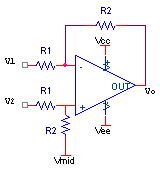
\includegraphics{schematics/differenceamp.PNG}
\end{center}
In this configuration each of the two inputs is connected to one of the op amp's inputs through a resistor ($R_1$).
Two additional resistors are used:
a feedback resistor from the output to the inverting input of the op amp, and another resistor of equal value from the non-inverting input of the op amp to the common mode voltage (usually $V\sub{CC}/2$ for a single supply system and GND for a dual supply system).
Using the fact that an ideal op amp's inputs are at equal voltages and \ac{kcl} on both the inverting and non-inverting inputs, the transfer function is

\textcolor{red}{
\begin{equation}
\vout = \frac{R_2}{R_1}(v_2 - v_1)
\label{eq:differenceamp}
\end{equation}
}

\subsection{High common-mode range difference amplifier}
\begin{center}
	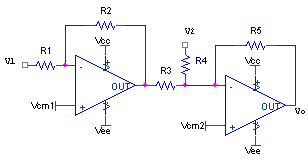
\includegraphics{schematics/highcmdifferenceamplifier.PNG}
\end{center}
This improved difference amplifier allows for a higher common-mode range because the resistors in series with the signal inputs $v_1$ and $v_2$ ($R_1$ and $R_4$, respectively) limit the currents into the op amps' inputs, increasing the voltage range within the op amp's drive capability. \autocite[418]{op-amps-for-everyone}

The transfer function can be derived easily using superposition and the above transfer functions for inverting and non-inverting op amp amplifiers to determine \vout in terms of all four inputs ($v_1$, $v_2$, $V\sub{CM1}$, and $V\sub{CM2}$).
For $v_1$,

\begin{equation}
\vout = \frac{R_2}{R_1}\frac{R_5}{R_3}v_1, v_2 = V\sub{CM1} = V\sub{CM2} = 0
\end{equation}

(the output of the first op amp is $-(R_2/R_1)v_1$, which is then amplified by $-R_5/R_3$).
For $v_2$,

\begin{equation}
\vout = -\frac{R_5}{R_4}v_2, v_1 = V\sub{CM1} = V\sub{CM2} = 0
\end{equation}

For $V\sub{CM1}$,

\begin{equation}
\vout = -\left(1+\frac{R_2}{R_1}\right)\frac{R_5}{R_3}V\sub{CM1}, v_{1} = v_{2} = V\sub{CM2} = 0
\end{equation}

For $V\sub{CM2}$,

\begin{equation}
\vout = \left(1+\frac{R_5}{R_3 \parallel R_4}\right)V\sub{CM2} = \left(1+\frac{(R_3+R_4)R_5}{R_3R_4}\right)V\sub{CM2}, v_1 = v_2 = V\sub{CM2} = 0
\end{equation}

Putting it all together,

\textcolor{red}{
\begin{equation}
\vout = \frac{R_2}{R_1}\frac{R_5}{R_3}v_1 - \frac{R_5}{R_4}v_2 - \left(1+\frac{R_2}{R_1}\right)\frac{R_5}{R_3}V\sub{CM1} + \left(1+\frac{(R_3+R_4)R_5}{R_3R_4}\right)V\sub{CM2}
\label{eq:highcmdifferenceamplifier}
\end{equation}
}

If all the resistors are equal, the transfer function simplifies to

\textcolor{red}{
\begin{equation}
\vout = v_1-v_2-2V\sub{CM1}+3V\sub{CM2}
\label{eq:highcmdifferenceamplifier_simple}
\end{equation}
}

% TODO
%\section{Op Amp Current Doubler}
% see p. 17 of the OPA454 datasheet. Slave amplifier is essentially a buffer in parallel with an op amp circuit (in any configuration)
% Also add somewhere that you can add a class B push-pull output stage to increase the current output of the op amp (see also p. 17 of the OPA454 datasheet). Put in a separate composite amplifier chapter?

\chapter{Instrumentation Amplifiers}

Instrumentation amplifiers are differential amplifiers just like operational amplifiers -- in fact, instrumentation amplifiers are constructed out of several operational amplifiers.
Instrumentation amplifiers, or in amps, have an extremely high input impedance.
This high input impedance is often achieved with a three op amp topology, using two of the op amps as input buffers or non-inverting amplifiers.
The in amp's input impedance is much higher than the op amp difference amplifier previously discussed, so the in amp is able to measure a differential voltage with much better accuracy.
In amps are often used to calibrate electronic instruments (hence the name \emph{instrumentation} amplifier) or to directly measure the small voltage signals from sensors (such as pressure transducers), voltage references, test equipment, etc.

While in amps can be constructed out of discrete op amps and resistors, the input op amps and all the resistors must be highly matched in order to minimize undesirable characteristics such as input offset voltage, common mode gain, etc.
As a result, in amps are usually constructed in integrated circuit form.

\section{Three op amp topology instrumentation amplifier}
\begin{center}
	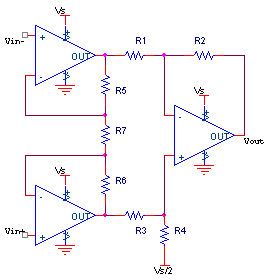
\includegraphics{schematics/threeinamp.PNG}
\end{center}
This is the standard, symmetric topology using three op amps.
To maintain symmetry (which, in this case, ensures each input voltage is amplified by the same amount), we must have

\begin{equation}
R_{5} = R_{6}
\end{equation}

\begin{equation}
R_{1} = R_{3}
\end{equation}

\begin{equation}
R_{2} = R_{4}
\end{equation}

The input differential voltage is

\begin{equation}
v_{diff} = v_{in+}-v_{in-}
\end{equation}

and it is the voltage across $R_{7}$ since the voltages at the inverting inputs of the input op amps are equal to the input voltages. The current through $R_{7}$ is thus

\begin{equation}
i_{R7} = \frac{v_{diff}}{R_{7}}
\end{equation}

The differential voltage between the two input op amps' outputs (call it $v_{o1}$) is

\begin{equation}
v_{o1} = i_{R7}(R_{5}+R_{6}+R_{7}) = i_{R7}(2R_{5}+R_{7}) = v_{diff}(1+2\frac{R_{5}}{R_{7}})
\end{equation}

The output op amp is configured as a difference amplifier with $v_{o1}$ as the input so the overall gain $A_{v}$ is

\textcolor{red}{
\begin{equation}
A_{v} = \frac{R_{2}}{R_{1}}(1+2\frac{R_{5}}{R_{7}})
\label{eq:threeinamp}
\end{equation}
}

$R_{5}$ and $R_{6}$ can be shorted and $R_{7}$ removed (replaced with an open circuit) to reduce the number of resistors -- this configures the input op amps as buffers.
The disadvantage, of course, is that the output op amp must be configured with a higher gain in order to achieve the same overall gain, which will reduce the in amp's bandwidth.

\section{Two op amp topology instrumentation amplifier}
\begin{center}
	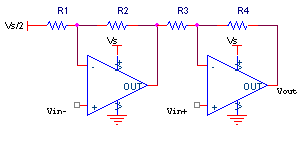
\includegraphics{schematics/twoinamp.PNG}
\end{center}
This in amp topology is less common but uses only two op amps, which can be useful to minimize the number of op amps used in the application circuit or to minimize power consumption.
As with the three op amp topology, resistors must be matched:

\begin{equation}
R_{1} = R_{4}
\end{equation}

\begin{equation}
R_{2} = R_{3}
\end{equation}

The transfer function is

\textcolor{red}{
\begin{equation}
A_{v} = 1+\frac{R_{1}}{R_{2}}
\label{eq:twoinamp}
\end{equation}
}

Unfortunately, this topology requires the $v_{in-}$ op amp to be used with less than unity gain (so it may be unstable) and the $v_{in-}$ signal has a higher propagation delay than the $v_{in+}$ signal.
Depending on the application circuit and the op amps available, the three op amp topology may have to be used instead.
\chapter{Filters}
This chapter presents a variety of filters (low pass, high pass, band pass, and band reject) using either passive or active components.
First and second order filters are presented so that an $n$th-order filter can be constructed by cascading these first and/or second order filters.

Some of these filters can be designed either as Butterworth or Chebyshev filters.
Butterworth filters are characterized by their maximally flat magnitude in the pass band for all-pole filters (so that, for all-pole filters, they are the best approximation to an ideal filter in the pass band).
Unfortunately, the magnitude of a Butterworth filter poorly approximates an ideal filter near the cutoff frequency in that the magnitude does not drop particularly sharply from the pass band to the stop band.
Higher order Butterworth filters transition more sharply and thus better approximate an ideal filter, but they are still inferior to filters like the Chebyshev filter.
Chebyshev filters' magnitude response best approximates an ideal filter for all-pole filters in that the magnitude drops very sharply from the pass band to the stop band, but their frequency response has ripples in the pass band (i.e. the magnitude oscillates in the pass band, particularly near the cutoff frequency).
Higher order Chebyshev filters transition even more sharply than lower order Chebyshev filters.
Thus, Butterworth and Chebyshev filters solve different problems -- the former approximates an ideal filter best in the pass band while the latter is a better approximation near the cutoff frequency. \autocite[107, 111]{op-amp-circuits-johnson}
% figure out where to put the tables for the coefficients

\section{Low pass filters}

\subsection{RC low pass passive filter}
\begin{center}
	\begin{circuitikz}
		\draw (0,0) node[above]{\vin} to[R=$R$, o-*] ++(2,0) coordinate(join)
		to[C=$C$] ++(0,-2) node[ground]{}
		(join) to[short, *-o] ++(1,0) node[above]{\vout};
	\end{circuitikz}
\end{center}
This is a very simple filter which can be easily analyzed using impedance.
Viewing the resistor and capacitor as an impedance divider:
\[\vout = \frac{\frac{1}{sC}}{R+\frac{1}{sC}}\vin\]
Rearranging, this is

\textcolor{red}{
\begin{equation}
\frac{v_{o}}{v_{i}}(s) = \frac{1}{sRC+1}
\label{eq:rcLPfilter}
\end{equation}
}

For low frequencies ($s \to 0$) $\vout/\vin \approx 1$ (all the voltage falls across the capacitor) and for high frequencies ($s \to \infty$) $\vout/\vin \approx 0$ (the capacitor has very low impedance so \vout is shorted to \gnd).

\subsection{First-order low pass active filter}
\begin{center}
	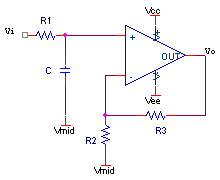
\includegraphics{schematics/1storderLPfilter.PNG}
\end{center}
The analysis of this circuit follows a similar approach as the op amp amplifier circuits.
The voltage at the inverting input (and thus the non-inverting input) is \[v_- = \frac{R_2}{R_2 + R_3}\vout\] (assuming for simplicity that $V\sub{MID} = \SI{0}{V}$) since $R_2$ and $R_3$ form a voltage divider.
\ac{kcl} on the non-inverting input node then relates this voltage with the input.
The transfer function is thus

\textcolor{red}{
\begin{equation}
\frac{\vout}{\vin}(s) = \frac{R_2 + R_3}{R_2(sR_1 C + 1)}
\label{eq:1storderLPfilter}
\end{equation}
}

This is clearly a low pass filter since $\vout/\vin \approx 1 + R_3/R_2$ for low frequencies where $sR_1 C \ll 1$ (notice the circuit behaves like an op amp non-inverting amplifier here) and $\vout/\vin \approx 0$ for high frequencies where $sR_{1}C \gg 1$.
In the limiting cases where $R_2 \to \infty$ and $R_3 \to 0$ the op amp is configured like a voltage buffer with an RC low pass filter at its input -- $R_2$ and $R_3$ simply provide gain in addition to the filtering operation.
If $R_2$ and $R_3$ are used, the three resistors should be chosen such that the filter formed by $R_1$ and $C$ has the desired \SI{-3}{dB} frequency and $R_1 = R_2 \parallel R_3$ (the latter relationship minimizes the error due to the op amp's input bias currents).

In this circuit $R_1$ and $C$ perform the same filtering function as the passive RC filter so the op amp isn't strictly necessary -- however, the op amp provides gain for the filter and can provide isolation of the RC filter from other circuit elements which might affect the its performance.

\subsection{Second-order \ac{vcvs} low pass active filter}
\begin{center}
	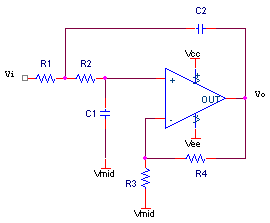
\includegraphics{schematics/2ndorder_vcvs_LPfilter.PNG}
\end{center}
This second order \ac{vcvs} low pass filter is similar in topology to the the above first order low pass filter except that it includes an extra resistor and capacitor. The full derivation of the input/output relationship requires a somewhat lengthy manipulation of equations, but it requires only three facts: (1) the voltage at the input terminals, which is $\frac{R_{3}}{R_{3}+R_{4}}v_{o}$ (again assuming that $v_{MID} = 0V$), (2) the nodal equation at the non-inverting input, and (3) the nodal equation at the node common to $R_{1}$, $R_{2}$, and $C_{2}$. This circuit is a second order filter so the transfer function is of the form

\textcolor{red}{
\begin{equation}
\frac{v_{o}}{v_{i}}(s) = \frac{Kb\omega_{c}^{2}}{s^{2} + a\omega_{c}s + b\omega_{c}^{2}}
\label{eq:2ndorder_vcvs_LPfilter}
\end{equation}
}

In this case

\begin{equation}
b\omega_{c}^{2} = \frac{1}{R_{1}R_{2}C_{1}C_{2}}
\end{equation}
\begin{equation}
a\omega_{c} = \frac{1}{C_{2}}\left(\frac{1}{R_{1}} + \frac{1}{R_{2}}\right) - \frac{R_{4}}{R_{2}R_{3}C_{1}}
\end{equation}
\begin{equation}
K = 1 + \frac{R_{4}}{R_{3}}
\end{equation}

To minimize the error due to the op amp's input bias currents we need

\begin{equation}
R_3 \parallel R_4 = R_1 + R_2
\end{equation}

With these restrictions and a desired gain $K$ and \SI{-3}{\dB} angular frequency $\omega_{c}$ we have the following equations for deciding the resistor and capacitor values \autocite[118-119]{op-amp-circuits-johnson}:

\begin{equation}
C_1 \leq \frac{(a^2+4b(K-1))C_2}{4b}
\end{equation}
\begin{equation}
R_1 = \frac{2}{(aC_2+\sqrt{(a^2+4b(K-1))C_2^2 - 4b C_1 C_2})\omega_{c}}
\end{equation}
\begin{equation}
R_2 = \frac{1}{bC_1 C_2 R_1\omega_{c}^2}
\end{equation}
\begin{equation}
R_3 = \frac{K(R_1 + R_2)}{K-1}, K > 1
\end{equation}
\begin{equation}
R_4 = K(R_1 + R_2)
\end{equation}

The parameters $a$ and $b$ depend on the type of filter desired -- Butterworth or Chebyshev. See Appendix A for tables of these parameter values.
% add appendix for the Butterworth and Chebyshev a and b coefficient parameters

\subsection{Second-order biquad low pass filter}
\begin{center}
	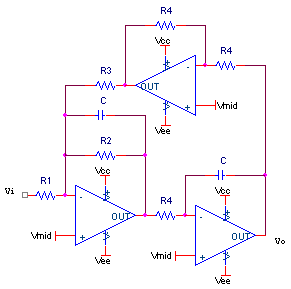
\includegraphics{schematics/2ndorderbiquadLPfilter.PNG}
\end{center}
The biquad filter requires two more op amps than the above \ac{vcvs} filters.
Two of the op amps are used as integrators and the third is an inverter.
The two integrators (which, of course, are low pass filters) form a second order low pass filter.
The transfer function can be determined by nodal analysis and noting the functions of each of the three op amps, but the full analysis is skipped.
Instead, the resistors and capacitors are simply given in terms of the general second-order low pass filter transfer function

\textcolor{red}{
\begin{equation}
\frac{v_{o}}{v_{i}}(s) = \frac{Kb\omega_{c}^{2}}{s^{2} + a\omega_{c}s + b\omega_{c}^{2}}
\label{eq:2ndorderbiquadLPfilter}
\end{equation}
}

The resistors relate to the general transfer function as follows:
\begin{equation}
R_4 = \frac{1}{\omega_{c}C}
\end{equation}
\begin{equation}
R_1 = \frac{R_4}{Kb}
\end{equation}
\begin{equation}
R_2 = \frac{R_4}{a}
\end{equation}
\begin{equation}
R_3 = \frac{R_4}{b}
\end{equation}

Why use the biquad circuit with its three op amps when a second order filter can be built with only one op amp?
Notice that the above equations for the biquad circuit's resistor and capacitor choices that the biquad is easier to tune than the \ac{vcvs} filters.
In particular, the desired $\omega_{c}$ determines the values of $C$ and $R_4$, and with $R_4$ chosen parameter $a$ is determined solely by $R_2$, parameter $b$ can be determined by $R_3$, and with $R_3$ determined $R_1$ can be used to set the filter's gain $K$.
The \ac{vcvs} filters require two different capacitor values and the resistors affect one or more values of $a$, $b$, and $K$ in nontrivial ways.
The biquad circuit's offer of simpler tuning may be worth the two additional op amps. \autocite[120-122]{op-amp-circuits-johnson}

\section{High pass filters}

\subsection{RC high pass passive filter}
\begin{center}
	\begin{circuitikz}
		\draw (0,0) node[above]{\vin} to[C=$C$, o-*] ++(2,0) coordinate(join)
		to[R=$R$] ++(0,-2) node[ground]{}
		(join) to[short, *-o] ++(1,0) node[above]{\vout};
	\end{circuitikz}
\end{center}
Compared to the low pass filter, the resistor and capacitor have been switched so the impedance divider is
\[\vout = \frac{R}{R+\frac{1}{sC}}\vin\]
Rearranged, this is

\textcolor{red}{
\begin{equation}
\frac{\vout}{\vin}(s) = \frac{sRC}{sRC+1}
\label{eq:rcHPfilter}
\end{equation}
}

\subsection{First-order high pass active filter}
\begin{center}
	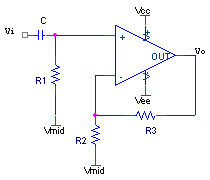
\includegraphics{schematics/1storderHPfilter.PNG}
\end{center}
Following the same approach as with the low pass active filter (using the resistor divider formed by $R_2$ and $R_3$ to calculate the op amp's input voltage in terms of \vout and using \ac{kcl} on the non-inverting input), the transfer function of the high pass filter is

\textcolor{red}{
\begin{equation}\frac{\vout}{\vin}(s) = \frac{sR_1 C \left(1 + \frac{R_3}{R_2}\right)}{sR_1 C + 1}
\label{eq:1storderHPfilter}
\end{equation}
}

For low frequencies ($s \to 0$) $\vout/\vin \approx 0$ and for high frequencies ($s \to \infty$) $\vout/\vin \approx 1 + R_3/R_2$ so the circuit behaves as a high pass filter.
As usual, the resistors should be chosen such that $R_1 = R_2 \parallel R_3$ to minimize the error due to the op amp's input bias currents.
If gain is not needed, the op amp can be configured as a voltage buffer by removing $R_2$ and replacing $R_3$ with a short.

\subsection{Second-order \ac{vcvs} high pass filter}
\begin{center}
	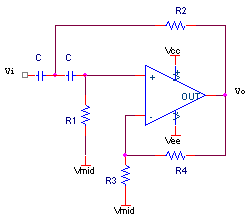
\includegraphics{schematics/2ndorder_vcvs_HPfilter.PNG}
\end{center}
The \ac{vcvs} second-order high pass filter is the same as the \ac{vcvs} second-order low pass filter but with the resistors replaced with capacitors and the capacitors replaced by resistors (except for the resister divider). Using the  general transfer function for a second-order high pass filter

\textcolor{red}{
\begin{equation}
\frac{v_{o}}{v_{i}}(s) = \frac{Ks^{2}}{s^{2} + \frac{a}{b}\omega_{c}s + \frac{\omega_{c}^{2}}{b}}
\label{eq:2ndorder_vcvs_HPfilter}
\end{equation}
}

the resistors determine the transfer function as follows \autocite[130-131]{op-amp-circuits-johnson}:
\begin{equation}
R_1 = \frac{4b}{(a+\sqrt{a^2 + 8b(K-1)})\omega_{c}C}
\end{equation}
\begin{equation}
R_2 = \frac{b}{\omega_{c}^2 C^2 R_1}
\end{equation}
\begin{equation}
R_3 = \frac{KR_1}{K-1}, K > 1
\end{equation}
\begin{equation}
R_4 = KR_1
\end{equation}

If no gain is needed (i.e. $K = 1$) $R_3$ can be removed and $R_4$ replaced with a short.

\subsection{Second-order biquad high pass filter}
\begin{center}
	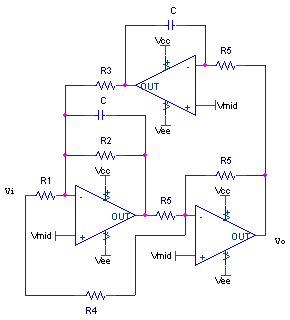
\includegraphics{schematics/2ndorderbiquadHPfilter.PNG}
\end{center}
This circuit is a biquad filter that implements the general second-order high pass filter transfer function

\textcolor{red}{
\begin{equation}
\frac{v_{o}}{v_{i}}(s) = \frac{Ks^{2}}{s^{2} + \frac{a}{b}\omega_{c}s + \frac{\omega_{c}^{2}}{b}}
\label{eq:2ndorderbiquadHPfilter}
\end{equation}
}

with an inverting gain (i.e. $K < 0$). The resistors relate to the transfer function as follows \autocite[131]{op-amp-circuits-johnson}:
\begin{equation}
R_1 = \frac{b}{aK\omega_{c}C}
\end{equation}
\begin{equation}
R_2 = KR_1
\end{equation}
\begin{equation}
R_3 = \frac{b}{\omega_{c}C}
\end{equation}
\begin{equation}
R_4 = \frac{1}{K\omega_{c}C}
\end{equation}
\begin{equation}
R_5 = \frac{1}{\omega_{c}C}
\end{equation}

\section{Band pass filters}

\subsection{\ac{vcvs} band pass filter}
\begin{center}
	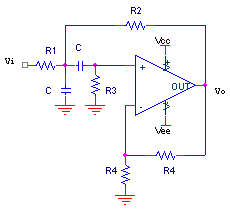
\includegraphics{schematics/vcvs_bandpass.PNG}
\end{center}
The general equation for the transfer function of this filter is

\textcolor{red}{
\begin{equation}
\frac{v_{o}}{v_{i}}(s) = \frac{\alpha \omega_{o}s}{s^{2}+\beta \omega_{o}s + \gamma \omega_{o}^{2}}
\label{eq:vcvs_bandpass}
\end{equation}
}

Since this is a band pass filter $\frac{v_{o}}{v_{i}} \approx 0$ as $s \rightarrow 0$ and $s \rightarrow \infty$ but the gain is nonzero in the midband. The resistors are related to the transfer function as follows \autocite[138-139]{op-amp-circuits-johnson}:
\begin{equation}
R_1 = \frac{2}{\alpha \omega_{o}C}
\end{equation}
\begin{equation}
R_2 = \frac{2}{(-\beta+\sqrt{(\alpha - \beta)^2 + 8\gamma})\omega_{o}C}
\end{equation}
\begin{equation}
R_3 = \frac{1}{\gamma \omega_{o}^2 C^2}\left(\frac{1}{R_1} + \frac{1}{R_2}\right)
\end{equation}
\begin{equation}
R_4 = 2R_3
\end{equation}

\subsection{Biquad band pass filter}
\begin{center}
	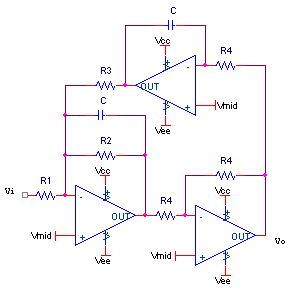
\includegraphics{schematics/biquad_bandpass.PNG}
\end{center}
The biquad band pass filter has the same transfer function as the \ac{vcvs} band pass filter:

\textcolor{red}{
\begin{equation}
\frac{v_{o}}{v_{i}}(s) = \frac{\alpha \omega_{o}s}{s^{2}+\beta \omega_{o}s + \gamma \omega_{o}^{2}}
\label{eq:biquad_bandpass}
\end{equation}
}

with the four resistors related to the transfer function as
\begin{equation}
R_1 = \frac{1}{\alpha \omega_{o}C}
\end{equation}
\begin{equation}
R_2 = \frac{1}{\beta \omega_{o}C}
\end{equation}
\begin{equation}
R_3 = \frac{1}{\gamma \omega_{o}C}
\end{equation}
\begin{equation}
R_4 = \frac{1}{\omega_{o}C}
\end{equation}

Again, the \ac{vcvs} band pass filter is simpler than the biquad but the latter is easier to tune than the former. \autocite[140]{op-amp-circuits-johnson}

\section{Band reject filters}

\subsection{Passive Twin-T band reject filter}
\begin{center}
	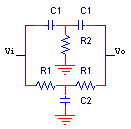
\includegraphics{schematics/passiveTwinTbandrejectfilter.PNG}
\end{center}
The intuitive way to understand that this circuit is a band reject filter is to realize that these are two T circuits in parallel -- one T circuit is composed of the two $R_1$ resistors and $C_2$ capacitor, and the other T circuit is composed of the two $C_1$ capacitors and $R_2$ resistor.
Consider each T individually:
the T circuit with the two resistors is a low pass filter since $C_2$ shorts the middle node to ground for high frequency signals and passes low frequency signals, and the T circuit with the two capacitors blocks low frequency signals but shorts \vin to \vout for high frequency signals.
Low frequencies can pass through the low pass T circuit and high frequencies can pass through the high pass T circuit, but there is a middle frequency that can pass through neither.
Thus, this Twin-T circuit is a band reject filter.

There are several methods for deriving the notch frequency, but the derivation is lengthy and not presented here.
The result of the derivation \autocite[see][]{cr-bond-twin-t-notch} is

\begin{equation}
	R_1C_1 = 4R_2C_2
\end{equation}

and

\begin{equation}
\omega^{2} = \frac{1}{2R_1R_2C_2^{2}}
\end{equation}

Usually the components are chosen such that $R_{2} = R_1/2$ and $C_2 = 2C_1$.
In that case, the notch frequency is

\textcolor{red}{
\begin{equation}
f = \frac{\omega}{2\pi} = \frac{1}{2\pi R_1C_1}
\label{eq:passiveTwinTnotchfreq}
\end{equation}
}

The limitation of this circuit is its quality factor $Q = 1/\Delta\Omega$, where $\Delta\Omega$ is the difference between the \SI{-3}{\dB} frequencies just above and below the notch frequency $f$.
For the passive Twin-T band reject filter,

\textcolor{red}{
\begin{equation}
Q = \frac{1}{4}
\label{passiveTwinT_Q}
\end{equation}
}

An active Twin-T band reject filter (which uses the Twin-T topology in the feedback path of an operational amplifier) improves $Q$. \autocite[321]{op-amps-for-everyone}

\subsection{Passive Wien-Robinson band reject filter}
\begin{center}
	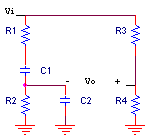
\includegraphics{schematics/passiveWien-Robinsonbandrejectfilter.PNG}
\end{center}
The Wien-Robinson band reject filter takes a single-ended input and produces a differential output.
It can be analyzed intuitively by realizing that it is composed of a voltage divider ($R_3$ and $R_4$) in parallel with a band pass filter.
$R_1$, $R_2$, $C_1$, and $C_2$ form a band pass filter because $C_1$ blocks low frequencies (no current passes through $C_1$ to create a voltage across $R_2$ and $C_2$) and $C_2$ shorts the band pass filter's output (the negative terminal of \vout) to ground, but midrange frequencies are passed to the output.
The overall circuit acts as a band reject filter because at low and high frequencies the negative terminal of \vout is grounded so that \[\vout = \frac{R_{3}}{R_{2}+R_{3}}v_{i}\]
At middle frequencies \vin is passed to the negative terminal of \vout so that the terminals of \vout are equal and $\vout = 0$.

This circuit suffers from a low $Q$ \autocite[323]{op-amps-for-everyone}, just as the passive Twin-T band reject filter (the two have similar values of $Q$).
It too can be improved with the use of operational amplifiers.

Typically the component values are chosen such that $R_1 = R_2$ and $C_1 = C_2$.
In that case the notch frequency \autocite[324]{op-amps-for-everyone} is

\textcolor{red}{
\begin{equation}
f = \frac{1}{2\pi R_{1}C_{1}}
\label{eq:passiveWienRobinson}
\end{equation}
}

\subsection{Active Twin-T band reject filter}
\begin{center}
	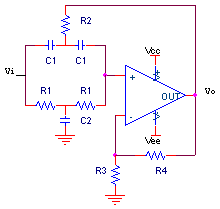
\includegraphics{schematics/activeTwinTbandrejectfilter.PNG}
\end{center}
The active Twin-T band reject filter adds an operational amplifer to the passive Twin-T filter.
The operational amplifier provides an increased gain and $Q$ since it is an active element.
$R_4$ provides negative feedback and $R_3$ sets the gain in the pass band (the filter circuitry has a gain of appoximately 1 in the pass band, so the circuit is essentially a non-inverting op amp amplifier).
The pass band gain $K$ is thus simply

\textcolor{red}{
\begin{equation}
K = 1 + \frac{R_{4}}{R_{3}}
\end{equation}
}

The filter circuitry itself is configured the same as that of the passive Twin-T filter, with the passive version's output node connected to the operational amplifier's non-inverting input and $R_2$ connected to the active filter's output.
Since the filter circuitry is the same, so is the notch frequency $f$.
Assuming the typical case of $R_2 = R_1/2$ and $C_2 = 2C_1$,

\textcolor{red}{
\begin{equation}
f = \frac{1}{2\pi R_{1}C_{1}}
\end{equation}
}

It can be shown \autocite[322]{op-amps-for-everyone} that the active Twin-T filter's $Q$ is

\textcolor{red}{
\begin{equation}
Q = \frac{1}{2(2-k)} = \frac{R_{3}}{2(R_{3}-R_{4})}
\end{equation}
}

With $K$ and $Q$ given in terms of the circuit components, the overall transfer function can be written in terms of the circuit components as well:

\textcolor{red}{
\begin{equation}
\frac{v_{o}}{v_{i}}(s) = \frac{K(s^{2}+1)}{s^{2}+\frac{s}{Q}+1} =  \frac{\frac{R_{3}+R_{4}}{R_{3}}(s^{2}+1)}{s^{2}+\frac{2(R_{3}-R_{4})}{R_{3}}s+1}
\end{equation}
}

\subsection{Active Wien-Robinson band reject filter}
\begin{center}
	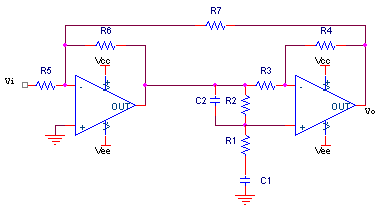
\includegraphics{schematics/activeWien-Robinsonbandrejectfilter.PNG}
\end{center}
The active Wien-Robinson band reject filter uses two operational amplifiers to improve the passive Wien-Robinson filter's $Q$ and gain.
The resistors and capacitors which compose the passive Wien-Robinson filter are labeled the same in the above schematic of the active version as in the passive version from before.
The inputs of the operational amplifier which drives the overall output are driven by the filter's differential output.
The other operational amplifier is configured simply as an inverting amplifier.
The transfer function \autocite[323]{op-amps-for-everyone} can be written as

\textcolor{red}{
\begin{equation}
\frac{v_{o}}{v_{i}}(s) = \frac{\frac{R_{6}R_{7}}{R_{5}(R_{6}+R_{7})}(s^{2}+1)}{s^{2}+\frac{3R_{7}}{R_{6}+R_{7}}s+1}
\label{eq:activeWienRobinsonbandreject}
\end{equation}
}

If $R_1 = R_2$ and $C_1 = C_2$ as is typical, then

\textcolor{red}{
\begin{equation}
f = \frac{1}{2\pi R_1 C_1}
\end{equation}
}

since the filtering circuitry is unchanged from the passive version.
$Q$ can be determined by inspection since it is the coefficient of the first order $s$ term,

\textcolor{red}{
\begin{equation}
Q = \frac{3R_7}{R_6 + R_7}
\end{equation}
}

and the active filter's passband gain $K$ can also be determined by inspection:

\textcolor{red}{
\begin{equation}
K = \frac{R_6 R_7}{R_5(R_6 + R_7)}
\end{equation}
}

The active Wien-Robinson band reject filter differs from its active Twin-T counterpart in that the passband gain $k$ can be chosen without affecting the quality factor $Q$.

\subsection{\ac{vcvs} band reject filter}
\begin{center}
	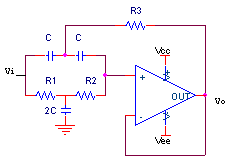
\includegraphics{schematics/vcvs_bandreject.PNG}
\end{center}
This band reject filter's transfer function can be written in the form

\textcolor{red}{
\begin{equation}
\frac{\vout}{\vin}(s) = \frac{s^2 + \omega_{o}^2}{s^2 + \frac{\omega_{o}}{Q}s + \omega_{o}^2}
\label{eq:vcvs_bandreject}
\end{equation}
}

The op amp is configured as a voltage follower and, since it is the only active device in the circuit, the overall gain of this filter can never exceed unity even in the pass band.
To achieve the desired transfer function the resistors must be chosen as follows \autocite[145-146]{op-amp-circuits-johnson}:
\begin{equation}
R_1 = \frac{1}{2Q\omega_{o}C}
\end{equation}
\begin{equation}
R_2 = \frac{2Q}{\omega_{o}C}
\end{equation}
\begin{equation}
R_3 = \frac{R_1 R_2}{R_1 + R_2}
\end{equation}

\subsection{Biquad band reject filter}
\begin{center}
	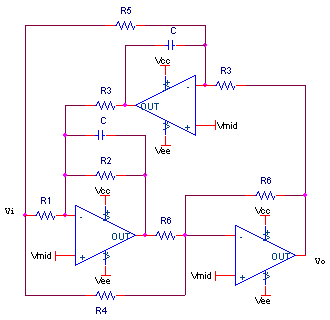
\includegraphics{schematics/biquad_bandreject.PNG}
\end{center}
A band reject filter's transfer function can also be written in the form 

\textcolor{red}{
\begin{equation}
\frac{v_{o}}{v_{i}}(s) = \frac{\alpha (s^{2} + \omega_{o}^{2})}{s^{2} + \beta \omega_{o}s + \gamma \omega_{o}^{2}}
\label{eq:biquad_bandreject}
\end{equation}
}

Unlike the \ac{vcvs} band reject filter above, this biquad filter can provide an inverting gain greater than unity (the $\alpha$ term), and it can also achieve a much higher $Q$.
The resistors relate to the transfer function as \autocite[146-148]{op-amp-circuits-johnson}
\begin{equation}
R_1 = \frac{1}{\alpha \beta \omega_{o}C}
\end{equation}
\begin{equation}
R_2 = \alpha R_1
\end{equation}
\begin{equation}
R_3 = \frac{1}{\sqrt{\gamma} \omega_{o}C}
\end{equation}
\begin{equation}
R_4 = \frac{1}{\alpha \omega_{o}C}
\end{equation}
\begin{equation}
R_5 = \frac{\sqrt{\gamma}}{\alpha \omega_{o}C}
\end{equation}
\begin{equation}
R_6 = \frac{1}{\omega_{o}C}
\end{equation}

\section{All pass filters}
\subsection{First-order all pass filter}
\begin{center}
	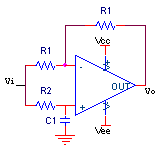
\includegraphics{schematics/1storderallpassfilter.PNG}
\end{center}
This circuit \autocite[328]{op-amps-for-everyone} has a gain of 1 at low frequencies and -1 at high frequencies.
At low frequencies, neither the capacitor nor the non-inverting input of the operational amplifier draw any current, so there is no voltage drop across $R_2$ and the non-inverting input has a voltage equal to \vin.
The inverting input also has a voltage equal to \vin since the operational amplifier's inputs must be at (approximately) equal voltage, so there is no voltage drop across the $R_1$ connected to \vin.
Since there is no voltage drop across (or current through) the $R_1$ connected to \vin, there is no current through (or voltage drop across) the $R_1$ connected to \vout. Thus, $\vout = \vin$ at low frequencies.
At high frequencies, the non-inverting input of the operational amplifier is shorted to ground since the capacitor has a very low impedance.
$R_2$ does nothing to the circuit since it is only connected to \vin and \gnd and the circuit looks like an inverting op amp amplifier, which of course has a gain of -1 when the gain and feedback resistors ($R_1$, in this case) are equal.

It is not intuitively obvious, however, that the circuit has a gain of magnitude 1 in the middle of the frequency spectrum, so we need to derive the transfer function.
Let the voltage at the operational amplifier's inputs be $v_x$.
$R_2$ and $C_1$ act as a voltage divider for \vin at the operational amplifier's inverting input, so

\begin{equation}v_x = \frac{\frac{1}{sC_1}}{R_2 + \frac{1}{sC_1}}\vin = \frac{\vin}{1+sR_2 C_1}
\end{equation}

The operational amplifier's non-inverting input is also at voltage $v_x$ (ideally), so use \ac{kcl} at the non-inverting input node:

\begin{equation}
\frac{\vout-v_x}{R_1} = \frac{v_x - \vin}{R_1}
\end{equation}

Substituting for $v_{x}$, we have

\begin{equation}
\frac{\vout}{R_1}-\frac{\vin}{R_1(1+sR_2 C_1)} = \frac{\vin}{R_1(1+sR_2 C_1)}-\frac{\vin}{R_1}
\end{equation}

Rearranging, we have

\begin{equation}
\vout = \vin\left(\frac{2}{1+sR_2 C_1}-1\right)
\end{equation}

Rearranging further, the transfer function is thus

\textcolor{red}{
\begin{equation}
\frac{\vout}{\vin}(s) = \frac{1-sR_2 C_1}{1+sR_2 C_1}
\label{eq:1storderallpassfilter}
\end{equation}
}

The transfer function reveals a zero at $s = 1/(R_2 C_1)$ and a pole at $s = -1/(R_2 C_1)$ (technically, the operational amplifier introduces its own poles to the system so that the gain does actually go to zero at very high frequencies, but we are assuming that the frequencies of operation are well below the operational amplifier's poles).
In any case, the gain has constant magnitude $|H(s)| = |H(\jmath\omega)|$ across the (operational) frequency spectrum since

\begin{equation}
|H(\jmath\omega)| = \frac{\sqrt{1+(-\omega R_2 C_1)^2}}{\sqrt{1+(\omega R_2 C_1)^2}} = 1
\end{equation}

so the circuit is an all pass filter.
The point of an all pass filter is that it can change a system's phase response across the frequency spectrum -- the phase changes from $0$ to $-\pi$ radians from low to high frequency.
More specifically, the phase $\angle H(s) = \angle H(\jmath\omega)$ is

\textcolor{red}{
\begin{equation}
\angle H(\jmath\omega) = \tan^{-1}(-\omega R_2 C_1) - \tan^{-1}(\omega R_2 C_1) = -2\tan^{-1}(\omega R_2 C_1)
\label{eq:1storderallpassfilter_angle}
\end{equation}
}

Although the values of $R_2$ and $C_1$ do not affect the magnitude of the circuit's gain across the frequency spectrum, they must be chosen appropriately to shape the circuit's phase response over frequency as desired.
$R_1$ can be any reasonable value, of course, since the $R_1$ resistors do not directly affect the transfer function.

\subsection{Second-order all pass filter}
\begin{center}
	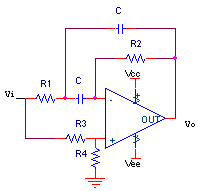
\includegraphics{schematics/2ndorder_allpass.PNG}
\end{center}
A second order all pass filter has the transfer function

\textcolor{red}{
\begin{equation}
\frac{\vout}{\vin}(s) = H(s) = \frac{K(s^2 - a\omega_{o}s + b\omega_{o}^2)}{s^2 + a\omega_{o}s + b\omega_{o}^2}
\label{eq:2ndorder_allpass}
\end{equation}
}

since this transfer function has two poles and

\begin{equation}
|H(\jmath\omega)| = K\frac{\sqrt{(b\omega_{o}^2-\omega^2) + (-a\omega_{o}\omega)^2}}{\sqrt{(b\omega_{o}^2-\omega^2) + (a\omega_{o}\omega)^2}} = K
\end{equation}

The phase is

\textcolor{red}{
\begin{equation}
\angle H(\jmath\omega) = \tan^{-1}\left(-\frac{b\omega_{o}^2-\omega^2}{a\omega_{o}\omega}\right) - \tan^{-1}\left(\frac{b\omega_{o}^2-\omega^2}{a\omega_{o}\omega}\right) = -2\tan^{-1}\left(\frac{b\omega_{o}^2-\omega^2}{a\omega_{o}\omega}\right)
\label{eq:2ndorder_allpass_angle}
\end{equation}
}

This circuit implements the second order all pass filter transfer function, with the resistors chosen such that
\begin{equation}
a\omega_{o} = \frac{2}{R_2 C}
\end{equation}
\begin{equation}
b\omega_{o}^2 = \frac{1}{R_1 R_2 C^2}
\end{equation}
\begin{equation}
K = \frac{R_4}{R_3 + R_4}
\end{equation}
\begin{equation}
4R_1 R_4 = R_2 R_3
\end{equation}

For minimum DC offset, choose \autocite[151-153]{op-amp-circuits-johnson}:

\begin{equation}
R_2 = \frac{R_3 R_4}{R_3 + R_4}
\end{equation}
\chapter{Compensators}
Compensators modify the loop transfer function $L(s)$ of a feedback system to stabilize the system or improve its performance.
Compensators add one or more poles and/or zeros to $L(s)$ to change the feedback system's steady-state error, noise rejection, crossover frequency $\omega_{c}$, phase margin $\phi_{M}$, gain margin, etc.
There are three types of compensators: lag, lead, and lead-lag compensators.

Lag compensators have a low frequency pole and a higher frequency zero so they have a transfer function of the form \[G_{c}(s) = K\frac{\tau_{1}s+1}{\tau_{2}s+1}, \tau_{1} < \tau_{2}\]
Lag compensators are typically used either to decrease $|L(s)|$ at high frequencies while maintaining a high $|L(s)|$ at low frequencies, or to increase $|L(s)|$ at low frequencies without also increasing $|L(s)|$ at high frequencies.
The latter is more common, and decreases the system's steady state error and improves its disturbance rejection but maintains $\omega_{c}$, $\phi_{M}$, and (high frequency) noise rejection. \autocite[269]{analog-design-feedback-lundberg}

Lead compensators have a low frequency zero and high frequency pole so a lead compensator's transfer function is of the form \[G_{c}(s) = K\frac{\alpha \tau_{1}s+1}{\tau_{2}s+1}, \tau_{1} > \tau_{2}\]
The phase increases (i.e. moves away from $-\pi$) between the zero and pole's frequency, so $\phi_{M}$ can be increased if the zero and pole are placed such that $\omega_{c}$ is greater than the zero's frequency but less than the pole's frequency.
The maximum increase in phase between the compensator's zero and pole is given by $\phi = \arcsin \frac{\alpha - 1}{\alpha + 1}$.
A typical value of $\alpha = 10$ yields $\phi = 55\,^{\circ}$.
$\alpha$ should not be too high, however, because the higher the value of $\alpha$ the greater the increase in high frequency gain (which reduces high frequency noise rejection).
The easiest way to design a lead compensator is to place the zero at $\omega_{c}$ -- if $\alpha$ is high enough (i.e. the pole is at a high enough frequency) the phase margin $\phi_{M}$ can be increased by approximately $45\,^{\circ}$ and $\omega_{c}$ is not changed significantly.
To maximize the increase in $\phi_{M}$, however, the zero and pole should be placed such that their geometric mean is equal to $\omega_{c}$. \autocite[277-278]{analog-design-feedback-lundberg}

The benefits of both a lead and lag compensator can be acheived with a lead-lag compensator, which can be as simple as cascading a lag compensator and lead compensator.
The lag compensator can improve the low frequency characteristics of the plant while the lead compensator improves the plant's transfer function near $\omega_{c}$.

\section{Passive lag compensator}
\begin{center}
	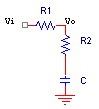
\includegraphics{schematics/passivelag.PNG}
\end{center}
This lag compensator is constructed out of passive components. It cannot achieve a gain greater than 1 (i.e. $K > 1$), of course, but in cases where such a gain is not necessary this compensator can reduce the feedback system's power consumption versus an active lag compensator. It is easy to see how this is a lag compensator: at low frequencies the capacitor is an open circuit so the impedance to ground is much higher than $R_{1}$ and $\frac{v_{o}}{v_{i}}(s) = 1$, and at high frequencies the capacitor is a short so $R_{1}$ and $R_{2}$ form a simple voltage divider which gives $\frac{v_{o}}{v_{i}}(s) = \frac{R_{2}}{R_{1}+R_{2}}$. To be more precise, this is a voltage divider consisting of impedances $R_{1}$ and $R_{2}+\frac{1}{sC}$. The transfer function \autocite[270]{analog-design-feedback-lundberg} is therefore

\textcolor{red}{
\begin{equation}
\frac{\vout}{\vin}(s) = \frac{R_2+\frac{1}{sC}}{R_1 + R_2 + \frac{1}{sC}} = \frac{sR_2 C + 1}{1+s(R_1 + R_2)C}
\label{eq:passivelagcompensator}
\end{equation}
}

An alternative passive lag compensator places the capacitor in parallel with $R_2$ rather than in series with it:
\begin{figure}[h]
	\centering
		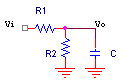
\includegraphics{schematics/passivelag2.PNG}
	\caption{Alternative passive lag compensator}
	\label{fig:passivelag2}
\end{figure}

This too is a voltage divider, but this time the impedances are $R_1$ and $R_2 \parallel C$.
The transfer function is $\frac{\vout}{\vin}(s) = \frac{R_2 \parallel C}{R_1 + R_2 \parallel C} = \frac{R_2}{R_1 + R_2 +sR_1 R_2 C}$, which is best expressed as

\textcolor{red}{
\begin{equation}
\frac{\vout}{\vin}(s) = \frac{R_2}{R_1 + R_2}\frac{1}{1+s(R_1 \parallel R_2)C}
\end{equation}
}

to make the DC gain and the location of the pole obvious.

\section{Passive lead compensator}
\begin{center}
	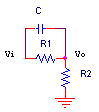
\includegraphics{schematics/passivelead.PNG}
\end{center}
This lead compensator is very similar to the above passive lag compensator. In this case, at low frequencies the capacitor is an open circuit so $R_{1}$ and $R_{2}$ simply form a voltage divider to give $\frac{v_{o}}{v_{i}}(s) = \frac{R_{2}}{R_{1}+R_{2}}$, and at high frequencies the capacitor shorts $R_{1}$ so that $\frac{v_{o}}{v_{i}}(s) = 1$. The full analysis isn't much more difficult: this is an voltage divider consisting of impedances $R_{1}||\frac{1}{sC} = \frac{R_{1}}{1+sR_{1}C}$ and $R_{2}$. The transfer function is thus

\textcolor{red}{
\begin{equation}
\frac{v_{o}}{v_{i}}(s) = \frac{R_{2}}{\frac{R_{1}}{sR_{1}C+1} + R_{2}} = \frac{R_{2}(sR_{1}C + 1)}{(R_{1} + R_{2})(s\frac{R_{1}R_{2}}{R_{1}+R_{2}}C + 1)}
\label{eq:passivelead}
\end{equation}
}

The latter expression puts the transfer function in the $K\frac{\alpha \tau_1 s+1}{\tau_2 s+1}$ form to make the gain and time constants clear. \autocite[278]{analog-design-feedback-lundberg}

\section{Passive lead-lag compensator}
\begin{center}
	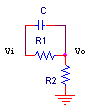
\includegraphics{schematics/passiveleadlag.PNG}
\end{center}
This lead-lag compensator provides the benefits of both a lead compensator and a lag compensator and does it entirely with passive components. Its transfer function is fairly easy to derive since this circuit is a voltage divider using the impedances $R_1 \parallel \frac{1}{sC}$ and $R_2$.
Since

\begin{equation}
R_1 \parallel C = \frac{R_1}{1+sR_1 C}
\end{equation}
we have
\begin{equation}
\frac{\vout}{\vin}(s) = \frac{R_2}{R_2 + \frac{R_1}{1+sR_1 C}} = \frac{R_2(1+sR_1 C)}{R_1 + R_2 + sR_1 R_2 C}
\end{equation}

By factoring out $R_1 + R_2$ we get

\textcolor{red}{
\begin{equation}
\frac{\vout}{\vin}(s) = \frac{R_2}{R_1 + R_2}\frac{1+sR_1 C}{1+s(R_1 \parallel R_2)C}
\label{eq:passiveleadlag}
\end{equation}
}

The location of the zero is determined first by choosing appropriate values of $R_1$ and $C$, and $R_2$ determines the location of the pole.

\section{Active lag compensator}
\begin{center}
	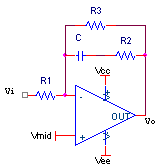
\includegraphics{schematics/activelag.PNG}
\end{center}
This is a basic lag compensator constructed with an operational amplifier so that a choice of $K > 1$ is possible. It is the same as an inverting amplifier except that a capacitor and resistor in series are placed in parallel with the feedback resistor. The same analysis can be used as the one for the inverting amplifer except that the feedback impedance is $R_{3}||(R_{2}+\frac{1}{sC})$. The transfer function is

\textcolor{red}{
\begin{equation}
\frac{v_{o}}{v_{i}}(s) = -\frac{R_{3}}{R_{1}}\frac{1+sR_{2}C}{1+s(R_{2} + R_{3})C}
\label{eq:activelag}
\end{equation}
}

This compensator can also be used as a proportional-plus-integral (sometimes abbreviated P+I or PI) compensator by removing $R_3$ \autocite[270]{analog-design-feedback-lundberg}:

\textcolor{red}{
\begin{equation}
\frac{\vout}{\vin}(s) = - \frac{1+sR_2 C}{sR_1 C}
\label{eq:P+I}
\end{equation}
}

\section{Active lead compensator}
\begin{center}
	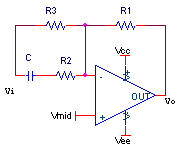
\includegraphics{schematics/activelead.PNG}
\end{center}
This is a fairly simple lead compensator which uses an operational amplifier to provide $K > 1$. It is the same as an inverting amplifier except that a capacitor and resistor in series are placed in parallel with the input resistor. The same analysis can be used as the one for the inverting amplifer except that the impedance from \vin to the op amp's inverting input is $R_3 \parallel (R_2 + \frac{1}{Cs})$. The transfer function \autocite[278]{analog-design-feedback-lundberg} is thus

\textcolor{red}{
\begin{equation}
\frac{\vout}{\vin}(s) = -\frac{R_1}{R_3}\frac{1+s(R_2 + R_3)C}{1+sR_2C}
\label{eq:activelead}
\end{equation}
}

\section{Type I active compensator}
\begin{center}
	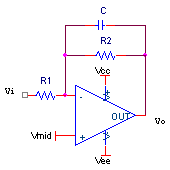
\includegraphics{schematics/type1compensator.PNG}
\end{center}
This compensator is essentially a low pass filter since it has a single pole and no zeroes. It can be used to lower the plant's gain at higher frequencies exactly as a low pass filter and thus improve high frequency noise rejection, or it can be used a dominant pole compensator if the DC gain $\frac{R_{2}}{R_{1}}$ is chosen sufficiently high and the compensator's pole is chosen to be a sufficiently low frequency. The transfer function is the same as that of an op amp in an inverting amplifier configuration, except that the feedback impedance is
\begin{equation}
R_{2}||C = \frac{R_{2}}{1+sR_{2}C}
\end{equation}

Thus it is

\textcolor{red}{
\begin{equation}
\frac{v_{o}}{v_{i}}(s) = -\frac{R_{2}}{R_{1}}\frac{1}{1+sR_{2}C}
\label{eq:type1compensator}
\end{equation}
}

\section{Type II active compensator}
\begin{center}
	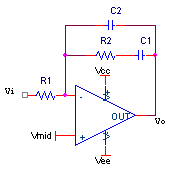
\includegraphics{schematics/type2compensator.PNG}
\end{center}
This compensator is a bit more complex: it has a zero, a pole at the origin, and a second pole. The pole at the origin is caused by the two capacitors in the feedback path; since both are open circuits at DC there is no feedback path at DC and the DC gain is the op amp's open loop gain. To derive the transfer function use the fact that the op amp is configured as an inverting amplifier but with a feedback impedance of
\begin{equation}
\left(R_{2}+\frac{1}{sC_{1}}\right)||\frac{1}{sC_{2}} = \frac{1+sR_{2}C_{1}}{s(sR_{2}C_{1}C_{2}+C_{1}+C_{2})}
\end{equation}

Dividing this impedance by $-\frac{1}{R_{1}}$ and rearranging, we see the transfer function is

\textcolor{red}{
\begin{equation}
\frac{v_{o}}{v_{i}}(s) = -\frac{1+sR_{2}C_{1}}{sR_{1}(C_{1}+C_{2})(1+sR_{2}\frac{C_{1}C_{2}}{C_{1}+C_{2}})}
\label{eq:type2compensator}
\end{equation}
}

\section{Type III active compensator}
\begin{center}
	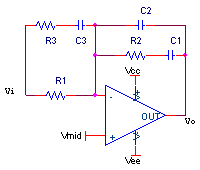
\includegraphics{schematics/type3compensator.PNG}
\end{center}
This compensator is even more complex because it adds a resistor and capacitor to the input network and in doing so adds another zero and pole for a total of two zeroes, a pole at the origin, and two additional poles. So many zeroes and poles make this a very flexible compensator that can significantly improve a plant's transfer function, but at the cost of complexity. Fortunately, we have already done most of the work in deriving the transfer function since this compensator's feedback network is the same as that of the type II compensator above. The input network is now
\begin{equation}
R_{1}||\left(R_{3}+\frac{1}{sC_{3}}\right) = \frac{R_{1}(1+sR_{3}C_{3})}{1+s(R_{1}+R_{3})C_{3}}
\end{equation}

and so the transfer function is

\textcolor{red}{
\begin{equation}
\frac{v_{o}}{v_{i}}(s) = -\frac{(1+sR_{2}C_{1})(1+s(R_{1}+R_{3})C_{3})}{sR_{1}(C_{1}+C_{2})(1+sR_{3}C_{3})(1+sR_{2}\frac{C_{1}C_{2}}{C_{1}+C_{2}})}
\label{eq:type3compensator}
\end{equation}
}
%\chapter{Diode Circuits}

Diodes are nonlinear circuit elements so many diode circuits are nonlinear in nature. Diodes can be used in circuits to rectify AC voltages, clamp and clip voltages, etc. Special diodes, such as Zener diodes, can be used for still other applications such as generating a voltage reference or biasing a bipolar transistor.

\section{Half-wave rectifier (Neamen p.63)}
% Add capacitor in parallel with the load resistor for a DC voltage
\section{Full-wave rectifier (Neamen p.67)}

\section{Full-wave bridge rectifier (Neamen p.68)}
%For the three above circuits a negative voltage can be generated by reversing %the direction of the diodes.
\section{Voltage doubler (Neamen p. 79)}

\section{Zener diode voltage regulator (Neamen p. 80)}
%Remember to note that v_out is usually followed with an op amp buffer.

\section{Voltage clipper (Neamen p. 88)}
%The voltage sources in the circuit on p.88 can be replaced with Zeners as in %the circuit on p. 90.
\section{Voltage clamper (Neamen p. 91)}

\section{Diode OR logic gate (Neamen p. 100)}

\section{Diode AND logic gate (Neamen p. 101)}
%\chapter{Advanced Operational Amplifier Circuits}

\section{T network feedback loop (Op Amps for Everyone, p. 422)}

\section{Simulated inductor}

\section{Automatic Gain Control (AGC) amplifier}

\section{Logarithmic amplifier (Diode) (p.227)}

\section{Logarithmic amplifier (BJT) (p.228)}

\section{One-shot multivibrator (p.234)}

\section{Ohmmeter (p.243)}

\section{Capacitance meter (p.243)}

\section{Capacitance multiplier}
% from https://electronics.stackexchange.com/q/602959

\section{Transistor test circuit (p.245)}

\section{Zener diode tester (p.245)}

\section{Precision half-wave rectifier (p.246)}

\section{Peak detector (p.247)}
\chapter{Transistor-Level Amplifiers and Buffers}
This chapter presents some very basic amplifiers and buffers built out of transistors.
These circuits are very common in transistor level circuit designs, and many are used as components of operational amplifiers.
Without these basic circuits none of the circuits in the previous chapters would be possible since they are the basis of operational amplifiers.

The two most common types of transistors are \acp{bjt} and \acp{mosfet}.
There are two different types of bipolar transistors -- \textit{npn} and \textit{pnp}.
Similarly, MOSFETs are either NMOS or PMOS.
BJTs and MOSFETs can be constructed in various ways to exhibit different characteristics -- some bipolar transistors have larger emitter areas or are designed to have a higher $\beta_{F}$, for example, and some MOSFETs are designed to handle high power or to have a low $R\sub{DS(on)}$.
The transistors in the circuits that follow, however, are all general purpose; the only variation is between \textit{npn} and \textit{pnp} for bipolar transistors and NMOS and PMOS for MOSFETs.

Many of the circuits that follow can be implemented with either bipolar transistors or MOSFETs.
The analysis of both implementations are usually very similar so in some cases only the bipolar version is shown and analyzed.
The impedance into the gate of a MOSFET can be approximated as infinite but the same is not true for the base of a bipolar transistor, so the bipolar implementation is occasionally more complicated;
analysis of only the bipolar implementation is thus slightly more general and informative than analysis of only the MOS implementation.

Although the analysis of bipolar implementations cannot approximate the impedance into the base as infinite, one can approximate impedances into the base and emitter of a bipolar transistor using the principle of \textit{$\beta_{F}$ impedance reflection}.
\textit{Impedance reflection} allows one to approximate the impedance into the base of a bipolar transistor as the impedance at the base (e.g. $r_{\pi}$) plus the impedance at the emitter multiplied by $\beta_{F} + 1$ (or $\beta_{0} + 1$, for small signals).
Thus, a resistor $R_{E}$ connected from the emitter to signal ground results in a total impedance looking into the base of $r_{\pi} + (\beta_{F} + 1)R_{E}$.
Similarly, the impedance looking into the emitter is the impedance at the emitter plus the impedance at the base divided by $\beta_{F} + 1$.

For most of these circuits the transistor's base (or gate) must be biased to a certain \DC voltage depending on the desired $I_{C}$ (or $I_{D}$). Biasing a MOSFET with a resistor divider is trivial since the bias voltage $V_{G}$ generated by the resistor divider is not affected by a current into or out of the MOSFET's gate (there is ideally no such current since there is an ideally infinite impedance into the gate).
A bipolar transistor, on the other hand, has a small but non-negligible base current $I_{B}$ which can have an effect on $V_{B}$ if the bias resistors are chosen incorrectly.
To ensure the resistor divider generates the desired $V_{B}$, a good rule of thumb is to choose resistors such that the current through the bias resistors is at least ten times $I_{B}$ -- this ensures the current through the bias resistors is not so small that $I_{B}$ affects $V_{B}$ while not dissipating too much power.
Some of the circuits that follow show resistor dividers, which are assumed to be chosen to meet these constraints.
There are, of course, other methods to properly bias the transistor(s).

There are several other rules of thumb regarding transistors.
One is that a change in voltage applied to the gate/base of a transistor will, in general, result in the source/emitter swinging in the same direction as the gate/base and the drain/collector swinging in the opposite direction;
this can be used to determine whether a signal is inverted or not through a path of transistors.
Another rule of thumb is that impedances looking into a source/emitter are low and impedances looking into a drain/collector and gate/base are high, and dominant time constants are typically located in nodes with high impedances.

\section*{Bipolar equations}
\begin{equation}
I_{C} = I_{S}\left(e^{\frac{V_{BE}}{V_{TH}}}-1\right)
\label{eq:bipolarIc}
\end{equation}

\begin{equation}
I_{C} = \beta_{F}I_{B}
\label{eq:bipolarIcwrtIb}
\end{equation}

\begin{equation}
I_{E} = I_{B} + I_{C} = \frac{\beta_{F}+1}{\beta_{F}}I_{C}
\label{eq:bipolarIewrtIc}
\end{equation}

\section*{MOS equations}

In the active region with strong inversion:
\begin{equation}
I_{D} = \frac{\mu_{n}C_{ox}}{2}\frac{W}{L}\left(V_{GS}-V_{t}\right)^{2}\left(1+\frac{V_{DS}}{V_{A}}\right), V_{GS} \geq V_{t}, V_{GD} < V_{t}
\label{eq:activeId}
\end{equation}

\begin{equation}
\chi = \frac{g_{mb}}{g_{m}}
\label{eq:chi}
\end{equation}

In the active region with weak inversion:
\begin{equation}
I_{D} = \frac{W}{L}I_{t}e^{\frac{V_{GS}-V_{t}}{nV_{t}}}\left(1-e^{-\frac{V_{DS}}{V_{t}}}\right)
\label{eq:Idweakinversion}
\end{equation}

\noindent where

\begin{equation}
I_{t} = qXD_{n}n_{po}e^{\frac{k_{2}}{V_{T}}}
\end{equation}

\noindent and

\begin{equation}
\frac{1}{n} = \frac{1}{1+\chi}
\label{eq:Id_n}
\end{equation}

\section*{Small Signal Models}
The complete hybrid-$\pi$ small-signal model \autocite[33]{analysis-design-analog-ics} for both \textit{npn} and \textit{pnp} bipolar transistors is shown in Figure \ref{fig:complete_bipolar_hybrid_pi}. The complete MOS small-signal model \autocite[55]{analysis-design-analog-ics} is shown in Figure \ref{fig:complete_MOS_ss_model} and is also valid for both NMOS and PMOS transistors.

\begin{figure}[h]
	\centering
		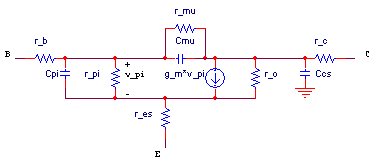
\includegraphics{schematics/complete_bipolar_hybrid_pi.PNG}
	\caption{Complete bipolar hybrid-pi model}
	\label{fig:complete_bipolar_hybrid_pi}
\end{figure}
\begin{figure}[h]
	\centering
		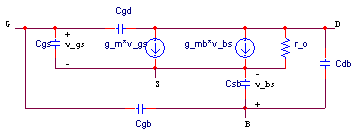
\includegraphics{schematics/complete_MOS_ss_model.PNG}
	\caption{Complete MOS small-signal model}
	\label{fig:complete_MOS_ss_model}
\end{figure}

It is usually not necessary to use the complete hybrid-$\pi$ or MOS small signal model, and attempting to use the complete models usually makes the small-signal analysis overly complicated.
For hand calculations with the hybrid-$\pi$ small-signal model one can usually treat $C_{\pi}$, $r_{\mu}$, $C_{\mu}$, and $C_{cs}$ as open circuits, and $r_{es}$ and $r_{c}$ as a short circuit.
For hand calculations with the MOS small-signal model one can usually treat all the capacitors as open circuits.
Additionally, one can usually ignore the $g_{mb}v_{bs}$ dependent current source since the MOSFET's backgate is usually connected to the source.
Unless specifically stated otherwise, the following analyses assume the backgate is connected to the source so $g_{mb}v_{bs} = 0$.

\section{Common emitter/source}
\begin{center}
	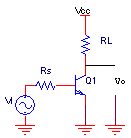
\includegraphics{schematics/basiccommonemitter.PNG}
\end{center}
\par
The common emitter (or common source) is so named because in this configuration the emitter/source of the transistor is shorted to a common signal source (in this case, $GND$). The output is taken from the transistor's collector (or drain). Sometimes the common emitter/source is used with a resistor connected from the emitter/source to the common signal source; such a resistor is called an \textit{emitter degeneration} resistor or \textit{source degeneration} resistor. Emitter/source degeneration employs negative feedback in the form of an impedance to provide temperature stability to the circuit at DC -- a common emitter without emitter degeneration has $v_{BE} = v_{B} = v_{I}$ (where $v_{B}$ is the voltage at the transistor's base) and $i_{C} = I_{S}e^{\frac{v_{I}}{V_{th}}}$ so $v_{O} = V_{CC} - R_{L}I_{S}e^{\frac{v_{I}}{V_{th}}}$. Lack of emitter degeneration therefore gives high gain (since the $v_{I}$ term is part of an exponential) at the expense of temperature stability (since the temperature-dependent $V_{th}$ term is also in the exponential). Such a tradeoff is a familiar concept in control theory. For an AC signal, however, emitter/source degeneration can be used to provide DC stability without sacrificing gain by using an appropriately sized emitter/source capacitor $C_{E}$ (or $C_{S}$) in parallel with the emitter/source degeneration resistor $R_{E}$ (or $R_{S}$) that has (ideally) zero impedance at all frequencies of the input signal. The DC stability provided by the emitter degeneration resistor ensures that the transistor is biased correctly so that it behaves linearly for the small signal input while the emitter/source capacitor maintains high gain for input AC signals.
\par
If the common emitter/source is used for processing AC signals but not DC, it is usually necessary to use a DC blocking capacitor in series with the output of the preceding stage and the transistor's base. Figure \ref{fig:commonemitter} shows the common emitter with a DC blocking capacitor, a voltage divider to bias the transistor's base, an emitter degeneration resistor, and an emitter bypass capacitor.

\subsection{Bipolar}
\begin{figure}[h]
	\centering
		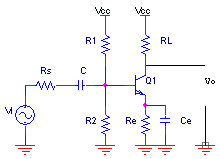
\includegraphics{schematics/commonemitter.PNG}
	\caption{Common emitter implementation for AC signals}
	\label{fig:commonemitter}
\end{figure}
\par
To analyze the small signal behavior of the common emitter one can use a slightly simplified version of the hybrid-$\pi$ small signal model. Also, assume the DC blocking capacitor is a short circuit for the frequencies of interest and, to derive as general a transfer function as possible, assume an emitter degeneration resistor is used without an emitter bypass capacitor. For simplicity assume that $R_{1}$ and $R_{2}$ are large enough that they can be ignored and define $R_{S}' = R_{S}+r_{b}$. Figure \ref{fig:ss_commonemitter} shows the small signal model of this common emitter circuit.
\begin{figure}[h]
	\centering
		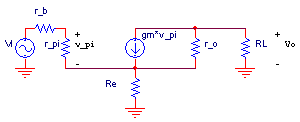
\includegraphics{schematics/ss_commonemitter.PNG}
	\caption{Common emitter small signal model}
	\label{fig:ss_commonemitter}
\end{figure}
\par
It is easy enough to derive the transfer function of the common emitter without emitter degeneration since with $R_{E} = 0$ the emitter is shorted to ground and the input section ($v_{i}$, $r_{b}$, and $r_{\pi}$) is isolated from the output section ($g_{m}v_{\pi}$, $r_{o}$, and $R_{L}$). However, for the general case (i.e. with emitter degeneration) it is easier to view the common emitter as an equivalent two port small-signal model as shown in Figure \ref{fig:twoport_ss_model} and derive the input resistance $R_{i}$, output resistance $R_{o}$, and transconductance $G_{m}$ (note that $G_{m}$ is not to be confused with the transistor's transconductance $g_{m}$ -- it is $G_{m} = \frac{i_{o}}{v_{i}}$ with the output shorted).
\begin{figure}
	\centering
		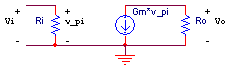
\includegraphics{schematics/twoport_ss_model.PNG}
	\caption{Two port equivalent small-signal model}
	\label{fig:twoport_ss_model}
\end{figure}
\par
To derive $R_{i}$, $R_{o}$, and $G_{m}$ start with Ohm's Law and KCL at the emitter and collector. By Ohm's Law,

\begin{equation}
i_{b} = \frac{v_{i}-v_{e}}{r_{\pi}}
\label{eq:common_emitter_i_b}
\end{equation}

\noindent (where $v_{e}$ is the voltage at the emitter and $i_{b}$ is the small-signal base current and also the circuit's small-signal input current). KCL at the emitter yields

\begin{equation}
\frac{v_{e}}{R_{E}} + \frac{v_{e}+i_{o}R_{L}}{r_{o}} = (\beta_{0}+1)i_{b}
\label{eq:common_emitter_KCL_emitter}
\end{equation}

\noindent (recall that $g_{m}v_{\pi} = \beta_{0}i_{b}$). KCL at the collector yields

\begin{equation}
i_{o} + \frac{v_{e}+i_{o}R_{L}}{r_{o}} = i_{o}\left(1 + \frac{R_{L}}{r_{o}}\right) + \frac{v_{e}}{r_{o}} = \beta_{0}i_{b}
\label{eq:common_emitter_KCL_collector}
\end{equation}

\noindent Solving for $i_{o}$ in (\ref{eq:common_emitter_KCL_emitter}), substituting it into (\ref{eq:common_emitter_KCL_collector}), and rearranging, we find

\begin{equation}
v_{e} = i_{b}\left(\frac{1+(\beta_{0}+1)\frac{r_{o}}{R_{L}}}{\frac{1}{R_{L}} + \frac{1}{R_{E}} + \frac{r_{o}}{R_{L}R_{E}}}\right)
\label{eq:common_emitter_v_e}
\end{equation}

Substituting (\ref{eq:common_emitter_v_e}) into (\ref{eq:common_emitter_i_b}) (which can be rewritten as $R_{i} = \vin/i_b = \rpi + v_e/i_b$), we find \autocite[197-199]{analysis-design-analog-ics}

\textcolor{red}{
\begin{equation}
R_{i} = r_{\pi} + (\beta_{0}+1)\left(\frac{r_{o} + \frac{R_{L}}{\beta_{0}+1}}{r_{o} + R_{L} + R_{E}}\right)R_{E}
\label{eq:common_emitter_Ri}
\end{equation}
}

\par
Often $r_{o} >> R_{L}$ and $r_{o} >> R_{E}$ so (\ref{eq:common_emitter_Ri}) can be approximated as

\textcolor{red}{
\begin{equation}
R_{i} \approx r_{\pi} + (\beta_{0}+1)R_{E}
\label{eq:common_emitter_Ri_approx}
\end{equation}
}

Note that this approximation is consistent with the principle of \textit{$\beta_{F}$ impedance reflection}.

For the circuit's transconductance $G_{m}$ set $R_{L} = 0$ (since the output is shorted by definition of $G_{m}$). From the emitter KCL equation $\frac{v_{e}}{R_{E}} + \frac{v_{e}}{r_{o}} = (\beta_{0} + 1)i_{b} = (\beta_{0} + 1)\frac{v_{i}-v_{e}}{r_{\pi}}$ so

\begin{equation}
v_{e} = \frac{\frac{\beta_{0}+1}{r_{\pi}}}{\frac{1}{R_{E}} + \frac{1}{r_{o}} + \frac{1}{r_{\pi}}}v_{i}
\label{eq:common_emitter_v_e2}
\end{equation}

From the collector KCL equation we know

\begin{equation}
i_{o} + \frac{v_{e}}{r_{o}} = \beta_{0}i_{b} = \beta_{0}\frac{v_{i}-v_{e}}{r_{\pi}}
\label{eq:common_emitter_KCL_collector2}
\end{equation}

so we can substitute (\ref{eq:common_emitter_v_e2}), which is in terms of \vin, to find \autocite[199]{analysis-design-analog-ics}

\textcolor{red}{
\begin{equation}
G_{m} = g_{m}\frac{1-\frac{R_{E}}{\beta_{0}r_{o}}}{1 + g_{m}R_{E}\left(1 + \frac{1}{\beta_{0}} + \frac{1}{g_{m}r_{o}}\right)}
\label{eq:common_emitter_Gm}
\end{equation}
}

Often $r_{o} \gg R_{E}$, $\beta_{0} \gg 1$, and $g_{m}r_{o} \gg 1$ so

\textcolor{red}{
\begin{equation}
G_{m} \approx \frac{g_{m}}{1 + g_{m}R_{E}}
\label{eq:common_emitter_Gm_approx}
\end{equation}
}

Without emitter degeneration ($R_{E} = 0$) both equations reduce to $G_{m} = g_{m}$, which is expected since the common emitter's hybrid-$\pi$ small-signal model looks like the two port small-signal model when the emitter is shorted to ground.

It is clear from the two port model (Figure \ref{fig:twoport_ss_model}) that $\vout = -G_{m}r_{o}\vin$ so using (\ref{eq:common_emitter_Gm}) we know

\textcolor{red}{
\begin{equation}
\frac{\vout}{\vin} = g_{m}\frac{1-\frac{R_E}{\beta_0 r_o}}{1 + g_m R_E\left(1 + \frac{1}{\beta_0} + \frac{1}{g_m r_o}\right)}r_o
\label{eq:commonemitter_transferfunction}
\end{equation}
}

\begin{figure}
	\centering
		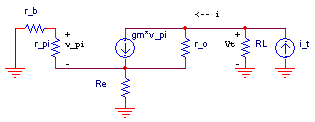
\includegraphics{schematics/commonemitter_Ro.PNG}
	\caption{Common emitter small-signal equivalent model for computing output resistance}
	\label{fig:commonemitter_Ro}
\end{figure}

To find the small-signal output resistance $R_{o}$ of the common emitter, use the equivalent circuit shown in Figure \ref{fig:commonemitter_Ro}. Using a test current source $i_{t}$ and the voltage $v_{t}$ across it, $R_{o}$ is, by definition,

\begin{equation}
R_{o} = \frac{v_{t}}{i_{t}}
\end{equation}

\noindent By defining $i$ as the portion of the $i_{t}$ current into the $g_{m}v_{\pi}$ current source and $r_{o}$, this becomes

\begin{equation}
R_{o} = \frac{v_{t}}{i}||R_{L}
\end{equation}

\noindent The current $i$ splits between the $g_{m}v_{\pi}$ current source and $r_{o}$ but recombines at the emitter node so

\begin{equation}
v_{\pi} = -i\frac{r_{\pi}R_{E}}{r_{\pi}+R_{E}}
\label{eq:commonemitter_Ro_v_pi}
\end{equation}

\noindent assuming $r_{b}$ is small enough to be ignored (if not, simply add it to $r_{\pi}$). Also, the current $i_{1}$ through $r_{o}$ is

\begin{equation}
i_{1} = i - g_{m}v_{\pi} = i + ig_{m}\frac{r_{\pi}R_{E}}{r_{\pi}+R_{E}}
\label{eq:commonemitter_Ro_i_1}
\end{equation}

\noindent where the latter equation is true by substituting $-i(r_{\pi}||R_{E})$ for $v_{\pi}$ using (\ref{eq:commonemitter_Ro_v_pi}). Using (\ref{eq:commonemitter_Ro_v_pi}) and (\ref{eq:commonemitter_Ro_i_1}), the voltage $v_{t}$ is thus

\begin{equation}
v_{t} = i_{1}r_{o}-v_{\pi} = i\frac{r_{\pi}R_{E}}{r_{\pi}+R_{E}} + ir_{o}\left(1+g_{m}\frac{r_{\pi}R_{E}}{r_{\pi}+R_{E}}\right)
\label{eq:commonemitter_Ro_v_t}
\end{equation}

\noindent Dividing both sides of (\ref{eq:commonemitter_Ro_v_t}) by $i$ and putting the result in parallel with $R_{L}$ gives \autocite[200]{analysis-design-analog-ics}

\textcolor{red}{
\begin{equation}
R_{o} = \left(\frac{r_{\pi}R_{E}}{r_{\pi}+R_{E}} + r_{o}\left(1+g_{m}\frac{r_{\pi}R_{E}}{r_{\pi}+R_{E}}\right)\right) \parallel R_{L}
\label{eq:commonemitter_Ro}
\end{equation}
}

The first term is much smaller than the second so
\textcolor{red}{
\begin{equation}
R_{o} \approx r_{o}\left(1+g_{m}\frac{r_{\pi}R_{E}}{r_{\pi}+R_{E}}\right) \parallel R_{L} = r_{o}\left(1+\frac{g_{m}R_{E}}{1+\frac{g_{m}R_{E}}{\beta_{0}}}\right) \parallel R_{L}
\end{equation}
}

Depending on whether $\beta_{0}$ is significantly larger or smaller than $g_{m}R_{E}$, $R_{o}$ can be further simplified as follows:

\textcolor{red}{
\begin{equation}
R_{o} \approx (r_{o}(1+g_{m}R_{E})) \parallel R_{L}\text{, }\beta_{0} \gg g_{m}R_{E}
\end{equation}
}

\textcolor{red}{
\begin{equation}
R_{o} \approx (r_{o}(1+\beta_{0})) \parallel R_{L}\text{, }g_{m}R_{E} \gg \beta_{0}
\end{equation}
}

\subsection{MOS}
The small signal model of the common source is identical to the common emitter hybrid-$\pi$ model shown in Figure \ref{fig:ss_commonemitter}, except that $r_{\pi} \rightarrow \infty$ and the $g_{m}v_{\pi}$ current source is replaced with two current sources ($g_{m}v_{gs}$ and $g_{mb}v_{bs}$) in parallel (assuming the body terminal is connected to GND or $V_{SS}$, whichever is the lowest supply voltage). First we find $G_{m} = \frac{i_{o}}{v_{i}}$ using KCL at the source and at the drain (with $R_{L} = 0$):

\begin{equation}
\frac{v_{s}}{R_{S}} + \frac{v_{s}}{r_{o}} = g_{m}v_{gs} + g_{mb}v_{bs} = g_{m}(v_{i}-v_{s}) - g_{mb}v_{s}
\label{eq:commonsource_KCL_source}
\end{equation}

\begin{equation}
i_{o} + \frac{v_{s}}{r_{o}} = g_{m}v_{gs} + g_{mb}v_{bs} = g_{m}(v_{i}-v_{s}) - g_{mb}v_{s}
\label{eq:commonsource_KCL_drain}
\end{equation}

Solving (\ref{eq:commonsource_KCL_source}) for $v_{s}$ yields

\begin{equation}
v_{s} = \frac{g_{m}v_{i}}{g_{m}+g_{mb}+\frac{1}{R_{S}}+\frac{1}{r_{o}}}
\label{eq:commonsource_v_s}
\end{equation}

Substituting (\ref{eq:commonsource_v_s}) into (\ref{eq:commonsource_KCL_drain}) and rearranging yields \autocite[201]{analysis-design-analog-ics}

\textcolor{red}{
\begin{equation}
G_{m} = \frac{g_{m}}{1+(g_{m}+g_{mb})R_{S}+\frac{R_{S}}{r_{o}}}
\end{equation}
}

In the case where $r_{o} \gg R_{S}$, the equation for $G_{m}$ simplifies to

\textcolor{red}{
\begin{equation}
G_{m} \approx \frac{g_m}{1+(g_m + g_{mb})R_S}
\end{equation}
}

The common source's output resistance $R_{o}$ can be computed the same way as the common emitter's $R_{o}$: we apply a test current $i_{t}$ into the output and measure the voltage $v_{t}$ across the current source (as before, temporarily ignore $R_{L}$ and add it back in parallel) to find $R_{o} = \frac{v_{t}}{i_{t}}$.
The test current $i_{t}$ is also the current through $R_{S}$ since none of it is diverted through a finite $r_{\pi}$ so

\begin{equation}
v_{s} = i_{t}R_{S}
\label{eq:commonsource_Ro_v_s}
\end{equation}

If $i_{1}$ is the current through $r_{o}$, \ac{kvl} shows that

\begin{equation}
v_{t} = i_{1}r_{o}+v_{s} = (i_{t}-g_{m}v_{gs}-g_{mb}v_{bs})r_{o}+v_{s} = (i_{t}+g_{m}v_{s}+g_{mb}v_{s})r_{o}+v_{s}
\label{eq:commonsource_Ro_v_t}
\end{equation}

\noindent Substituting (\ref{eq:commonsource_Ro_v_s}) into (\ref{eq:commonsource_Ro_v_t}), rearranging, and then putting the result in parallel with $R_{L}$ yields

\textcolor{red}{
\begin{equation}
R_{o} = (R_{S} + (1+(g_{m}+g_{mb})R_{S})r_{o}+R_{S}) \parallel R_{L}
\label{eq:commonsource_Ro}
\end{equation}
}

The common source's input resistance $R_{i}$ is trivially

\textcolor{red}{
\begin{equation}
R_{i} = \infty
\end{equation}
}

\section{Common collector/drain (emitter/source follower)}
\begin{center}
	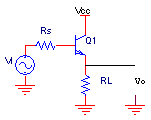
\includegraphics{schematics/basicemitterfollower.PNG}
\end{center}

In this circuit the collector or drain is shorted to the supply voltage so it is called a common collector (or common drain). It is also known as the emitter follower (or source follower) since \vout is the voltage across the emitter (or source) resistor and follows the base voltage (which is also the input voltage \vin). The circuit has a voltage gain of approximately unity so it is a voltage follower (buffer).

As will be seen in the full analysis, emitter/source followers have a high $R_{i}$. This makes them useful loads for voltage amplifiers (such as common emitters/sources) so that most of the preceding amplifier's output voltage falls across the emitter/source follower's input. The full analysis will also show that emitter/source followers have a low $R_{o}$, which makes them useful sources for circuits that require an input voltage since an ideal voltage source has zero $R_{o}$. Emitter/source followers are also used to push out poles that would otherwise appear in a circuit by reducing the resistance seen by a node where a capacitance appears (a high resistance seen by a capacitor can result in a long RC time constant, degrading the circuit's response at higher frequencies). Emitter/source followers are thus highly useful circuits even when processing voltage signals.

\subsection{Bipolar}
For the emitter follower it is easy to see from (\ref{eq:bipolarIc}) that the voltage gain is approximately unity even without a full analysis. Assuming a constant temperature so $V_{TH}$ does not vary, $v_{BE}$ does not vary significantly even for relatively large variations in $I_{C}$ due to the exponential relationship between $v_{BE}$ and $I_{C}$. Since $v_{BE}$ does not vary then $v_{E} = v_{O}$ must follow $v_{B} = v_{I}$.
\begin{figure}[h]
	\centering
		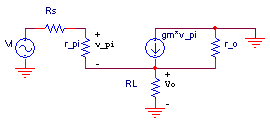
\includegraphics{schematics/ss_emitterfollower.PNG}
	\caption{Emitter follower small signal model}
	\label{fig:ss_emitterfollower}
\end{figure}

Although the preceding first order analysis proves that the voltage gain is approximately unity, it is often necessary to know the exact transfer function. To find it, use KCL at the emitter:

\begin{equation}
i_{i}+\beta_{0} i_{i} - \frac{v_{o}}{R_{L}} - \frac{v_{o}}{r_{o}} = 0
\label{eq:emitter_follower_KCL_output}
\end{equation}

\noindent where $i_{i}$ is the current into the base of the transistor. Since $i_{i}$ flows through $R_{S}$ (which may include the transistor's base resistance $r_{b}$, if such accuracy is needed) and $r_{\pi}$, and the voltage across these two resistors is $v_{be} = v_{i} - v_{o}$, 

\begin{equation}
i_{i} = \frac{v_{i}-v_{o}}{R_{S}+r_{\pi}}
\label{eq:emitter_follower_i_i}
\end{equation}

\noindent Substituting into (\ref{eq:emitter_follower_KCL_output}) and rearranging terms, the transfer function is

\textcolor{red}{
\begin{equation}
\frac{v_{o}}{v_{i}} = \frac{1}{1+\frac{R_{S}+r_{\pi}}{(\beta_{0} + 1)(R_{L}||r_{o})}}
\label{eq:emitter_follower}
\end{equation}
}

\noindent If $(\beta_{0} + 1)(R_{L}||r_{o}) >> R_{S}+r_{\pi}$ then the voltage gain is approximately unity. Another common approximation of the transfer function is

\textcolor{red}{
\begin{equation}
\frac{v_{o}}{v_{i}} \approx \frac{g_{m}R_{L}}{1+g_{m}R_{L}}
\label{eq:emitter_follower_approx}
\end{equation}
}

\noindent which is true when $\beta >> 1$, $r_{\pi} >> R_{S}$, and $r_{o} >> R_{L}$.
\par
The input resistance $R_{i}$ of the emitter follower can be determined by removing the input voltage source (including its resistance $R_{S}$) and measuring the equivalent resistance looking into the input terminals. Similarly, the output resistance $R_{o}$ can be determined by removing the load resistor $R_{L}$ and measuring the equivalent resistance looking into the output terminals. However, both $R_{i}$ and $R_{o}$ can be determined by inspection using \textit{impedance reflection}:

\textcolor{red}{
\begin{equation}
R_{i} = r_{\pi} + (\beta_{0} + 1)(R_{L}||r_{o})
\label{eq:emitter_follower_Ri}
\end{equation}
}

\textcolor{red}{
\begin{equation}
R_{o} = \frac{R_{S}+r_{\pi}}{\beta_{0} + 1}||r_{o}
\label{eq:emitter_follower_Ro}
\end{equation}
}

\noindent The latter simplifies to

\textcolor{red}{
\begin{equation}
R_{o} \approx \frac{1}{g_{m}} + \frac{R_{S}}{\beta_{0} + 1}
\label{eq:emitter_follower_Ro_approx}
\end{equation}
}

\noindent if $\beta >> 1$ and $r_{o} >> \frac{R_{S}+r_{\pi}}{\beta_{0} + 1}$.
\newpage
\begin{figure}[h]
	\centering
		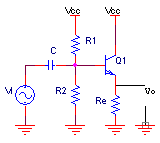
\includegraphics{schematics/emitterfollower.PNG}
	\caption{Emitter follower implementation for AC signals}
	\label{fig:emitterfollowerAC}
\end{figure}
\par
An emitter follower implementation for AC signals is shown above in Figure \ref{fig:emitterfollowerAC}. It includes bias resistors $R_{1}$ and $R_{2}$ which of course affect $R_{i}$ -- add $R_{1}||R_{2}$ in parallel with (\ref{eq:emitter_follower_Ri}).

\subsection{MOS}
The source follower also has a voltage gain of approximately unity, a fact which can be seen from the square-law dependence of $I_{D}$ on $V_{GS}$ in the active region as shown by (\ref{eq:activeId}) -- $V_{GS}$ does not vary significantly even for relatively large variations in $I_{D}$. $V_{GS}$ does vary with $I_{D}$ more than the bipolar transistor's $V_{BE}$ varies with its $I_{C}$, however, so a source follower's voltage gain is generally less than unity and more so than the emitter follower's voltage gain. The full small signal analysis will demonstrate this.
\begin{figure}[h]
	\centering
		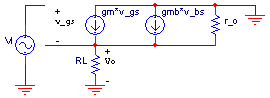
\includegraphics{schematics/ss_sourcefollower.PNG}
	\caption{Source follower small signal model}
	\label{fig:ss_sourcefollower}
\end{figure}
\par
With the MOSFET's body terminal connected to the lowest supply voltage (GND) in the small signal model shown in Figure \ref{fig:ss_sourcefollower}, we can determine the transfer function exactly by realizing that

\begin{equation}
v_{bs} = -v_{s} = -v_{o}
\end{equation}

\noindent and finding KCL at the output (the source):

\begin{equation}
g_{m}v_{gs} - g_{mb}v_{o} = \frac{v_{o}}{R_{L}} + \frac{v_{o}}{r_{o}}
\label{eq:sourcefollower_KCL}
\end{equation}

\noindent Also, KVL around the input loop shows that

\begin{equation}
v_{i} = v_{o} + v_{gs}
\label{eq:sourcefollower_KVL}
\end{equation}

\noindent Solving (\ref{eq:sourcefollower_KCL}) for $v_{gs}$ and substituting the result into (\ref{eq:sourcefollower_KVL}) gives

\textcolor{red}{
\begin{equation}
\frac{v_{o}}{v_{i}} = \frac{g_{m}}{g_{m} + g_{mb} + \frac{1}{R_{L}} + \frac{1}{r_{o}}} = \frac{g_{m}r_{o}}{(g_{m} + g_{mb})r_{o} + 1 + \frac{r_{o}}{R_{L}}}
\label{eq:sourcefollower}
\end{equation}
}

\noindent In the case where $R_{L} \rightarrow \infty$, (\ref{eq:sourcefollower}) simplifies to

\textcolor{red}{
\begin{equation}
\frac{v_{o}}{v_{i}} \approx \frac{g_{m}r_{o}}{1+(g_{m}+g_{mb})r_{o}}
\end{equation}
}

% TODO: figure out how to do lim -> \infty
\noindent If both $R_{L} \rightarrow \infty$ and $r_{o} \rightarrow \infty$ then

\begin{equation}
\frac{v_{o}}{v_{i}} \approx \frac{g_{m}}{g_{m}+g_{mb}} = \frac{1}{1+\chi}
\end{equation}

\noindent where $\chi$ is defined in (\ref{eq:chi}) and is typically well below unity (in the range of 0.2).
\par
The voltage gain can be improved by tying the MOSFET's body to its source so that $v_{bs} = 0$ and the $g_{mb}$ term disappears:

\textcolor{red}{
\begin{equation}
\frac{v_{o}}{v_{i}} = \frac{g_{m}r_{o}}{1+g_{m}r_{o} + \frac{r_{o}}{R_{L}}}
\label{eq:sourcefollower_no_gmb}
\end{equation}
}

\textcolor{red}{
\begin{equation}
\frac{v_{o}}{v_{i}} \approx \frac{g_{m}r_{o}}{1+g_{m}r_{o}}
\end{equation}
}

The input resistance $R_{i}$ of the source follower is the resistance looking into the gate of the MOSFET, which is trivially

\textcolor{red}{
\begin{equation}
R_{i} = \infty
\end{equation}
}

The output resistance $R_{o}$ is the resistance looking into the output with $v_{i} = 0$. Since $v_{i} = 0$ it is obvious that

\begin{equation}
v_{gs} = -v_{o}
\end{equation}

\noindent Also, KCL at the output yields

\begin{equation}
i_{o} = \frac{v_{o}}{r_{o}} + \frac{v_{o}}{R_{L}} + (g_{m}+g_{mb})v_{o}
\label{eq:sourcefollower_Ro_io}
\end{equation}

\noindent Rearranging (\ref{eq:sourcefollower_Ro_io}) gives an equation for $R_{o}$:

\textcolor{red}{
\begin{equation}
R_{o} = \frac{1}{g_{m}+g_{mb}+\frac{1}{r_{o}}+\frac{1}{R_{L}}}
\label{eq:sourcefollower_Ro}
\end{equation}
}

\section{Common base/gate}
\begin{center}
	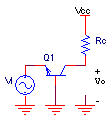
\includegraphics{schematics/commonbase.PNG}
\end{center}
The transistor in a common base/gate circuit is biased such that the base/gate is directly connected to AC ground, the input is applied to the emitter/source, and the output is taken from the collector/drain. Although the input and output signals are voltages, it is useful to think of the common base/gate as a current source (since $I_{C} \approx I_{E}$ and $I_{D} \approx I_{S}$) with a high $R_{o}$ (the resistance looking into the collector/drain is $r_{o}$, which is usually very high). These characteristics of the common base/gate make it useful in certain situation, such as a cascode circuit (see below).

\subsection{Bipolar}
\par
The transfer function and input and output resistances of the previous circuits were derived using the hybrid-$\pi$ small signal model, but the dependent $g_{m}v_{\pi}$ current source is directly connected from output to input and thus makes the analysis of the hybrid-$\pi$ small signal model for the common base difficult. One way to simplify the analysis of the common base circuit is to transform the hybrid-$\pi$ model into an equivalent \textsl{T model}. The first step in this tranformation is to split the $g_{m}v_{\pi}$ current source into two current sources of value $g_{m}v_{\pi}$, with one connected from the collector to the base and the other connected from the base to the emitter. Splitting the $g_{m}v_{\pi}$ current source like this is possible since the currents entering and exiting the base are equal (i.e. KCL at the base is unchanged) and the two current sources supply the same current from collector to emitter. Next, note that the $g_{m}v_{\pi}$ dependent current source from the collector to the base is controlled by the voltage across it -- so its equivalent resistance $r_{cb}$ is

\begin{equation}
r_{cb} = \frac{v_{\pi}}{g_{m}v_{\pi}} = \frac{1}{g_{m}}
\end{equation}

\noindent and we can replace the dependent current source with a resistor that is in parallel with $r_{\pi}$. The parallel combination of these two resistors is the equivalent resistance $r_{e}$, which is

\begin{equation}
r_{e} = \frac{\frac{r_{\pi}}{g_{m}}}{\frac{1}{g_{m}}+r_{\pi}} = \frac{1}{\frac{1}{r_{\pi}}+g_{m}} = \frac{1}{g_{m}\left(1+\frac{1}{\beta_{0}}\right)}
\end{equation}

At low frequencies the capacitors and resistors $r_{o}$ and $r_{\mu}$ can be neglected, in which case the small signal model looks like a ``T''. The transformation from the hybrid-$\pi$ model to the \textsl{T model} with and without the higher frequency elements is shown in Figures \ref{fig:ss_commonbase_hybrid_pi} - \ref{fig:ss_commonbase_T_model_approx}. \autocite[183-184]{analysis-design-analog-ics}

\begin{figure}[h]
	\centering
		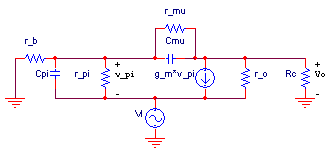
\includegraphics{schematics/ss_commonbase_hybrid_pi.PNG}
	\caption{Hybrid-$\pi$ small signal model for common base analysis}
	\label{fig:ss_commonbase_hybrid_pi}
\end{figure}

\begin{figure}[h]
	\centering
		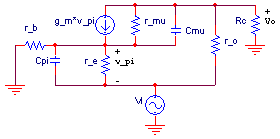
\includegraphics{schematics/ss_commonbase_T_model.PNG}
	\caption{Small signal \textsl{T model} for common base analysis}
	\label{fig:ss_commonbase_T_model}
\end{figure}

\begin{figure}[h]
	\centering
		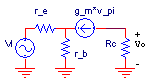
\includegraphics{schematics/ss_commonbase_T_model_approx.PNG}
	\caption{Small signal \textsl{T model} for common base at low frequencies}
	\label{fig:ss_commonbase_T_model_approx}
\end{figure}

With this simplified model it is trivial to see that

\textcolor{red}{
\begin{equation}
R_{o} = R_{C}
\label{eq:common_base_Ro}
\end{equation}
}

It is also easy to see that the short-circuit transconductance is

\begin{equation}
G_{m} = \frac{i_{o}}{v_{i}}|_{v_{o}=0} = \frac{g_{m}v_{\pi}}{v_{i}}
\label{eq:commonbase_Gm_initial}
\end{equation}

since $v_{\pi}$ is the voltage across $r_{e}$. We need to know the relationship between $v_{\pi}$ and $v_{i}$, however, in order to derive a useful expression for $G_{m}$ and $R_{i}$. This relationship can be found by KVL around the input loop

\begin{equation}
v_{i} = v_{b} + v_{e}
\end{equation}

and \ac{kcl} at the node between $r_{e}$ and $r_{b}$ (the transistor's base):

\begin{equation}
g_{m}v_{\pi} + \frac{v_{b}}{r_{b}} = \frac{v_{e}}{r_{e}}
\label{eq:commonbase_KCL_base}
\end{equation}

Substituting for $v_{b}$ in (\ref{eq:commonbase_KCL_base}) we find that

\begin{equation}
\frac{v_{i}}{v_{\pi}} = 1 + \frac{g_{m}}{\beta_{0}}r_{b} = 1 + \frac{r_{b}}{r_{\pi}}
\label{eq:commonbase_vi_vpi}
\end{equation}

Now a simple substitution from (\ref{eq:commonbase_vi_vpi}) into (\ref{eq:commonbase_Gm_initial}) gives \autocite[185]{analysis-design-analog-ics}

\textcolor{red}{
\begin{equation}
G_{m} = \frac{g_{m}}{1+\frac{r_{b}}{r_{\pi}}}
\end{equation}
}

Since the relationship between $v_{i}$ and $v_{\pi}$ is known and

\begin{equation}
R_{i} = \frac{v_{i}}{i_{i}} = \frac{v_{i}}{v_{\pi}}r_{e}
\end{equation}

by inspection, we know

\textcolor{red}{
\begin{equation}
R_{i} = r_{e}\left(1 + \frac{r_{b}}{r_{\pi}}\right)
\end{equation}
}

We can now calculate the voltage and current gain of the common base:

\textcolor{red}{
\begin{equation}
\frac{\vout}{\vin} = G_{m}R_{o} = \frac{g_{m}R_{C}}{1+\frac{r_{b}}{r_{\pi}}}
\end{equation}
}

\textcolor{red}{
\begin{equation}
\frac{i_{o}}{i_{i}} = G_{m}R_{i} = g_{m}r_{e}
\end{equation}
}

\subsection{MOS}
As with the common base, the analysis of the common gate may be simplified by transforming the transistor's small signal model into an equivalent \textsl{T model}.
From the small signal model, the $g_{m}v_{gs}$ and $g_{mb}v_{bs}$ current sources can be combined if the MOSFET body is connected to ground (which we will assume).
The combined current source $(g_{m}+g_{mb})v_{gs}$ can then be split into two current sources of equal magnitude and opposite direction to ground since \ac{kcl} at the source and drain are unaffected and no net current enters or leaves ground.
Next, the current source $(g_{m}+g_{mb})v_{gs}$ between the gate and source is controlled by the voltage across it so it is equivalently a resistor of value $1/(g_{m}+g_{mb})$.
Figures \ref{fig:ss_commongate_initial} - \ref{fig:ss_commongate_T_model} show this transformation. \autocite[186]{analysis-design-analog-ics}

\begin{figure}[h]
	\centering
		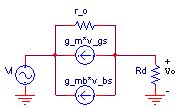
\includegraphics{schematics/ss_commongate_initial.PNG}
	\caption{Small signal model for the common gate circuit}
	\label{fig:ss_commongate_initial}
\end{figure}

\begin{figure}[h]
	\centering
		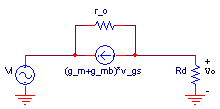
\includegraphics{schematics/ss_commongate_combine.PNG}
	\caption{Common gate small signal model with current sources combined}
	\label{fig:ss_commongate_combine}
\end{figure}

\begin{figure}[h]
	\centering
		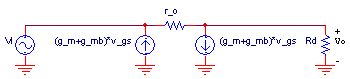
\includegraphics{schematics/ss_commongate_split.PNG}
	\caption{Common gate small signal model with current source split}
	\label{fig:ss_commongate_split}
\end{figure}

\begin{figure}[h]
	\centering
		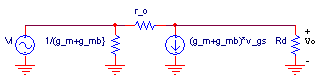
\includegraphics{schematics/ss_commongate_T_model.PNG}
		\caption{Common gate \textsl{T model}}
	\label{fig:ss_commongate_T_model}
\end{figure}

Assuming $r_{o} \to \infty$ we can determine the circuit's parameters by inspection:

\begin{equation}
G_{m} = g_{m} + g_{mb}
\end{equation}

\textcolor{red}{
\begin{equation}
R_{i} = \frac{1}{g_{m}+g_{mb}}
\end{equation}
}

\textcolor{red}{
\begin{equation}
R_{o} = R_{D}
\label{eq:common_gate_Ro}
\end{equation}
}

\textcolor{red}{
\begin{equation}
\frac{v_{o}}{v_{i}} = G_{m}R_{o} = (g_{m}+g_{mb})R_{D}
\end{equation}
}

\textcolor{red}{
\begin{equation}
\frac{i_{o}}{i_{i}} = G_{m}R_{i} = 1
\end{equation}
}

\section{Cascode}
\begin{center}
	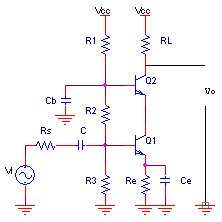
\includegraphics{schematics/cascode.PNG}
\end{center}
The cascode is a two transistor circuit that is actually a first stage common emitter/source driving a second stage common base/gate. To analyze the small signal voltage gain, we will approximate

\begin{equation}
i_{c1} = i_{e2} = \left(1+\frac{1}{\beta}\right)i_{c2}
\end{equation}

\noindent as

\begin{equation}
i_{c1} \approx i_{c2}
\end{equation}

\noindent This approximation is valid if $\beta_{0} >> 1$. Under this approximation 

\begin{equation}
g_{m1} = g_{m2}
\end{equation}

\noindent and

\begin{equation}
r_{\pi 1} = r_{\pi 2}
\end{equation}

\noindent We define these as $g_{m}$ and $r_{\pi}$, respectively. From the circuit configuration

\begin{equation}
v_{o} = -i_{c2}(R_{L}||r_{o}) \approx -i_{c1}(R_{L}||r_{o})
\end{equation}

\noindent and from the small signal model

\begin{equation}
i_{c1} = g_{m}v_{\pi 1} = g_{m}\frac{r_{\pi}}{r_{\pi}+ R'_{S}}v_{i}
\end{equation}

\noindent Substituting gives

\begin{equation}
v_{o} = -g_{m}\frac{r_{\pi}}{r_{\pi}+ R'_{S}}(R_{L}||r_{o})v_{i}
\end{equation}

\noindent Rearranging and noting that $\beta_{0} = g_{m}r_{\pi}$ we find

\textcolor{red}{
\begin{equation}
\frac{v_{o}}{v_{i}} = -\frac{\beta_{0} (R_{L}||r_{o})}{r_{\pi}+ R'_{S}}
\end{equation}
}

\par
This is the same voltage gain as the common emitter! Compared to the common emitter the cascode requires an extra transistor and additional bias circuitry, suffers from reduced signal swing (since $v_{o}$ is limited by two $v_{BE}$ drops rather than one), and offers the same voltage gain. Why would one ever use a cascode rather than just a common emitter? The key improvement of the cascode over the common emitter is its bandwidth. The resistance seen by $Q_{1}$'s $C_{\mu}$ for both the cascode and common emitter is

\begin{equation}
R'_{S}||r_{\pi} + (1 + g_{m}(R'_{S}||r_{\pi}))R_{LOAD}
\end{equation}

where $R_{LOAD}$ is the load resistance on the common emitter stage. By definition $R_{LOAD} = R_{L}$ for the common emitter, but $R_{LOAD} \approx \frac{1}{g_{m}}$ for the cascode ($C_{B}$ shorts $Q_{2}$'s base to AC ground so that the bias resistors do not affect $R_{LOAD}$). $R_{L}$ is usually much higher than $\frac{1}{g_{m}}$ (and it must be in order to acheive a high voltage gain) so this open circuit time constant is much smaller for the cascode than the common emitter, yet the cascode offers the same gain as the common emitter. The cascode is thus an extremely useful circuit for high gain while maintaining a high bandwidth, at the expense of signal swing.

\par
Since the first stage of the cascode is a common emitter, the input resistance $R_{i}$ is the same as (\ref{eq:common_emitter_Ri}):

\textcolor{red}{
\begin{equation}
R_{i} = r_{\pi} + (\beta_{0}+1)\left(\frac{r_{o} + \frac{R_{L}}{\beta_{0}+1}}{r_{o} + R_{L} + R_{E}}\right)R_{E}
\label{eq:cascode_Ri}
\end{equation}
}

\noindent and the output resistance $R_{o}$ is the same as (\ref{eq:common_base_Ro}):

\textcolor{red}{
\begin{equation}
R_{o} = R_{L}
\end{equation}
}

%\section{Super source follower (GHLM, p. 213)}

%\section{Common emitter/source (diode-connected load) (GHLM p. 284)}

\section{Differential pair}
The differential pair is a very common circuit in IC design.
It is rarely implemented using discrete components since it requires very good matching of components for good performance.
It is composed of two transistors whose emitters (in the bipolar case) or sources (in the MOS case) are tied together (some bipolar differential pairs connect the transistors' emitters through emitter degeneration resistors).
Bipolar differential pairs are often called emitter-coupled pairs and MOS differential pairs are often called source-coupled pairs.
The differential pair's topology can be used with a single-ended input (one of the transistors' bases or gates is biased to a particular voltage) and differential or single-ended output, or a differential input and differential or single-ended output.
The output voltage(s) are one or both of the transistors' collectors/drains.
If the differential pair is configured so that both the input and output are single-ended, the circuit is equivalent to a first stage emitter/source follower and second stage common base/gate:
the input is applied to the base (or gate) of one transistor (the other transistor's base or gate is tied to a bias voltage) and the output is taken from the collector (or drain) of the second transistor.
The differential input and output case is the most common, however, and such a circuit is a common input stage for an operational amplifier design.
Differential pairs configured with a differential input and output also have the benefit that they can be connected to each other in a cascade without using coupling capacitors between differential pair stages. \autocite[215]{analysis-design-analog-ics}

The differential pair is only linear for a narrow range of input voltages, but this limitation is usually unimportant since the differential pair is typically used as the input stage for high gain amplifiers (such as operational amplifiers), which prevents the input voltages from swinging outside the narrow linear range since the output voltage cannot swing above or below the supply voltages.
If the range of input voltages for which the differential pair is linear is too narrow for a particular application, the range can be increased by using emitter degeneration resistors.
The increase in the linear input voltage range, however, results in a decrease in the voltage gain of the differential pair. \autocite[216-218]{analysis-design-analog-ics}

Before analyzing the differential pair variants, a brief note on notation for common-mode and differential signals: if we define the voltage at one input as $v_{i1}$ and the voltage at the other input as $v_{i2}$, then the differential input is

\begin{equation}
v_{id} = v_{i1}-v_{i2}
\end{equation}

\noindent and the common-mode voltage is

\begin{equation}
v_{ic} = \frac{v_{i1}+v_{i2}}{2}
\end{equation}

The above equations can be inverted to define the input voltages $v_{i1}$ and $v_{i2}$ in terms of the differential voltage $v_{id}$ and common-mode voltage $v_{ic}$ \autocite[222]{analysis-design-analog-ics}:

\begin{equation}
v_{i1} = v_{ic}+\frac{v_{id}}{2}
\end{equation}

\begin{equation}
v_{i2} = v_{ic}-\frac{v_{id}}{2}
\end{equation}

By defining the input voltages as linear combinations of the differential and common-mode voltages, we can use superposition to analyze the differential pair's response to differential signals and its response to common-mode signals separately (as long as the input voltages are within the differential pair's linear range, since superposition is only valid for linear circuits). The output voltages can also be expressed in terms of the differential and common-mode output voltages in the same way.

\subsection{Differential pair with resistive load}
\begin{center}
	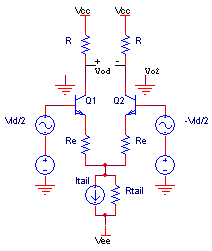
\includegraphics{schematics/differentialpair_resistorload.PNG}
\end{center}

The above differential pair is shown with a resistive load and with the optional emitter degeneration resistors $R_{E1}$ and $R_{E2}$.
The MOS version of the differential pair (the source-coupled pair) is the same but without the degeneration resistors and, of course, MOSFETs instead of $Q_{1}$ and $Q_{2}$.
The current source $I_{TAIL}$ and its output resistance $R_{TAIL}$ represent a Norton equivalent current source (usually composed of transistors, such as a current mirror), but the current source can simply consist of a resistor $R_{TAIL}$, in which $I_{TAIL} = 0$.
The bases (or gates) of the transistors are also biased to some voltage which is not necessarily equal to $GND$ (certainly not if $V_{EE} = GND$), but the bias voltages are usually equal so that $V_{B1} = V_{B2}$ (or $V_{G1} = V_{G2}$ in the MOS version).

%TODO: create figure for small signal model and minor rewrite of this paragraph
To determine the small signal differential behavior of this circuit set $I_{TAIL} = 0$ and use the bipolar hybrid-$\pi$ small signal model for the transistors (the MOS version of the circuit has a similar analysis, except with $r_{\pi} \to \infty$).
The voltage at the base of $Q_{1}$ is $\frac{v_{id}}{2}$ and the voltage at the base of $Q_{2}$ is $-\frac{v_{id}}{2}$, and the voltage at the collector of $Q_{1}$ is $\frac{v_{od}}{2}$ and the voltage at the collector of $Q_{2}$ is $-\frac{v_{od}}{2}$.
Both transistors act as voltage followers to the node that connects the two sides of the circuit (either the node that connects the emitter resistors or, if the emitter resistors are omitted, the node that connects the emitters).
Since this node is driven by equal and opposite input voltages its voltage is constant, and since its voltage is constant $R_{TAIL}$ can be shorted (which grounds the connecting node) without affecting the operation of the circuit. \autocite[226]{analysis-design-analog-ics}
Since the connecting node is grounded, the two sides of the differential pair are independent and are configured as common emitters!
The two independent sides are sometimes called \textit{differential half circuits}.
Using the above analysis of common emitters, we thus have a differential voltage gain of

\begin{equation}
\frac{v_{od}}{v_{id}} = -\frac{\beta_{F} (R \parallel r_{o})}{R_{S}' + r_{\pi}}
\end{equation}

where $r_{o}$ and $r_{\pi}$ are from the hybrid-$\pi$ small signal model and and $R_{S}'$ is defined as above. As before, we can often simplify the transfer function to

\begin{equation}
\frac{v_{od}}{v_{id}} \approx -g_m R
\label{eq:resistivediffpair_diff_gain_approx}
\end{equation}

The MOS version has a transfer function of

\begin{equation}
\frac{v_{od}}{v_{id}} = -g_{m}R
\end{equation}

since $r_{\pi} \to \infty$.

%TODO: create figure for small signal model for common-mode half circuits
A differential pair ideally has zero voltage gain for common-mode inputs.
To determine the actual small signal common-mode voltage gain use a similar approach as the differential voltage gain:
split the two sides of the circuit into two \textit{common-mode half circuits}.
To split the circuit replace $R_{TAIL}$ with two resistors in parallel with resistance $2R_{TAIL}$.
This does not modify the circuit since two identical resistors in parallel have an equivalent resistance of half the individual resistors.
The two sides are now combined only by a wire which connects the two $2R_{TAIL}$ resistors, but this wire carries no small signal current since both transistors are driven by identical input voltages ($v_{ic}$). \autocite[228]{analysis-design-analog-ics}
Consequently, the wire can be severed without affecting the circuit behavior and we have two \textit{common-mode half circuits} which are commom emitters with emitter degeneration resistances of $R_{E}+2R_{TAIL}$.
From (\ref{eq:commonemitter_transferfunction}) the common-mode voltage gain is thus

\begin{equation}
\frac{v_{oc}}{v_{ic}} = -\frac{g_{m}R}{1+g_{m}(R_{E}+2R_{TAIL})}
\label{eq:resistivediffpair_cm_gain}
\end{equation}

$R_{E}$ is usually much smaller than $2R_{TAIL}$ so the common-mode voltage gain is approximately

\begin{equation}
\frac{v_{oc}}{v_{ic}} \approx -\frac{g_{m}R}{1+2g_{m}R_{TAIL}}
\label{eq:resistivediffpair_cm_gain_approx}
\end{equation}

Using the approximate differential voltage gain (\ref{eq:resistivediffpair_diff_gain_approx}) divided by the the approximate common-mode voltage gain (\ref{eq:resistivediffpair_cm_gain_approx}) gives a good approximation of the common-mode rejection ratio CMRR, which is

\textcolor{red}{
\begin{equation}
\text{CMRR} \approx 1+2g_m R_{TAIL}
\label{eq:resistivediffpair_CMRR}
\end{equation}
}

The CMRR is strongly dependent on the value of $R_{TAIL}$ so the use of a good current source (which has an ideally infinite Norton equivalent resistance) yields a high CMRR.

The differential pair shown uses \textit{npn} transistors, but $Q_{1}$ and $Q_{2}$ can also be \textit{pnp} transistors.
If \textit{pnp} transistors are used the only difference is that $I_{TAIL}$ is sourced from $V_{CC}$ rather than sinking into $V_{EE}$.
The same is true of the MOS version of the differential pair -- PMOS transistors can be used instead of NMOS with the same change in $I_{TAIL}$.

\subsection{Differential pair with active load (GHLM, p. 278, 288)}
\begin{center}
	\includegraphics{schematics/differentialpair_activeload.PNG}
\end{center}
The gain of the differential pair can be increased by using an active load. $Q_{3}$ and $Q_{4}$ form a current mirror (since $Q_{3}$ is diode connected) so that $I_{TAIL}$ is split evenly and $I_{C1} = I_{C2}$. Unfortunately, the circuit is no longer symmetrical since only $Q_{3}$ is diode connected and as a result the \textsl{differential half circuit} approach used above cannot be employed.

%\subsection{Rail-to-rail differential pair (Op Amps for Everyone, p. 386)}

%\section{Wideband amplifier (my design)}
\chapter{Voltage Sources and References}
Voltage sources are circuits designed to maintain a constant voltage and supply a load current to other circuitry.
Voltage references also maintain a constant voltage for other circuitry (for example, to bias a one input of a comparator so that the comparator's output is high when its input is at a higher voltage than the voltage reference and low otherwise).
Unlike voltage sources, however, voltage references are usually not required to supply a significant load current.
Ideally, the voltage output $v_{O}$ of voltage references and sources does not vary with the load current and $v_{O}$ has no \AC component (it is a pure \DC voltage).
In practice, higher load currents often cause $v_{O}$ to decrease slightly because the voltage reference/source has a nonzero output resistance $R_{o}$.
If the input voltage is $v_{I}$ and the load current $i_{L}$, then the output voltage is

\begin{equation}
v_{O} = v_{I} - i_{L}R_{o}
\end{equation}

It is crucial, therefore, for a voltage source to have a low $R_{o}$.
Voltage references should also have a low $R_{o}$, but they do not need to supply larger load currents so $v_{O} \approx v_{I}$ even if $R_{o}$ is significant.
Also in practice, \AC noise is present in the output.
One way to minimize \AC noise is to add a low pass filter after the voltage source/reference to help remove the high frequency noise.
However, the low pass filter will affect $R_{o}$.
%http://en.wikipedia.org/wiki/Image:Op-amp_current_source_with_pass_transistor.png
\section{Resistor divider}
\begin{center}
	\includegraphics{schematics/resistordivider.PNG}
\end{center}
The resistor divider is the simplest voltage source or reference possible. Its transfer function (unloaded) can be determined by inspection:

\begin{equation}
v_{O} = \frac{R_2 v_{I}}{R_1 + R_2}
\end{equation}

When loaded by a resistance $R_{L}$, the transfer function is the same but with $R_2$ replaced by $R_2 \parallel R_{L}$. Specifically,

\textcolor{red}{
\begin{equation}
v_{O} = \frac{R_2 R_{L}v_{I}}{R_1(R_2 + R_{L})+R_2 R_{L}}
\end{equation}
}

The output resistance $R_{o}$ is also easy to determine -- with $v_{I} = 0$ the two resistors are in parallel looking into the output:

\textcolor{red}{
\begin{equation}
R_{o} = \frac{R_1 R_2}{R_1 + R_2}
\end{equation}
}

$R_{o}$ is usually quite high since $R_1$ and $R_2$ must be large enough that the current drawn by the circuit is not unnecessarily high. Consequently, the simple resistor divider is a poor voltage source and is often only used as a voltage reference.

\section{Resistor divider with emitter/source follower}
\begin{center}
	\includegraphics{schematics/resistordivider_emitterfollower.PNG}
\end{center}

One way to improve $R_{o}$ of the resistor divider is to connect an emitter/source follower to the output.
An emitter/source follower has a high input resistance so that the load current seen by the resistor divider is low, but it also has a low output resistance.
The drawback is that $v_{O}$ is lower by approximately $v_{BE}$ or $v_{GS}$ due to the transistor.
More specifically, $v_{O}$ is dependent on the load current $i_{L}$ since

\begin{equation}
v_{O} = i_{L}R_{L}
\end{equation}

For an emitter follower, the relationship between $i_{L}$ and $v_{BE}$ is given by (\ref{eq:bipolarIc}). Since

\begin{equation}
i_{L} = i_{E} = \frac{\beta_{F}+1}{\beta_{F}}i_{C}
\end{equation}

we can use (\ref{eq:bipolarIc}) to find $v_{BE}$ in terms of $i_{L}$:

\begin{equation}
v_{BE} = V_{th}\ln\left(\frac{\beta_{F}i_{L}}{(\beta_{F}+1)I_{S}}\right)
\end{equation}

The transfer function is therefore

\textcolor{red}{
\begin{equation}
v_{O} = \frac{R_2 v_{I}}{R_1 + R_2} - V_{th}\ln\left(\frac{\beta_{F}i_{L}}{(\beta_{F}+1)I_{S}}\right)
\end{equation}
}

The output resistance $R_{o}$ is simply that of an emitter follower, given by (\ref{eq:emitter_follower_Ro}).
In terms of the above circuit it is

\textcolor{red}{
\begin{equation}
R_{o} = \frac{(R_{1}||R_{2})+r_{\pi}}{\beta_{F}+1}||r_{o}
\end{equation}
}

If a source follower is used instead then the relationship between $i_{L}$ and $v_{GS}$ is given by (\ref{eq:activeId}).
For the MOS transistor

\begin{equation}
i_{L} = i_{D}
\end{equation}

so we can solve for $v_{GS}$ in (\ref{eq:activeId}) to find $v_{GS}$ in terms of $i_{L}$:

\begin{equation}
v_{GS} = V_{t} + \sqrt{\frac{L}{W}\frac{2I_{D}}{\mu_{n}C_{ox}}\left(1+\frac{V_{DS}}{V_{A}}\right)}
\end{equation}

The transfer function is therefore

\textcolor{red}{
\begin{equation}
v_{O} = \frac{R_{2}v_{I}}{R_{1}+R_{2}} - \left(V_{t} + \sqrt{\frac{L}{W}\frac{2I_{D}}{\mu_{n}C_{ox}}\left(1+\frac{V_{DS}}{V_{A}}\right)}\right)
\end{equation}
}

and the output resistance $R_{o}$ is the same as (\ref{eq:sourcefollower_Ro}):

\textcolor{red}{
\begin{equation}
R_{o} = \frac{1}{g_m + g_{mb}+\frac{1}{r_o}+\frac{1}{R_{L}}}
\end{equation}
}

\section{Resistor divider with operational amplifier buffer}
\begin{center}
	\includegraphics{schematics/resistordivider_opampbuffer.PNG}
\end{center}
The best way to improve the output resistance of $R_{o}$ of the resistor divider is to use an operational amplifier buffer on the output (although the use of a full operational amplifier may be unnecessary or undesirable).
Unlike the emitter/source follower, the output voltage is not lowered by a $v_{BE}$ (or $v_{GS}$) drop and is simply

\textcolor{red}{
\begin{equation}
v_{O} = \frac{R_2 v_{I}}{R_1 + R_2}
\end{equation}
}

The output resistance $R_{o}$ is simply the operational amplifier's $R_{o}$.

\section{Zener diode regulator}
\begin{center}
	\includegraphics{schematics/zenerdiode_regulator.PNG}
\end{center}

The Zener diode regulator relies on a Zener diode's reverse-bias breakdown voltage -- the reverse-bias voltage $V_{Z}$ at which a Zener diode begins to conduct current.
The Zener diode has a low impedance at $V_{Z}$ so the reverse-bias voltage remains mostly constant even over a wide range of reverse current through the diode.
The series resistor $R_1$ limits the current through the diode.
As long as $V_{I} > V_{Z}$ and the current through the diode is nonzero

\textcolor{red}{
\begin{equation}
v_{O} = V_{Z}
\end{equation}
}

The output resistance $R_{o}$ is approximately the (low) resistance of the Zener diode in reverse breakdown, $R_{Z}$, since generally $R_{1} \gg R_{Z}$ and

\textcolor{red}{
\begin{equation}
R_{o} = R_1 \parallel R_{Z} \approx R_{Z}
\end{equation}
}

As with the resistor divider, the simple Zener diode regulator can be improved by adding an emitter/source follower or operational amplifier buffer to the output.
In this case, the emitter/source follower or operational amplifier buffer help ensure that the reverse-bias voltage across the diode remains greater than the diode's reverse-bias breakdown voltage.

\section{$V_{BE}$ multiplier}
\begin{center}
	\includegraphics{schematics/vbe_multiplier.PNG}
\end{center}

The $V_{BE}$ multiplier requires a bipolar transistor with a high $\beta_{F}$.
If $\beta_{F} \gg 1$ then $I_{B}$ (the base current into the transistor) is negligible.
With that assumption the current $I$ through $R_1$ is equal to the current through $R_2$.
Since the current through the resistors is nearly equal

\begin{equation}
V_{O} = I(R_1 + R_2)
\end{equation}

The voltage across $R_2$ is equal to $V_{BE}$ so

\begin{equation}
I = \frac{V_{BE}}{R_2}
\end{equation}

and thus

\textcolor{red}{
\begin{equation}
V_{O} = V_{BE}\left(1+\frac{R_1}{R_2}\right)
\label{eq:vbe_multiplier_Vo}
\end{equation}
}

To choose the appropriate $I_{I}$, make sure $Q_1$ is in the forward active region (so that $\beta_{F} \gg 1$):

\begin{equation}
V_{BE1} > 0
\end{equation}

and

\begin{equation}
V_{CE1} > V_{CE(\text{sat})}
\end{equation}

\section{Widlar bandgap reference}
\begin{center}
	\includegraphics{schematics/Widlar_bandgap.PNG}
\end{center}
The Widlar bandgap reference circuit has two stable operating points but only one desirable operating point, so a start-up circuit (not shown above) is required to ensure that the circuit reaches the desirable operating point.
Assuming the circuit is in the desired stable operating point,

\begin{equation}
V_{O} = V_{BE3} + V_{R2}
\label{eq:Widlar_bandgap_Vo_basic}
\end{equation}

where $V_{R2}$ is the voltage across $R_2$.
The current through $R_2$ is approximately equal to $R_3$ if $Q_2$'s $\beta_{F} \gg 1$, in which case

\begin{equation}
V_{R2} = I_{C2}R_2 = \frac{R_2}{R_3}V_{R3}
\label{eq:Widlar_bandgap_Vr2_wrt_Vr3}
\end{equation}

and the voltage across $R_3$ is

\begin{equation}
V_{R3} = V_{BE1} - V_{BE2} = V_{T}\ln\left(\frac{I_{C1}}{I_{C2}}\frac{I_{S2}}{I_{S1}}\right)
\end{equation}

The ratio of $I_{C1}$ to $I_{C2}$ is determined by the ratio of $R_2$ to $R_1$, so %TODO: why?????????

\begin{equation}
V_{R3} = V_{T}\ln\left(\frac{R_2}{R_1}\frac{I_{S2}}{I_{S1}}\right)
\label{eq:Widlar_bandgap_Vr3_R}
\end{equation}

Substituting (\ref{eq:Widlar_bandgap_Vr3_R}) into (\ref{eq:Widlar_bandgap_Vr2_wrt_Vr3}),

\begin{equation}
V_{R2} = \frac{R_2}{R_3}V_{T}\ln\left(\frac{R_2}{R_1}\frac{I_{S2}}{I_{S1}}\right)
\label{eq:Widlar_bandgap_Vr2_R}
\end{equation}

Substituting (\ref{eq:Widlar_bandgap_Vr2_R}) into (\ref{eq:Widlar_bandgap_Vo_basic}),

\textcolor{red}{
\begin{equation}
V_{O} = V_{BE3} + \frac{R_2}{R_3}\ln\left(\frac{R_2}{R_1}\frac{I_{S2}}{I_{S1}}\right)V_{T}
\end{equation}
}

The base-emitter voltage is inversely proportional to temperature and the voltage across $R_2$ is \ac{ptat} due to the temperature dependence of $V_{T}$, so an appropriate choice of the multiplicative factor to $V_{T}$ cancels the temperature coefficent for $V_{O}$ at the desired temperature. The multiplicative factor is determined by three ratios: $R_2$ to $R_3$, $R_2$ to $R_1$, and $I_{S2}$ to $I_{S1}$. \autocite[322-323]{analysis-design-analog-ics}

%\section{Improved Widlar bandgap reference (GHLM p. 323)}

%\section{Brokaw bandgap reference}
%http://en.wikipedia.org/wiki/Brokaw_bandgap_reference

%\section{Op amp voltage regulator (p.230)}
\chapter{Current Mirrors and Current Sources}
Current mirrors are circuits that are used primarily in integrated circuits to bias other circuit elements or act as active loads (such as in the actively loaded differential pair).
They can also be used to sense a current signal in a circuit and mirror (or multiply) it elsewhere to be acted upon or measured by other circuitry.
Current mirrors are commonly constructed out of bipolar transistors or MOSFETs.
They do not find much use outside of integrated circuits because they require transistor matching and sizing (which is easily accomplished when transistors are manufactured in the same \ac{ic} process) and because they usually require less die area than a resistor to provide a particular bias current.

Current mirrors have several important parameters, including current gain, output resistance $R_{o}$ (ideally infinite), systematic gain error $\epsilon$ (deviation from the ideal current gain), and minimum input and output voltages.

\section{Simple current mirror (Bipolar and MOS)}
\begin{center}
	\includegraphics{schematics/simplecurrentmirror.PNG}
\end{center}
This is the most basic form of current mirror.
The two transistors have the same $V_{BE}$ drop (or $V_{GS}$ in the MOS case) since their bases/gates are tied together and their emitters/sources are both connected to a supply voltage or ground.
$Q_1$/$M_1$ is diode connected, which means that the base/gate is shorted to the collector/drain.
\subsection{Bipolar}
For the bipolar case,

\begin{equation}
V_{BE1} = V_{T}\ln\frac{I_{C1}}{I_{S1}} = V_{BE2} = V_{T}\ln\frac{I_{C2}}{I_{S2}}
\end{equation}

(where $I_{S1}$ and $I_{S2}$ are the transistors' saturation currents and $V_{T} = \frac{kT}{q}$ is the thermal voltage).
Canceling terms on both sides, we see that

\begin{equation}
I_{O} = I_{C2} = \frac{I_{S2}}{I_{S1}}I_{C1}
\end{equation}

Assuming $Q_1$ and $Q_2$ have the same $\beta_{F}$, we also know that

\begin{equation}
I_{I} = I_{C1} + \frac{I_{C1}}{\beta_{F}} + \frac{I_{C2}}{\beta_{F}}
\end{equation}

Solving for $I_{C1}$ and substituting we find

\textcolor{red}{
\begin{equation}
I_{O} = \left(\frac{1}{1+\frac{1+(I_{S2}/I_{S1})}{\beta_{F}}}\right)\left(\frac{I_{S2}}{I_{S1}}\right)I_{I}
\label{eq:simplecurrentmirror}
\end{equation}
}

If $I_{S1} = I_{S2}$ the above equation simplifies to

\textcolor{red}{
\begin{equation}
I_{O} = \left(\frac{1}{1 + \frac{2}{\beta_{F}}}\right)I_{I}
\label{eq:simplecurrentmirror_Is_equal}
\end{equation}
}

If $\beta_{F}$ is large the above equations simplify to

\textcolor{red}{
\begin{equation}
I_{O} \approx \frac{I_{S2}}{I_{S1}}I_{I}
\label{eq:simplecurrentmirror_Beta_large}
\end{equation}
}

A bipolar transistor's saturation current $I_{S}$ is proportional to its emitter area so the current gain of the current mirror can be any rational number -- unity, or less than or greater than unity.
The current mirror gets its name from the fact that $I_{C1}$ is mirrored to $I_{C2}$ when the current gain is unity.
One way to set the emitter area ratio when the current gain is not unity is to connect $M$ unit bipolar transistors in parallel as $Q_2$ and $N$ unit bipolar transistors in parallel as $Q_1$ for an emitter area ratio of $M/N$.

The above approximation is the ideal current gain of the current mirror.
Clearly the approximation is not realized (at least in the bipolar case) due to finite $\beta_{F}$.
However, the above analysis neglected the dependence of the transistors' collector currents on the collector-emitter voltage.
Taking into account this dependence as well, the transfer function is

\textcolor{red}{
\begin{equation}
I_{O} = \frac{1+\frac{V_{CE2}-V_{CE1}}{V_{A}}}{1+\frac{1+I_{S2}/I_{S1}}{\beta_{F}}}\frac{I_{S2}}{I_{S1}}I_{I}
\label{eq:fullsimplecurrentmirror}
\end{equation}
}

where $V_{A}$ is the Early voltage.
The systematic gain error is therefore

\textcolor{red}{
\begin{equation}
\epsilon = \frac{1+\frac{V_{CE2}-V_{CE1}}{V_{A}}}{1+\frac{1+I_{S2}/I_{S1}}{\beta_{F}}}-1
\label{eq:simplecurrentmirror_sysgainerr}
\end{equation}
}

and is thus caused by both finite $\beta_{F}$ and finite output resistance $r_{o} = \frac{V_{A}}{I_{C}}$.

The input voltage $V_{I}$ is simply

\textcolor{red}{
\begin{equation}
V_{I} = V_{CE1} = V_{BE1}
\label{eq:simplecurrentmirror_Vi}
\end{equation}
}

since $Q_1$ is diode connected, and the minimum output voltage is

\textcolor{red}{
\begin{equation}
V_{O(\text{min})} = V_{CE2(\text{sat})}
\label{eq:simplecurrentmirror_Vo}
\end{equation}
}

since $Q_2$ must remain in the forward active region.

Another important characteristic of a current mirror is its output resistance.
Ideally, its output resistance is infinite since the current mirror is a current source.
Of course, no real current mirror has an infinite resistance -- in reality the output resistance is dependent on the output current.
For the bipolar case the output resistance \autocite[255-256]{analysis-design-analog-ics} $R_{o}$ is

\textcolor{red}{
\begin{equation}
R_{o} = r_{o2} = \frac{V_{A}}{I_{C2}} = \frac{V_{A}}{I_{O}}
\label{eq:simplecurrentmirror_Ro}
\end{equation}
}

\subsection{MOS}
The MOS current mirror has the same topology as the bipolar current mirror, and its analysis is similar. The MOSFETs must be biased so that $V_{GS} > V_{t}$ (where $V_{t}$ is the threshold voltage).
Using the characteristic equation of a MOSFET in the active region and noting that $V_{GS1} = V_{GS2}$ we see that

\begin{equation}
V_{GS1} = V_{t} + \sqrt{\frac{2I_{D1}}{k'(W/L)_{1}}} = V_{GS2} = V_{t} + \sqrt{\frac{2I_{D2}}{k'(W/L)_{2}}}
\end{equation}

Canceling terms on both sides we see that

\textcolor{red}{
\begin{equation}
I_{O} = \frac{(W/L)_{2}}{(W/L)_{1}}I_{D1} = \frac{(W/L)_{2}}{(W/L)_{1}}I_{I}
\label{eq:MOSsimplecurrentmirror}
\end{equation}
}

As with the bipolar case, the current gain can be set to any rational number by sizing the MOSFETs appropriately. \autocite[258]{analysis-design-analog-ics}

Similar to the bipolar case, the above analysis neglects the slight dependence of a MOSFET's $I_{D}$ to its $V_{DS}$.
If we take this dependency into account, the transfer function is

\textcolor{red}{
\begin{equation}
I_{O} = \frac{(W/L)_{2}}{(W/L)_{1}}I_{I}\left(1+\frac{V_{DS2}-V_{DS1}}{V_{A}}\right)
\label{eq:MOSsimplecurrentmirrorfull}
\end{equation}
}

where $V_{A} = 1/\lambda$, the MOS equivalent of the Early voltage.
The systematic gain error is therefore

\textcolor{red}{
\begin{equation}
\epsilon = \frac{V_{DS2}-V_{DS1}}{V_{A}}
\label{eq:MOSsimplecurrentmirror_sysgainerr}
\end{equation}
}

The input voltage $V_{I}$ is simply

\textcolor{red}{
\begin{equation}
V_{I} = V_{DS1} = V_{GS1}
\label{eq:MOSsimplecurrentmirror_Vi}
\end{equation}
}

since $M_1$ is diode connected, the minimum output voltage $V_{O(min)}$ is

\textcolor{red}{
\begin{equation}
V_{O(min)} = V_{ov2} = \sqrt{\frac{2I_{O}}{(W/L)_{2}k}}
\label{eq:MOSsimplecurrentmirror_Vo}
\end{equation}
}

where $V_{ov}$ is the overdrive voltage above $V_{t}$ (i.e. $V_{GS} = V_{t} + V_{ov}$).
The output resistance $R_{o}$ is \autocite[256, 259]{analysis-design-analog-ics}

\textcolor{red}{
\begin{equation}
R_{o} = r_{o2} = \frac{1}{\lambda I_{D2}} = \frac{1}{\lambda I_{O}}
\label{eq:MOSsimplecurrentmirror_Ro}
\end{equation}
}

For all current mirrors, the current source $I_{I}$ can be implemented by a number of devices.
The simplest is a resistor.
In that case, use the desired $I_{C1}$ and $I_{C2}$ (or $I_{D1}$ and $I_{D2}$ in the MOS case) to determine $V_{BE1} = V_{CE1}$ (or $V_{GS1} = V_{DS1}$) from the transistor's characteristic equation, and then use \ac{kvl} to find $R = \frac{V_{CC} - V_{CE1}}{I_{C1}}$ (or $R = \frac{V_{DD} - V_{DS1}}{I_{D1}}$).

One very useful aspect of current mirrors is that $Q_1$ (or $M_1$) can be used to generate as many output currents as needed;
for each output current simply add another transistor whose base (or gate) is tied to the base (or gate) of $Q_1$ (or $M_1$) and whose emitter (or source) is tied to the emitter (or source) of $Q_1$ (or $M_1$).
The additional output currents flow into the collectors (or drains) of these additional transistors and, by choosing the emitter areas or W/L ratios appropriately, the additional output currents can all have different values.

\section{Simple current mirror with $\beta_{F}$ helper}
\begin{center}
	\includegraphics{schematics/currentmirrorbetahelper.PNG}
\end{center}
For the bipolar simple current mirror we assumed $\beta_{F}$ was large enough that we could approximate $I_{O} = \frac{I_{S2}}{I_{S1}}I_{I}$ (the MOS current mirror has an approximately infinite $\beta_{F}$ so it is not applicable here).
To make the current mirror better approximate this ideal relationship (especially if $\beta_{F}$ is relatively small) an additional transistor is added. In this case, \ac{kcl} at $Q_1$'s collector yields

\begin{equation}
I_{I} = I_{C1} + I_{B2}
\label{eq:currentmirrorbetahelper_KCL}
\end{equation}

To find $I_{B2}$ note that

\begin{equation}
I_{E2} = \frac{I_{C1}}{\beta_{F}} + \frac{I_{C3}}{\beta_{F}}
\label{eq:currentmirrorbetahelper_Ie2}
\end{equation}

and

\begin{equation}
I_{B2} = \frac{I_{E2}}{\beta_{F} + 1}
\label{eq:currentmirrorbetahelper_Ib2}
\end{equation}

so substituting (\ref{eq:currentmirrorbetahelper_Ie2}) into (\ref{eq:currentmirrorbetahelper_Ib2}) we have

\begin{equation}
I_{B2} = \frac{I_{C1} + I_{C3}}{\beta_{F}(\beta_{F} + 1)}
\label{eq:currentmirrorbetahelper_Ib2_2}
\end{equation}

Also,

\begin{equation}
I_{C1} = \frac{I_{S1}}{I_{S3}}I_{C3} = \frac{I_{S1}}{I_{S3}}I_{O}
\label{eq:currentmirrorbetahelper_Ic1}
\end{equation}

as before.
Substituting (\ref{eq:currentmirrorbetahelper_Ib2_2}) and (\ref{eq:currentmirrorbetahelper_Ic1}) into (\ref{eq:currentmirrorbetahelper_KCL}) we see

\begin{equation}
I_{I} = \frac{I_{S1}}{I_{S3}}I_{O} + \frac{I_{C1} + I_{C3}}{\beta_{F}(\beta_{F} + 1)} = \frac{I_{S1}}{I_{S3}}I_{O} + \frac{\frac{I_{S1}}{I_{S3}}I_{O} + I_{O}}{\beta_{F}(\beta_{F} + 1)}
\end{equation}

Solving for $I_{O}$ we see that

\textcolor{red}{
\begin{equation}
I_{O} = \left(\frac{1}{1 + \frac{1 + (I_{S3}/I_{S1})}{\beta_{F}(\beta_{F} + 1)}}\right)\frac{I_{S3}}{I_{S1}}I_{I}
\label{eq:currentmirrorbetahelper}
\end{equation}
}

which is the same as the simple current mirror except for the extra $\beta_{F} + 1$ term which multiplies with $\beta_{F}$.

The approximation that

\textcolor{red}{
\begin{equation}
I_{O} \approx \frac{I_{S3}}{I_{S1}}I_{I}
\label{eq:currentmirrorbetahelper_approx}
\end{equation}
}

is even better with the $\beta_{F}$ helper.
Since a MOSFET has $\beta_{F} \approx \infty$ the base current error can be completely eliminated if a MOSFET is used as the $\beta_{F}$ helper transistor.

The $\beta_{F}$ helper does not significantly alter the output resistance $R_{o}$ or the minimum output voltage $V_{O(min)}$, but the input voltage is created by the $V_{BE}$ drop of the $\beta_{F}$ helper (or $V_{GS}$ if the $\beta_{F}$ helper is a MOSFET).
Assuming a bipolar $\beta_{F}$ helper, the input voltage is thus

\textcolor{red}{
\begin{equation}
V_{I} = V_{BE1} + V_{BE2}
\label{eq:currentmirrorbetahelper_Vi}
\end{equation}
}

The current mirror with $\beta_{F}$ helper is also better when multiple outputs are needed.
For every extra output another transistor's base must be connected to the base of $Q_{1}$, which increases the gain error due to the finite $\beta_{F}$.
The $\beta_{F}$ helper reduces this gain error for each output by $\beta_{F}+1$.
The cost of the $\beta_{F}$ helper is that $V_{CE1}$ has an extra $V_{BE}$ drop (now $V_{CE1} = V_{BE1}+V_{BE2}$), which can be a limitation if $V_{CC}$ is low. \autocite[261-262]{analysis-design-analog-ics}

\section{Simple current mirror with $\beta_{F}$ helper and degeneration}
\begin{center}
	\includegraphics{schematics/currentmirror_betahelper_degeneration.PNG}
\end{center}

\subsection{Bipolar}
Emitter degeneration improves a current mirror by providing better matching between the input current $I_{I}$ and output current $I_{C3}$, and by increasing the mirror's output resistance $R_{o}$ from $R_{o} = r_{o3}$ to

\textcolor{red}{
\begin{equation}
R_{o} \approx r_{o3}(1+g_{m}R_{3})
\end{equation}
}

The increased $R_{o}$ not only makes the current mirror behave more like an ideal current source (which has an infinite $R_{o}$), but it decreases the systematic gain error $\epsilon$ since a finite $R_{o}$ contributes to $\epsilon$.
A simple current mirror with a $\beta_{F}$ helper and emitter degeneration thus has a systematic gain error of

\textcolor{red}{
\begin{equation}
\epsilon = \frac{1+\frac{V_{CE2}-V_{CE1}}{V_{A}(1+\frac{I_{C3}R_{3}}{V_{T}})}}{1+\frac{1+I_{S2}/I_{S1}}{\beta_{F}(\beta_{F}+1)}}-1
\end{equation}
}

The drawback of emitter degeneration is, of course, the increase in the minimum input and output voltages by approximately $I_{I}R_{1}$ and $I_{O}R_{3}$, respectively.
The transfer function is easily expressed in implicit form by using \ac{kvl} and noting that $I_{I} = I_{C1}$ and $I_{O} = I_{C3}$:

\begin{equation}
I_{I}R_{1}+V_{T}\ln\frac{I_{I}}{I_{S1}} = I_{O}R_{3}+V_{T}\ln\frac{I_{O}}{I_{S3}}
\end{equation}

so

\begin{equation}
I_{O} = \frac{1}{R_{3}}\left(I_{I}R_{1} + V_{T}\ln\frac{I_{I}I_{S3}}{I_{O}I_{S1}}\right)
\end{equation}

Given a desired input/output current ratio $\frac{I_{O}}{I_{I}}$, $I_{O}$ can be set by choosing the appropriate resistor ratio $\frac{R_{1}}{R_{3}}$ and/or sizing the transistors appropriately (which changes $\frac{I_{S3}}{I_{S1}}$).

The emitter degeneration resistors are limited by the supply voltage $V_{CC}$ since the input voltage $V_{I}$ is

\textcolor{red}{
\begin{equation}
V_{I} = I_{E1}R_{1}+V_{BE1}+V_{BE2} = \left(\frac{1}{\beta_{F}}+1\right)I_{C1}R_{1}+V_{BE1}+V_{BE2}
\end{equation}
}

and the minimum output voltage $V_{O(min)}$ is

\textcolor{red}{
\begin{equation}
V_{O(\text{min})} = I_{E3}R_{3}+V_{CE3(\text{sat})} = \left(\frac{1}{\beta_{F}}+1\right)I_{C3}R_{3}+V_{CE3(\text{sat})}
\end{equation}
}

and both must be less than $V_{CC}$.
\subsection{MOS}
Source degeneration is not as commonly used as emitter degeneration because matching of MOS current mirrors can be improved by increasing the MOS transistors' gate areas, and $R_{O}$ can be increased by increasing the transitors' channel length.
Nonetheless, the analysis for the bipolar current mirror with $\beta_{F}$ helper and emitter degeneration can be applied to a MOS variant easily. \autocite[262-263]{analysis-design-analog-ics}

\section{Cascode current mirror (Bipolar and MOS)}
\begin{center}
	\includegraphics{schematics/cascodecurrentmirror.PNG}
\end{center}

\subsection{Bipolar}
A cascode current mirror significantly increases $R_{o}$.
Transistors $Q_1$ and $Q_3$ in the above schematic form a simple current mirror (which may also include emitter degeneration).
$Q_2$ is in a common base configuration and transfers $I_{C1}$ to $I_{O} = I_{C2}$, and $Q_4$ is connected as a diode to properly bias $Q_2$ and ensure it is in the forward active region.
$R_{o}$ is greatly increased over the simple current mirror (even with emitter degeneration) because the ``emitter resistance'' is the resistance looking into the collector of $Q_1$.
Small-signal analysis reveals that

\textcolor{red}{
\begin{equation}
R_{o} \approx \frac{\beta_{F} r_{o2}}{2}
\end{equation}
}

($R_{o}$ is reduced by half due to the simple current mirror formed by $Q_1$ and $Q_3$, which diverts half of $I_{O} = I_{C2}$ through $r_{\pi 2}$). \autocite[264]{analysis-design-analog-ics}
The drawback of the cascode current mirror versus a simple current mirror is that the input voltage is increased to

\textcolor{red}{
\begin{equation}
V_{I} = V_{BE3} + V_{BE4}
\end{equation}
}

and the minimum output voltage is increased to

\textcolor{red}{
\begin{equation}
V_{O(\text{min})} = V_{BE1} + V_{CE(\text{sat})}
\end{equation}
}

so that both $Q_1$ and $Q_2$ are in the forward active region.

To derive the cascode current mirror's transfer function we note that

\begin{equation}
I_{E4} = I_{C3}+\frac{2I_{C3}}{\beta_{F}}
\label{eq:cascodecurrentmirror_Ie4}
\end{equation}

\begin{equation}
I_{I} = I_{E4}+\frac{I_{C2}}{\beta_{F}}
\label{eq:cascodecurrentmirror_Ii}
\end{equation}

\begin{equation}
I_{O} = I_{C2} = \frac{\beta_{F}}{\beta_{F} + 1}I_{C3}
\label{eq:cascodecurrentmirror_Io}
\end{equation}

Substituting (\ref{eq:cascodecurrentmirror_Ie4}) into (\ref{eq:cascodecurrentmirror_Ii}) we find

\begin{equation}
I_{I} = I_{C3} + \frac{2I_{C3}}{\beta_{F}} + \frac{I_{C3}}{\beta_{F} + 1}
\label{eq:cascodecurrentmirrorIi_2}
\end{equation}

Rearranging (\ref{eq:cascodecurrentmirrorIi_2}) to solve for $I_{C3}$ and substituting the result into (\ref{eq:cascodecurrentmirror_Io}), we see that

\textcolor{red}{
\begin{equation}
I_{O} = \frac{\beta_{F}}{\beta_{F} + 1}\frac{I_{I}}{1+ \frac{2}{\beta_{F}} + \frac{1}{\beta_{F} + 1}} = I_{I}\left(1-\frac{4\beta_{F} + 2}{\beta_{F}^{2} + 4\beta_{F} + 2}\right)
\end{equation}
}

The systematic gain error is clear from the above transfer function:

\textcolor{red}{
\begin{equation}
\epsilon = -\frac{4\beta_{F} +  2}{\beta_{F}^{2} + 4\beta_{F} + 2} \approx -\frac{4}{\beta_{F} + 4}
\end{equation}
}

and is generally greater than $\epsilon$ for a simple current mirror.

\subsection{MOS}
The MOS version of the cascode current mirror does not have the same finite $\beta_{F}$ problems as the bipolar version.
Consequently, a MOS cascode current mirror can be made to have as high an output resistance as needed by increasing the number of stacked cascode MOSFETs (provided the increase in the minimum input and output voltages required by the additional cascodes is acceptable).
The output resistance for a single MOS cascode current mirror is

\textcolor{red}{
\begin{equation}
R_{o} = r_{o2}(1+(g_{m2}+g_{mb2})r_{o1})+ r_{o1}
\end{equation}
}

and each cascode increases $R_{o}$ by approximately a factor of $1+g_{m}r_{o}$ (although in practice $R_{o}$ is limited by parasitic leakage paths as the number of cascodes increases). \autocite[263-268]{analysis-design-analog-ics}
%TODO: Add info on Vo(min) and Vi

\section{Wilson current mirror}
\begin{center}
	\includegraphics{schematics/wilsoncurrentmirror.PNG}
\end{center}

\subsection{Bipolar}
The Wilson current mirror is a slight variation on the cascode current mirror.
$Q_4$ is removed and $Q_1$ is the only diode connected transistor, which ensures that

\begin{equation}
V_{CE3} = V_{BE1} + V_{BE2} \approx 2V_{BE}
\end{equation}

Bipolar Wilson current mirrors are designed to minimize the systematic gain error $\epsilon$ in cascode current mirrors caused by finite $\beta_{F}$ by using negative feedback through $Q_1$ to activate $Q_3$, which increases $R_{o}$ and reduces the base current error.

To find the transfer function, first use \ac{kcl} at $Q_1$'s collector to find

\begin{equation}
I_{E2} = I_{C1} + I_{B1} + I_{B3} = I_{C1}\left(1+\frac{1}{\beta_{F}}\right) + \frac{I_{C3}}{\beta_{F}}
\end{equation}

Approximating $I_{C1} = I_{C3}$, we see that

\begin{equation}
I_{E2} = I_{C1}\left(1+\frac{2}{\beta_{F}}\right)
\end{equation}

It follows that

\begin{equation}
I_{O} = I_{C2} = I_{E2}\frac{\beta_{F}}{1+\beta_{F}} = I_{C1}\left(1+\frac{2}{\beta_{F}}\right)\left(\frac{\beta_{F}}{1+\beta_{F}}\right)
\label{eq:Wilsoncurrentmirror_Io}
\end{equation}

Finally, substituting

\begin{equation}
I_{C1} = I_{I} - \frac{I_{C2}}{\beta_{F}}
\end{equation}

into (\ref{eq:Wilsoncurrentmirror_Io}) yields

\textcolor{red}{
\begin{equation}
I_{O} = \frac{I_{I}}{1+\frac{2}{\beta_{F} (\beta_{F} + 2)}}
\end{equation}
}

The systematic gain error $\epsilon$ due to finite $\beta_{F}$ is much less than that of the cascode current mirror since there is a $\beta_{F}^{2}$ term.
Note that for simplicity of analysis we have neglected the dependence of $I_{C}$ on $V_{CE}$.

Calculation of the output resistance $R_{o}$ is a bit complicated, so we only give an outline of the derivation here:
apply a test current $i_{t}$ into the output node of the current mirror's small signal model and determine the resulting test voltage $v_{t}$, which gives $R_{o} = \frac{v_{t}}{i_{t}}$.
The small signal model can be simplified by noting that the small signal resistance from the diode connected $Q_{1}$'s base to ground is $1/g_{m1} \parallel r_{\pi1} \parallel r_{\pi3} \parallel r_{o1} \approx 1/g_{m1}$.
Also, $Q_3$ is a voltage controlled current source of magnitude $g_{m3}v_{\pi3} = g_{m3}v_{\pi1} \approx g_{m3}i_{1}/g_{m1} \approx i_{1}$ (where $i_{1}$ is the small signal current through the $1/g_{m1}$ resistance from $Q_1$'s base to ground).
With the model simplified as such, it is easy to see that

\begin{equation}
v_{t} = \frac{i_{i}}{g_{m1}} + (i_{t} - g_{m2}v_{\pi2})r_{o2}
\label{eq:Wilsoncurrentmirror_vt}
\end{equation}

\ac{kcl} at $Q_3$'s collector and $Q_2$'s emitter gives $i_{1}$ in terms of $i_{t}$, $g_{m1}$, $r_{o3}$, and $r_{\pi2}$, and $v_{\pi2}$ in terms of $i_{t}$, $r_{\pi2}$, $g_{m1}$, $r_{o3}$, and $r_{\pi2}$.
The equations for $i_{1}$ and $v_{\pi2}$ can then be substituted into (\ref{eq:Wilsoncurrentmirror_vt}), and rearranging gives \autocite[274-277]{analysis-design-analog-ics}

\textcolor{red}{
\begin{equation}
R_{O} = \frac{1}{g_{m1}\left(1 + \frac{1+\frac{1}{g_{m1}r_{o3}}}{1+\frac{r_{\pi2}}{r_{o3}}}\right)} + r_{o2} + \frac{g_{m2}r_{\pi2}r_{o2}\left(1+\frac{1}{g_{m1}r_{o3}}\right)}{2 + \frac{r_{\pi2}}{r_{o3}} + \frac{1}{g_{m1}r_{o3}}}
\end{equation}
}

For $r_{o3} \to \infty$, we can simplify the above equation considerably:

\textcolor{red}{
\begin{equation}
R_{O} \approx \frac{1}{2g_{m1}} + r_{o2} + \frac{g_{m2}r_{\pi2}r_{o2}}{2} \approx \frac{\beta_{F} r_{o2}}{2}
\end{equation}
}

Fortunately, the input and minimum output voltages can be determined by inspection: they are

\textcolor{red}{
\begin{equation}
V_{I}= V_{BE1} + V_{BE2} \approx 2V_{BE}
\end{equation}
}

\textcolor{red}{
\begin{equation}
V_{O(\text{min})} = V_{BE1} + V_{CE(\text{sat})}
\end{equation}
}

\subsection{MOS}
The MOS variant is analogous to the bipolar case, except that $\beta_{F} \to \infty$ and $r_{\pi} \to \infty$.
The above analysis for the bipolar case thus suggests that

\textcolor{red}{
\begin{equation}
I_{O} = I_{I}
\end{equation}
}

\textcolor{red}{
\begin{equation}
R_{o} = \frac{1}{g_{m1}}+r_{o2}+g_{m2}r_{o2}\left(1+\frac{1}{g_{m1}r_{o3}}\right)r_{o3} \approx (1+g_{m2}r_{o3})r_{o2}
\end{equation}
}

Since we neglected the dependence of $I_{C}$ on $V_{CE}$ for the analysis of the bipolar Wilson current mirror, we have also neglected the the dependence of $I_{D}$ on $V_{DS}$ for the MOS case.
The systematic gain error $\epsilon$ thus is not zero as the above transfer function would suggest.
Due to the mismatch between $V_{DS1}$ and $V_{DS3}$, the systematic gain error is actually

\textcolor{red}{
\begin{equation}
\epsilon = \frac{V_{DS1}-V_{DS3}}{V_{A}}
\end{equation}
}

The input voltage is simply

\textcolor{red}{
\begin{equation}
V_{I} = V_{GS1}+V_{GS2}
\end{equation}
}

and the minimum output voltage is

\textcolor{red}{
\begin{equation}
V_{O(\text{min})} = V_{GS1}+V_{GS2} = V_{t}+2V_{ov}
\end{equation}
}

where $V_{ov}$ is the overdrive voltage about $V_{t}$.

\section{Improved Wilson current mirror}
\begin{center}
	\includegraphics{schematics/wilsoncurrentmirrorimproved.PNG}
\end{center}
The improved Wilson current mirror adds a fourth transistor whose base (or gate) is connected to $Q_2$ (or $M_2$) and is placed in series with $Q_3$ (or $M_3$).
This fourth transistor forces the collector (or drain) voltage of $Q_1$ (or $M_1$) to equal the collector (or drain) voltage of $Q_3$ (or $M_3$) so that $V_{CE1} = V_{CE3}$ (bipolar) and $V_{DS1} = V_{DS3}$ (MOS).
This eliminates the systematic gain error due to the voltage mismatches in the simple Wilson current mirror, thus reducing $\epsilon$ in the bipolar case and eliminating it in the MOS case. \autocite[277-278]{analysis-design-analog-ics}

\subsection{Bipolar}
The characteristic equations of the bipolar improved Wilson current mirror are

\textcolor{red}{
\begin{equation}I_{O} = \frac{I_{I}}{1+\frac{2}{\beta_{F} (\beta_{F} + 2)}}
\end{equation}
}

\textcolor{red}{
\begin{equation}
V_{I}= V_{BE1} + V_{BE2} \approx 2V_{BE}
\end{equation}
}

\textcolor{red}{
\begin{equation}
V_{O(min)} = V_{BE1} + V_{CE(sat)}
\end{equation}
}

\textcolor{red}{
\begin{equation}
\epsilon = \frac{1}{1+\frac{2}{\beta_{F} (\beta_{F} + 2)}}
\end{equation}
}

\textcolor{red}{
\begin{equation}
R_{o} = \frac{1}{g_{m1}\left(1 + \frac{1+\frac{1}{g_{m1}r_{o3}}}{1+\frac{r_{\pi2}}{r_{o3}}}\right)} + r_{o2} + \frac{g_{m2}r_{\pi2}r_{o2}\left(1+\frac{1}{g_{m1}r_{o3}}\right)}{2 + \frac{r_{\pi2}}{r_{o3}} + \frac{1}{g_{m1}r_{o3}}}
\end{equation}
}

The output resistance $R_{o}$ can be approximated as

\textcolor{red}{
\begin{equation}
R_{o} \approx \frac{1}{2g_{m1}} + r_{o2} + \frac{g_{m2}r_{\pi2}r_{o2}}{2} \approx \frac{\beta_{F} r_{o2}}{2}
\end{equation}
}

The only difference is in $\epsilon$, which no longer has a component caused by a mismatch between $V_{CE1}$ and $V_{CE3}$.

\subsection{MOS}
The characteristic equations of the MOS improved Wilson current mirror are

\textcolor{red}{
\begin{equation}
I_{O} = I_{I}
\end{equation}
}

\textcolor{red}{
\begin{equation}
R_{O} = \frac{1}{g_{m1}}+r_{o2}+g_{m2}r_{o2}\left(1+\frac{1}{g_{m1}r_{o3}}\right)r_{o3} \approx (1+g_{m2}r_{o3})r_{o2}
\end{equation}
}

\textcolor{red}{
\begin{equation}
V_{I} = V_{GS1}+V_{GS2}
\end{equation}
}

\textcolor{red}{
\begin{equation}
V_{O(min)} = V_{GS1}+V_{GS2} = V_{t}+2V_{ov}
\end{equation}
}

\textcolor{red}{
\begin{equation}
\epsilon = 0
\end{equation}
}

The only difference is again in $\epsilon$, which in the MOS case is reduced to zero since there is no systematic gain error due to finite $\beta_{F}$, and the systematic gain error due to the mismatch betweeen $V_{DS1}$ and $V_{DS3}$ has been reduced to zero due to the fact that we now have $V_{DS1} = V_{DS3}$.

\section{Sooch cascode current mirror (MOS)}
\begin{center}
	\includegraphics{schematics/soochcascodecurrentmirror.PNG}
\end{center}
The Sooch cascode current mirror is designed to allow a higher output voltage swing by increasing $V_{O(min)}$ at the expense (increase) of $V_{I(min)}$.
Referring back to the single MOS cascode current mirror shown above,

\begin{equation}
V_{DS1} = V_{GS3} + V_{GS4} - V_{GS2} = V_{t} + V_{ov}
\end{equation}

where $V_{ov}$ is the overdrive voltage above the MOSFETs' $V_{t}$ (i.e. $V_{GS} = V_{t} + V_{ov}$).
Since $M_1$ only requires

\begin{equation}
V_{DS1} \geq V_{ov}
\end{equation}

to remain in the active region, the cascode current mirror biases $V_{DS1}$ unnecessarily large.
The Sooch cascode current mirror level shifts $V_{G2}$ down by $V_{t}$ so that

\begin{equation}
V_{DS1} = V_{ov}
\end{equation}

and thus

\textcolor{red}{
\begin{equation}
V_{O(\text{min})} = 2V_{ov}
\end{equation}
}

The necessary level shift is achieved by adding $M_5$ and $M_6$ and rewiring $M_4$ as shown in the above schematic.
First, consider $M_5$ and $M_6$ alone:
$M_6$ is diode connected so it is biased in the active region as long as

\begin{equation}
I_{D6} = I_{I} > 0
\end{equation}

\begin{equation}
V_{GS6} > V_{t}
\end{equation}

A channel exists at the drain of $M_5$ since

\begin{equation}
V_{GS6} = V_{DG5}
\end{equation}

and a channel exists at the source of $M_6$.
$M_5$ is thus biased in the triode region by $M_6$.
We want

\begin{equation}
V_{G2} = V_{GS3} + V_{DS5} = V_{t} + 2V_{ov}
\end{equation}

so that

\begin{equation}
V_{DS1} = V_{G2} - V_{GS2} = (V_{t} + 2V_{ov}) - (V_{t} + V_{ov}) = V_{ov}
\end{equation}

We know

\begin{equation}
V_{GS3} = V_{S5} = V_{t} + V_{ov}
\end{equation}

so we need

\begin{equation}
V_{DS5} = V_{ov}
\end{equation}

We also need

\begin{equation}
V_{GS6} = V_{t} + V_{ov}
\end{equation}

so that $I_{D6}$ is equal to the other drain currents.
Since $M_{5}$ is in the triode region and $M_6$ is in the active region, we know that

\begin{equation}
I_{I} = I_{D5} = I_{D6} = \frac{k'}{2}\left(\frac{W}{L}\right)_{6}(V_{GS6}-V_{6})^{2} = \frac{k'}{2}\left(\frac{W}{L}\right)_{5}(2(V_{GS5}-V_{t})V_{DS5} - V_{DS5}^{2})
\label{eq:Soochcurrentmirror_Ii}
\end{equation}

Substituting

\begin{equation}
V_{GS5} = V_{GS6} + V_{DS5} = V_{t} + 2V_{ov}
\end{equation}

into (\ref{eq:Soochcurrentmirror_Ii}), we have

\begin{equation}
\frac{k'}{2}\left(\frac{W}{L}\right)_{6}V_{ov}^{2} = \frac{k'}{2}\left(\frac{W}{L}\right)_{5}(4V_{ov}^{2}-V_{ov}^{2})
\end{equation}

so we need

\begin{equation}
(\frac{W}{L})_{5} = \frac{1}{3}(\frac{W}{L})_{6}
\end{equation}

$M_4$ is obviously used to ensure that

\begin{equation}
V_{DS1} = V_{DS3}
\end{equation}

to minimize the systematic gain error $\epsilon$.
With $M_4$ connected as shown, we have

\begin{equation}
V_{DS3} = V_{G2} - V_{GS4}
\end{equation}

We designed

\begin{equation}
V_{G2} = V_{t} + 2V_{ov}
\end{equation}

(ignoring channel length modulation) so that

\begin{equation}
V_{O} = 2V_{ov}
\end{equation}

and we know that

\begin{equation}
V_{GS4} = V_{t} + V_{ov}
\end{equation}

(ignoring the body effect and assuming that $M_4$ is in the active region), so we can substitute these equations to find that

\begin{equation}
V_{DS3} = V_{ov}
\end{equation}

$V_{DS3}$ is thus equal to $V_{DS1}$. \autocite[270-273]{analysis-design-analog-ics}
A MOS current mirror does not suffer from finite $\beta_{F}$ so the matched $V_{DS1} = V_{DS3}$ means that

\textcolor{red}{
\begin{equation}
\epsilon = 0
\end{equation}
}

The Sooch cascode current mirror has the same output resistance $R_{o}$ as the simple cascode current mirror since the output transistors are unchanged:

\textcolor{red}{
\begin{equation}
R_{o} = r_{o2}(1+(g_{m2}+g_{mb2})r_{o1})+ r_{o1}
\end{equation}
}

The Sooch cascode current mirror has good $V_{O(min)}$ and $\epsilon$, but the low $V_{O(min)}$ comes at the cost of

\begin{equation}
V_{I(min)} = V_{GS3} + V_{GS5}
\end{equation}

From the above analysis, this gives

\textcolor{red}{
\begin{equation}
V_{I(min)} = 2V_{t} + 3V_{ov}
\end{equation}
}

\section{High-swing current mirror with two input branches}
\begin{center}
	\includegraphics{schematics/highswingcascodecurrentmirror.PNG}
\end{center}
The above Sooch cascode current mirror provides a high output voltage swing using only one input branch at the cost of significantly increasing $V_{I(min)}$.
This circuit also provides a high output voltage swing but uses a second input branch to lower $V_{I(min)}$.
The second input branch increases the current mirror's power consumption since the second branch draws additional current from $V_{DD}$;
in contrast, the added transistors in the Sooch cascode current mirror share the same current as the two transistors of simple cascode current mirror's input branch so they do not increase power consumption.
If $V_{DD}$ is too low or needs to be minimized, however, the increase of $V_{I(min)}$ may prohibit the use of the Sooch cascode current mirror in favor of this circuit.

$M_5$ and $M_6$ are configured the same for this circuit and the Sooch cascode current mirror, so from the above analysis we need

\begin{equation}
\left(\frac{W}{L}\right)_{5} = \frac{1}{3}\left(\frac{W}{L}\right)_{6}
\end{equation}

The minimum input voltage for this circuit is the greater of the two minimum input voltages for each of the input branches.
The left input branch has

\begin{equation}
V_{I(\text{min})} = V_{DS5} + V_{GS6} = V_{t} + 2V_{ov}
\end{equation}

and the right input branch has

\begin{equation}
V_{I(\text{min})} = V_{GS3} = V_{t} + V_{ov}
\end{equation}

Thus, the overall minimum input voltage is \autocite[273]{analysis-design-analog-ics}

\textcolor{red}{
\begin{equation}
V_{I(\text{min})} = V_{t} + 2V_{ov}
\end{equation}
}

As with the Sooch cascode current mirror, the output transistors are unmodified from the simple cascode current mirror so

\textcolor{red}{
\begin{equation}
R_{o} = r_{o2}(1 + (g_{m2} + g_{mb2})r_{o1}) + r_{o1}
\end{equation}
}

\textcolor{red}{
\begin{equation}
V_{O(\text{min})} = 2V_{ov}
\end{equation}
}

\section{Collector current source}
\begin{center}
	\includegraphics{schematics/collectorcurrentsource.PNG}
\end{center}
This is a very basic current source which uses a voltage source $V_{S}$ and emitter resistor $R_{E}$ to bias a bipolar transistor to the desired collector current $I_{C}$, which is the output of the current source.
The voltage source and $R_{E}$ determine

\begin{equation}
V_{BE} = V_{S} - I_{E}R_{E} = V_{S} - \frac{\beta_{F}+1}{\beta_{F}}I_{C}R_{E}
\end{equation}

where the latter equation results from the relationship between $I_{C}$ and $I_{E}$ defined in (\ref{eq:bipolarIewrtIc}).
Thus, the output current can be expressed in terms of $V_{BE}$ as

\textcolor{red}{
\begin{equation}
I_{C} = \frac{\beta_{F}}{\beta_{F}+1}\frac{V_{S}-V_{BE}}{R_{E}}
\label{eq:collector_currentsource_Ic_wrt_Vbe}
\end{equation}
}

Solving for $V_{BE}$ in (\ref{eq:bipolarIc}) we find

\begin{equation}
V_{BE} = V_{th}\ln\left(\frac{I_{C}}{I_{S}}+1\right)
\end{equation}

so that we can express $I_{C}$ in a transcendental equation

\textcolor{red}{
\begin{equation}
I_{C} = \frac{\beta_{F}}{\beta_{F}+1} \frac{V_{S}-V_{th}\ln\left(\frac{I_{C}}{I_{S}}+1\right)}{R_{E}}
\end{equation}
}

The bipolar transistor is configured the same way as the common emitter, so the output resistance $R_{O}$ can be borrowed from (\ref{eq:commonemitter_Ro}):

\textcolor{red}{
\begin{equation}
R_{o} = \left(\frac{r_{\pi}R_{E}}{r_{\pi}+R_{E}} + r_{o}\left(1+g_{m}\frac{r_{\pi}R_{E}}{r_{\pi}+R_{E}}\right)\right)
\end{equation}
}

The MOS version of the collector current source is the drain current source.
With a source resistor $R_{S}$ the output current $I_{D} = I_{O}$ depends on $V_{GS}$ as

\textcolor{red}{
\begin{equation}
I_{D} = \frac{V_{S}-V_{GS}}{R_{S}}
\label{eq:draincurrentsource_Id_wrt_Vgs}
\end{equation}
}

By rearranging (\ref{eq:activeId}) to solve for $V_{GS}$ and substituting into (\ref{eq:draincurrentsource_Id_wrt_Vgs}) we can express $I_{O}$ as a transcendental equation:

\textcolor{red}{
\begin{equation}
I_{D} = \frac{V_{S}-V_{t}-\sqrt{\frac{L}{W}\frac{2I_{D}}{\mu_{n}C_{ox}}}}{R_{S}}
\end{equation}
}

The MOSFET is configured as a common source so the output resistance $R_{o}$ is

\textcolor{red}{
\begin{equation}
R_{o} = R_{S} + (1+(g_{m}+g_{mb})R_{S})r_{o}+R_{S}
\end{equation}
}

which is borrowed from (\ref{eq:commonsource_Ro}).

\section{Diode connected collector/drain current source}
\begin{center}
	\includegraphics{schematics/diodeconnected_collector_currentsource.PNG}
\end{center}
The diode connected collector current source is similar to the simple collector current source.
\ac{kvl} around the circuit's loop shows that

\begin{equation}
I_{C}R_{C} = V_{S} - V_{CE} = V_{S} - V_{BE}
\end{equation}

Dividing both sides by $R_{C}$ to solve for $I_{C} = I_{O}$ gives

\textcolor{red}{
\begin{equation}
I_{O} = \frac{V_{S}-V_{BE}}{R_{C}}
\end{equation}
}

This is nearly identical to (\ref{eq:collector_currentsource_Ic_wrt_Vbe}), so we can borrow the above analysis to express $I_{O}$ as a transcendental equation:

\textcolor{red}{
\begin{equation}
I_{C} = \frac{V_{S}-V_{th}\ln\left(\frac{I_{C}}{I_{S}}+1\right)}{R_{C}}
\end{equation}
}

The MOS version is the diode connected drain current source. With a drain resistor $R_{D}$ the output current $I_{O} = I_{D}$ is

\textcolor{red}{
\begin{equation}
I_{O} = \frac{V_{S}-V_{GS}}{R_{D}}
\end{equation}
}

Again, we can borrow the above analysis to write $I_{O}$ as a transcendental equation:

\textcolor{red}{
\begin{equation}
\frac{V_{S}-V_{t}-\sqrt{\frac{L}{W}\frac{2I_{D}}{\mu_{n}C_{ox}}}}{R_{D}}
\end{equation}
}

A notable characteristic of this current source is that the output voltage is simply $V_{S}$.

\section{Peaking current source}
\begin{center}
	\includegraphics{schematics/peakingcurrentsource.PNG}
\end{center}
The Peaking current source is useful for generating very small currents (e.g., in the nA range) without using large values of resistance.
It is available in bipolar and CMOS technologies with identical topologies but with a slightly different analysis between the bipolar and CMOS versions.

\subsection{Bipolar}
Applying \ac{kvl} and neglecting the small $I_{B1}$ current,

\begin{equation}
V_{BE2} = V_{BE1} - I_{I}R_{1}
\label{eq:peaking_currentsource_KVL}
\end{equation}

Still neglecting the small base currents,

\begin{equation}
I_{C1} = I_{I}
\end{equation}

and, trivially,

\begin{equation}
I_{C2} = I_{O}
\end{equation}

Using (\ref{eq:bipolarIc}) and solving it for $V_{BE}$, we can substitute for $V_{BE1}$ and $V_{BE2}$ in (\ref{eq:peaking_currentsource_KVL}) and substitute $I_{I}$ for $I_{C1}$ and $I_{O}$ for = $I_{C2}$ to find

\begin{equation}
I_{I}R_{1} = V_{T}\ln\left(\frac{I_{I}}{I_{S1}}\right) - V_{T}\ln\left(\frac{I_{O}}{I_{S2}}\right)
\label{eq:peaking_currentsource_transferfunc_first}
\end{equation}

If $Q_1$ and $Q_2$ are identical so that $I_{S1} = I_{S2}$ we can rewrite (\ref{eq:peaking_currentsource_transferfunc_first}) and solve for $I_{O}$ in terms of $I_{I}$:

\textcolor{red}{
\begin{equation}
I_{O} = I_{I}e^{-\frac{I_{I}R_{1}}{V_{T}}}
\end{equation}
}

For a circuit design problem in which $I_{I}$ and $I_{O}$ are determined and the appropriate value of $R_{1}$ must be found, it is useful to know $R_{1}$ in terms of $I_{I}$ and $I_{O}$.
Rewriting (\ref{eq:peaking_currentsource_transferfunc_first}) and again assuming $Q_1$ and $Q_2$ are identical,

\textcolor{red}{
\begin{equation}
R_1 = \frac{V_{T}}{I_{I}}\ln\left(\frac{I_{I}}{I_{O}}\right)
\label{eq:peaking_currentsource_R}
\end{equation}
}

To demonstrate the usefulness of the Peaking current source for generating small currents without requiring large resistors, suppose $I_{I} = \SI{10}{\mu A}$ and $I_{O} = \SI{100}{nA}$.
Also suppose $V_{T} = \SI{26}{mV}$ (the approximate thermal voltage at room temperature).
In that case application of (\ref{eq:peaking_currentsource_R}) shows that the required resistor would be $R_1 \approx \SI{12}{k\ohm}$. \autocite[303-304]{analysis-design-analog-ics}

\subsection{MOS}
The analysis of the MOS Peaking current source is similar. \ac{kvl} shows that

\begin{equation}
V_{GS2} = V_{GS1} - I_{I}R_{1}
\label{eq:MOS_peaking_currentsource_KVL}
\end{equation}

The sources of $M_1$ and $M_2$ are connected together so the threshold voltages $V_{t}$ cancel and (\ref{eq:MOS_peaking_currentsource_KVL}) simplifies to

\begin{equation}
V_{ov2} = V_{ov1} - I_{I}R_{1}
\label{eq:MOS_peaking_currentsource_KVL_Vov}
\end{equation}

where the overdrive voltage $V_{ov}$ is defined as $V_{ov} = V_{GS} - V_{t}$.
Assuming $M_1$ and $M_2$ operate in the active region and strong inversion, we can use (\ref{eq:activeId}) and (\ref{eq:MOS_peaking_currentsource_KVL_Vov}) to find

\begin{equation}
I_{O} = \frac{k'}{2}\left(\frac{W}{L}\right)_{2}V_{ov2}^{2} = \frac{k'}{2}\left(\frac{W}{L}\right)_{2}(V_{ov1}-I_{I}R_{1})^{2}
\label{eq:MOS_peaking_currentsource_Io_strong}
\end{equation}

However, the input current $I_{I}$ is often small enough that $M_1$ must operate in weak inversion and, since $V_{ov2} < V_{ov1}$ from (\ref{eq:MOS_peaking_currentsource_KVL_Vov}), $M_2$ must also operate in weak inversion (where $I_{D}$ is an exponential function of $V_{GS}$).
Assuming $V_{DS1} > 3V_{T}$ and $V_{DS2} > 3V_{T}$ and the transistors are identical, we can apply (\ref{eq:Idweakinversion}) to both transistors and substitute into (\ref{eq:MOS_peaking_currentsource_Io_strong}) to find

\textcolor{red}{
\begin{equation}
I_{O} \approx \frac{W}{L}I_{t}e^{\frac{V_{GS2}-V_{t}}{nV_{T}}} \approx I_{I}e^{\frac{I_{I}R_{1}}{nV_{T}}}
\end{equation}
}

The transfer functions of the bipolar and MOS versions of the Peaking current source are thus nearly the same, with the exception of the multiplicative factor $n$ to the thermal voltage $V_{T}$, where $n$ is defined in (\ref{eq:Id_n}).
For MOS transistors, $1.3 \leq n \leq 1.5$ and effectively $n = 1$ for bipolar transistors. \autocite[304-305]{analysis-design-analog-ics}

\section{$\Delta V_{BE}$ current source (DC Analysis 1)}
\begin{center}
	\includegraphics{schematics/deltaVbe_currentsource.PNG}
\end{center}

\section{Base-emitter referenced current source}
\begin{center}
	\includegraphics{schematics/base-emitter_referenced_currentsource.PNG}
\end{center}
The base-emitter referenced current source is designed to decrease the sensitivity of the output current $I_{O}$ on the supply voltage $V_{CC}$ by designing $I_{O}$ to depend on a transistor's $V_{BE}$.
Assuming both transistors are biased in the forward active region, the base currents are small and can be neglected so that we can use (\ref{eq:bipolarIc}) solved for $V_{BE}$ to find

\begin{equation}
V_{BE1} = V_{T}\ln\left(\frac{I_{I}}{I_{S1}}\right)
\end{equation}

since

\begin{equation}
I_{C} = I_{I} - I_{B2} \approx I_{I}
\end{equation}

The voltage across $R_2$ is simply $V_{BE1}$ and the current through it is $I_{E2}$ so

\begin{equation}
I_{E2} = \frac{V_{BE1}}{R_2} = \frac{V_{T}}{R_2}\ln\left(\frac{I_{I}}{I_{S1}}\right)
\end{equation}

Again assuming the base currents are negligible

\begin{equation}
I_{O} = I_{C2} = I_{E2} - I_{B2} \approx I_{E2}
\end{equation}

so that

\textcolor{red}{
\begin{equation}
I_{O} = \frac{V_{T}}{R_{2}}ln(\frac{I_{I}}{I_{S1}})
\label{eq:Vbe_reference_current_source}
\end{equation}
}

Since the point of the base-emitter reference current source is to decrease the sensitivity of $I_{O}$ to $V_{CC}$, $S_{{V}_{CC}}^{{I}_{O}}$, it is useful to quantify it.
By definition \autocite[306]{analysis-design-analog-ics},

\begin{equation}
S_{{V}_{CC}}^{{I}_{O}} = \frac{V_{CC}}{I_{O}}\frac{\partial I_{O}}{\partial V_{CC}}
\label{eq:S_Io_to_Vcc}
\end{equation}

so differentiating (\ref{eq:Vbe_reference_current_source}) with respect to $V_{CC}$ and substituting the result into (\ref{eq:S_Io_to_Vcc}) shows that

\begin{equation}
S_{{V}_{CC}}^{{I}_{O}} = \frac{V_{T}}{I_{O}R_{2}}S_{{V}_{CC}}^{{I}_{I}} = \frac{V_{T}}{V_{BE1}}S_{{V}_{CC}}^{{I}_{I}}
\end{equation}

If $V_{CC} \gg V_{BE1} + V_{BE2}$ then $V_{CC}$ is the approximate voltage across $R_{1}$ and

\begin{equation}
I_{I} \approx \frac{V_{CC}}{R_{1}}
\end{equation}

so that $S_{{V}_{CC}}^{{I}_{I}}$ is approximately unity and thus

\textcolor{red}{
\begin{equation}
S_{{V}_{CC}}^{{I}_{O}} \approx \frac{V_{T}}{V_{BE1}}
\end{equation}
}

For typical values of $V_{T}$ and $V_{BE1}$, $S_{{V}_{CC}}^{{I}_{O}}$ is less than ten percent.

\section{Threshold referenced current source}
\begin{center}
	\includegraphics{schematics/threshold_referenced_currentsource.PNG}
\end{center}
The threshold referenced current source is the MOS equivalent to the base-emitter referenced current source.
The output current $I_{O}$ is the current through $R_2$, which has a voltage $V_{GS1}$ across it.
Using (\ref{eq:activeId}) solved for $V_{GS}$ we see that

\textcolor{red}{
\begin{equation}
I_{O} = \frac{V_{GS1}}{R_{2}} = \frac{V_{t} + \sqrt{\frac{2I_{I}}{k'(W/L)_{1}}}}{R_{2}}
\label{eq:threshold_referenced_current_source}
\end{equation}
}

Differentiating (\ref{eq:threshold_referenced_current_source}) with respect to the supply voltage $V_{DD}$ gives the sensitivity $I_{O}$ to $V_{DD}$:

\begin{equation}
S_{{V}_{DD}}^{{I}_{O}} = \frac{V_{ov1}}{2I_{O}R_{2}}S_{{V}_{DD}}^{{I}_{I}}
\end{equation}

$V_{ov1}$ is the overdrive voltage above $V_{t}$.
If $V_{DD} \gg V_{GS1} + V_{GS2}$ then the voltage across $R_1$ is approximately $V_{DD}$ and $S_{{V}_{DD}}^{{I}_{I}}$ is approximately unity.
Thus,

\textcolor{red}{
\begin{equation}
S_{{V}_{DD}}^{{I}_{O}} = \frac{V_{ov1}}{2I_{O}R_{2}}
\end{equation}
}

For typical values of $V_{ov1}$ and $V_{GS1}$, $S_{{V}_{DD}}^{{I}_{O}}$ is less than ten percent.

\section{Self-biasing $V_{BE}$ reference}
\begin{center}
	\includegraphics{schematics/self-biasing_Vbe_reference.PNG}
\end{center}
\autocite[311]{analysis-design-analog-ics}

\subsection{Self-biasing $V_{BE}$ reference with startup circuit}
\begin{center}
	\includegraphics{schematics/self-biasing_Vbe_reference_startup.PNG}
\end{center}
\autocite[312]{analysis-design-analog-ics}

\section{Self-biasing $V_{t}$ reference}
\begin{center}
	\includegraphics{schematics/self-biasing_Vt_reference.PNG}
\end{center}
\autocite[311]{analysis-design-analog-ics}

\subsection{Self-biasing $V_{t}$ reference with startup circuit}
\begin{center}
	\includegraphics{schematics/self-biasing_Vt_reference_startup.PNG}
\end{center}
\autocite[312]{analysis-design-analog-ics}

%\section{Operational amplifier current regulator (p.231)}

%\section{Operational amplifier boosted output current regulator (p.233)}
\chapter{Output Stage and Power Amplifiers}

Output stage and power amplifiers must be capable of processing some of the highest voltages and currents of a circuit design.
A common use for output stage amplifiers is to amplify the power of a voltage signal representing a sound. In this application, pre-amplifiers operate on very small input signals (such as from a microphone), summing amplifiers mix the input signals, and the output stage amplifier processes the mixed input signals and drive a speaker.

To reduce power consumption and the circuit's supply voltage without lowering the maximum output voltage swing, these amplifiers usually require an output voltage swing that is nearly rail-to-rail, is rail-to-rail, or in some cases is greater than rail-to-rail.
This requirement, along with the relatively high voltages and currents processed by these circuits, often results in loss of linearity as the output stage transistors operate on signals that are too large for typical small signal assumptions to remain valid.
Many output stage and power amplifiers must thus also be designed to minimize these nonlinearities caused by large signals since nonlinearities cause harmonic distortions and other undesirable behaviors.
In the case of audio signals, nonlinearities produce audible and very undesirable distortions which significantly reduce the quality of the audio signal.

Another consideration for output stage and power amplifiers is that output stage/power transistors must be designed differently from the transistors that process smaller signals (such as the transistors in pre-amplifiers) in order to ensure that the signals processed by the output stage or power amplifier remain in all the transistors' \ac{soa}.
Unfortunately, increasing the \ac{soa} for output stage/power transistors reduces their performance in other areas -- such as the unity gain frequency ($f_{T}$) or, in the case of bipolar transistors, current gain ($\beta$).

With all these design challenges, output stage and power amplifiers are divided into classes based on the percent of time the output stage/power transistors are conducting (the amplifier's power efficiency).
These classifications include class A, B, AB, C, D, E, F, G, and H amplifiers.
The transistors in a class A amplifier conduct for the entire cycle of a sine wave input signal and so are the least power efficient.
A simple example of a class A amplifier is the common emitter.
Transistors in class B amplifiers conduct for half the cycle of a sine wave, and transistors in a class AB amplifier are biased at a low quiescent current and conduct for slightly more than half a cycle. \autocite[574-575]{microelectronics-neaman}
%TODO: Discuss C, D, E, F, G, and H amplifiers from other sources

Although output stage amplifiers and power amplifiers often share similar designs, there is an important distinction:
power amplifiers are designed to maximize the power $P_{L} = V_{L}I_{L}$ delivered to a load while output stage amplifiers are designed to maximize voltage swing and minimize output impedance.
The applications for each type of amplifier differs slightly, too;
power amplifiers are used to drive speakers or an antenna -- to transmit \iac{rf} signal, for example -- while an output stage amplifier is used for applications such as the output stage of op amps.

\section{Class A Amplifiers}

\subsection{Inductively coupled class A amplifier}
\begin{center}
		\includegraphics{schematics/inductivecommonemitter.png}
\end{center}
This is a common emitter circuit with an inductor in place of the collector resistor. The inductor should be chosen such that

\begin{equation}
\omega L \gg R_{L}
\end{equation}

for all signal frequencies $\omega$.
If this is true then the inductor is a short circuit to \DC and all frequencies below those of interest, and an open circuit to the frequencies of interest.
Since there is no emitter resistor

\begin{equation}
I_{C} = \frac{V_{CE}}{R_{L}} = \frac{V_{CC}}{R_{L}}
\end{equation}

The latter equation holds true since $L$ is a short at \DC.
$I_{C}$ is the maximum signal current because

\begin{equation}
i_{c} = \frac{-v_{ce}}{R_{L}} \leq \frac{-V_{CC}}{R_{L}}
\end{equation}

since the impedance of $L$ increases with frequency (and thus $v_{CE}$ is maximized at \DC).
The maximum possible average signal power delivered to $R_{L}$ is

\begin{equation}
\overline{P_{L}} = \frac{1}{2}I_{C}^{2}R_{L} = \frac{1}{2}\frac{V_{CC}^{2}}{R_{L}}
\end{equation}

Ignoring the power dissipated by the bias resistors $R_1$ and $R_2$, the average power dissipated by the amplifier is

\begin{equation}
\overline{P_{D}} = I_{C}V_{CC} = \frac{V_{CC}}{R_{L}}
\end{equation}

The (theoretical) maximum possible power conversion efficiency is thus \autocite[588-589]{microelectronics-neaman}

\textcolor{red}{
\begin{equation}
\eta = \frac{\overline{P_{L}}}{\overline{P_{D}}} = \frac{\frac{1}{2}\frac{V_{CC}^{2}}{R_{L}}}{\frac{V_{CC}^{2}}{R_{L}}} = \frac{1}{2}
\end{equation}
}

If the inductor is instead a resistor and the transistor biased so that $V_{CE} = \frac{V_{CC}}{2}$ (to maximize the possible signal swing in both positive and negative directions), then for a sinusoidal signal

\begin{equation}
i_{C} = I_{C} + i_{i}\sin{\omega t}
\end{equation}

and

\begin{equation}
v_{C} = \frac{V_{CC}}{2} - v_{i}\sin{\omega t}
\end{equation}

where $i_{i}$ and $v_{i}$ are the input current and voltage, respectively.
Thus, the maximum

\begin{equation}
i_{C(\text{max})} = I_{C}
\end{equation}

and

\begin{equation}
v_{C(\text{max})} = \frac{V_{CC}}{2}
\end{equation}

so

\begin{equation}
\overline{P_{L}} = \frac{1}{2}I_{C}\frac{V_{CC}}{2} = \frac{I_{C}V_{CC}}{4}
\end{equation}

As before

\begin{equation}
\overline{P_{D}} = I_{C}V_{CC}
\end{equation}

so the maximum possible power conversion efficiency is only \autocite[575-576]{microelectronics-neaman}

\textcolor{red}{
\begin{equation}
\eta = \frac{\overline{P_{L}}}{\overline{P_{D}}} = \frac{\frac{1}{4}I_{C}V_{CC}}{I_{C}V_{CC}} = \frac{1}{4}
\end{equation}
}

The inductively coupled class A amplifier is thus considerably more power efficient than a simple common emitter.

\subsection{Transformer-coupled class A amplifier}
\begin{center}
		\includegraphics{schematics/transformercommonemitter.png}
\end{center}
The inductively coupled class A amplifier design depends in part on the load resistance $R_{L}$, so it may be difficult to acheive a power conversion efficiency near the theoretical maximum of \SI{50}{\percent}.
The load resistance seen by the amplifier can be optimized by using a transformer with a specific turns ratio.
For a turns ratio of $n:1$ the current $i_{L}$ through the load resistance $R_{L}$ is related to the collector current $i_{C}$ by

\begin{equation}
i_{L} = ni_{C}
\end{equation}

Similarly, the voltage $v_{O}$ across the load is related to the voltage from $V_{CC}$ to the voltage at the transistor's collector ($v_{1}$ in the schematic) by

\begin{equation}
v_{O} = nv_{1}
\end{equation}

By definition

\begin{equation}
R_{L} = \frac{v_{O}}{i_{L}}
\end{equation}

so the transformed load resistance (that is, the resistance seen by the transistor) is

\begin{equation}
R_{L}' = n^{2}R_{L}
\end{equation}

By choosing an appropriate $R_{L}'$ using the transformer's turns ratio the same analysis can be applied to the transformer-coupled amplifier as the inductively coupled amplifier to achieve a (theoretical) maximum power conversion efficiency \autocite[589-590]{microelectronics-neaman}

\textcolor{red}{
\begin{equation}
\eta = \frac{1}{2}
\end{equation}
}

\subsection{Transformer-coupled emitter follower amplifier}
\begin{center}
		\includegraphics{schematics/transformeremitterfollower.png}
\end{center}
The transformer-coupled emitter follower does not provide a voltage gain like most amplifiers do, but its low output impedance makes it a useful final stage for many amplifiers.
As with the preceding circuit, the transformer alters the load resistance seen by the transistor to

\begin{equation}
R_{L}' = n^{2}R_{L}
\end{equation}

Since the emitter follower has a voltage gain

\textcolor{red}{
\begin{equation}
\frac{\vout}{\vin} \approx 1
\end{equation}
}

and the maximum output voltage is

\begin{equation}
v_{O} = \frac{v_{1}}{n} = \frac{V_{CC}}{n}
\end{equation}

(since the emitter voltage can go no higher than $V_{CC}$ and $v_{O} = \frac{v_{1}}{n}$) the average power delivered to the load is simply

\begin{equation}
\overline{P_{L}} = \frac{1}{2}\frac{V_{CC}^{2}/2}{n^{2}R_{L}}
\end{equation}

The average power dissipated is

\begin{equation}
\overline{P_{D}} = \frac{V_{CC}^{2}/2}{n^{2}R_{L}}
\end{equation}

so \autocite[591]{microelectronics-neaman}

\textcolor{red}{
\begin{equation}
\eta = \frac{\overline{P_{L}}}{\overline{P_{D}}} = \frac{1}{2}
\end{equation}
}

\section{Class B Amplifiers}

\subsection{Class B bipolar push-pull output stage}
\begin{center}
	\includegraphics{schematics/classBoutput.PNG}
\end{center}
This class B amplifier is a \textit{complementary} output stage because it uses both \textit{npn} and \textit{pnp} transistors.
Class B output stages such as these are typically implemented in integrated circuits only since the two transistors must be well matched for optimal behavior.
Class A output stages dissipate significant power even when there is no input signal (since the single transistor in the class A output stage as always on), but class B output stages have very low power dissipation with no input signal because each of the two transistors is only on for about half the signal cycle and neither is on when there is no input signal.

There are three distinct regions of the transfer characteristic for this class B output stage.
The first is for $|v_{i}| < v_{BE(on)}$ (assuming the transistors are matched so that they have the same $v_{BE(on)}$).
In this case neither transistor is on so

\textcolor{red}{
\begin{equation}
v_{o} = 0\text{, }|v_{i}| < v_{BE(\text{on})}
\end{equation}
}

The second region is for $v_{BE(\text{on})} < |v_{i}| < V_{CC} + v_{BE(\text{on})} - v_{CE(\text{sat})}$ (where $v_{CE(\text{sat})}$ is the value of $v_{CE}$ above which the transistor enters the saturation region).
If \vin satisfies this condition and is positive then $Q_1$ is active and $Q_2$ is off;
if \vin is negative then $Q_2$ is active and $Q_1$ is off.
The active transistor acts as an emitter follower since its collector is at \AC ground and the output is taken from its emitter.
Thus,

\textcolor{red}{
\begin{equation}
\vout = \vin\text{, }v_{BE(\text{on})} < |\vin| < V_{CC} + v_{BE(\text{on})}-v_{CE(\text{sat})}
\end{equation}
}

in this region.
The third region is caused by the saturation of the active transistor. In this region the output does not change with the input:

\textcolor{red}{
\begin{equation}
v_{o} = V_{CC}-v_{CE1(\text{sat})}\text{, }v_{i} > V_{CC} + v_{BE1(on)} - v_{CE1(sat)}
\end{equation}
}

\textcolor{red}{
\begin{equation}
v_{o} = -V_{CC}+v_{CE2(\text{sat})}\text{, }v_{i} = -V_{CC}+v_{BE2}-v_{CE2(\text{sat})}
\end{equation}
}

The class B output stage unfortunately suffers from two types of distortion:
clipping and crossover distortion.
Clipping obviously occurs when the input signal has too high an amplitude for the output stage.
To avoid clipping, the supply voltage of the circuit must be increased or the input signal must have a low enough amplitude that the transistors do not enter the saturation region.
Unfortunately, the input signal cannot have too low an amplitude, either:
crossover distortion is the result of the fact that $\vout = 0$ for $|\vin| < v_{BE(on)}$.
With neither transistor active in this region (sometimes called the deadband), the output does not follow the input.
The only way to minimize the effect of crossover distortion is to ampilify the input signal sufficiently so that the deadband is only a small percentage of the input signal's amplitude, or to use a class AB output stage. \autocite[362-364]{analysis-design-analog-ics}

\subsection{Class B \textit{npn} bipolar output stage (GHLM p. 376)}
\begin{center}
	\includegraphics{schematics/npnClassBoutput.PNG}
\end{center}
This class B output stage, like the previous class AB output stage with Darlington pairs, takes into account the fact that \textit{pnp} transistors perform poorly compared to \textit{npn} transistors because \ac{ic} process technologies usually optimize the \textit{npn} transistors at the expense of the \textit{pnp} transistors.
This circuit is designed for higher power applications (several watts of output power or more) because the \textit{pnp} transistors are incapable of carrying higher currents.

%\subsection{Class B output stage with anti-cross-conduction (DC Analysis 4)}

\section{Class AB Amplifiers}

\subsection{Class AB bipolar output stage}
\begin{center}
	\includegraphics{schematics/classABoutput.PNG}
\end{center}
This class AB output stage eliminates the deadband (and the resulting crossover distortion) by adding two diodes and two resistors to the class B push-pull output stage.
The resistors bias the two diodes on, which forces a voltage drop across each diode (nearly all of the current through the resistors flows through the diodes since $I_{B}$ is a factor of $\beta_{F}$ smaller than the bias current).
The voltage drop across each diode creates a nonzero $V_{BE}$ so that $|\vin|$ no longer needs to overcome the transistors' $v_{BE(\text{on})}$ -- one of the transistors becomes active as soon as $\vin \neq 0$. \autocite[365]{analysis-design-analog-ics}
Other than correcting for the deadband region, the operation of the class AB output stage is nearly the same as that of the class B output stage:

\textcolor{red}{
\begin{equation}
\vout = \vin\text{, }|\vin| < V_{CC} + v_{BE(\text{on})}-v_{CE(\text{sat})}
\end{equation}
}

\textcolor{red}{
\begin{equation}
\vout = V_{CC}-v_{CE1(\text{sat})}\text{, }\vin > V_{CC} + v_{BE1(\text{on})} - v_{CE1(\text{sat})}
\end{equation}
}

\textcolor{red}{
\begin{equation}
\vout = -V_{CC}+v_{CE2(\text{sat})}\text{, }\vin = -V_{CC}+v_{BE2}-v_{CE2(\text{sat})}
\end{equation}
}

\subsection{Class AB output stage with $V_{BE}$ multiplier}
\begin{center}
	\includegraphics{schematics/classABvbemultiplier.PNG}
\end{center}
An alternate class AB output stage replaces the two diodes with a $V_{BE}$ multiplier.
From (\ref{eq:vbe_multiplier_Vo})

\begin{equation}
V_{CE1} = V_{BE1}\left(1+\frac{R_{1}}{R_{2}}\right)
\end{equation}

and

\begin{equation}
I_{\text{BIAS}} = I_{R} + I_{C1}
\end{equation}

where $I_{R}$ is the current through the resistors $R_1$ and $R_2$. $I\sub{BIAS}$ can be any current source implementation, such as a current mirror.

This biasing scheme is considerably more flexible than the two diode scheme since any bias voltage can be set using only the ratio of $R_1$ and $R_2$ and an appropriate $I\sub{BIAS}$.
%TODO: figure out the transfer function better

\subsection{Class AB output stage with input buffer transistors}
\begin{center}
	\includegraphics{schematics/classABinputbuffers.PNG}
\end{center}
In this circuit the components between the output transistors' bases is again replaced (and $R_3$ and $R_4$ have been added for temperature stability).
$Q_1$ and $Q_2$ are simply emitter followers and $R_1$ and $R_2$ determine the bias current.
If $V_{I} = V_{O} = 0$ and assuming $V_{EB1} \approx V_{BE2} \approx 0.6V$ (typical values in the forward active region), the voltage across $R_1$ and $R_2$ is $V_{CC}-V_{EB1}$ and $V_{CC}-V_{BE2}$, respectively. The desired bias currents, neglecting the small $I_{B3}$ and $I_{B4}$, are therefore

\begin{equation}
I_{E1} \approx \frac{V_{CC}-V_{EB1}}{R_{1}}
\end{equation}

\begin{equation}
I_{E2} \approx \frac{V_{CC}-V_{BE2}}{R_{2}}
\end{equation}

Since all the transistors are configured as emitter followers, the voltage gain of this output stage, like the preceding circuits, is approximately unity.
The current gain, however, is substantial.
To find the approximate current gain, note that

\begin{equation}
i_{i} = i_{b2} - i_{b1}
\end{equation}

and (neglecting the voltage drops across $R_3$ and $R_4$)

\begin{equation}
i_{b1} \approx \frac{V_{CC}-(v_{i}+v_{eb})}{(1+\beta)R_1}
\end{equation}

and

\begin{equation}
i_{b2} \approx \frac{(v_{i}-v_{be})-V_{CC}}{(1+\beta)R_2}
\end{equation}

so that

\begin{equation}
i_{i} \approx \frac{2v_{i}}{(1+\beta)R}\text{, }R = R_3 = R_4
\end{equation}

Invoking the fact that

\begin{equation}
i_{o} = \frac{v_{o}}{R_{L}} \approx \frac{v_{i}}{R_{L}}
\end{equation}

the current gain is

\textcolor{red}{
\begin{equation}
\frac{i_{o}}{i_{i}} \approx \frac{(1+\beta)R}{2R_{L}}
\end{equation}
}

$\beta_{F}$ is usually large, so the current gain (and thus the power gain) is usually significant. \autocite[598-599]{microelectronics-neaman}

\subsection{Class AB output stage with Darlington pairs}
\begin{center}
	\includegraphics{schematics/classABdarlington.PNG}
\end{center}
This class AB output stage takes into account the fact that, in \ac{ic} process technologies, \textit{pnp} transistors typically have a much lower $\beta_{F}$ than \textit{npn} transistors.
Assuming individual \textit{npn} and \textit{pnp} transistors have current gains of $\beta_{n}$ and $\beta_{p}$, respectively, the composite transistor formed by $Q_1$ and $Q_2$ has an effective current gain of approximately $\beta_{n}\beta_{n}$ and the composite transistor formed by $Q_3$, $Q_4$, and $Q_5$ has an effective current gain of approximately $\beta_{p}\beta_{n}\beta_{n}$.
Since $\beta_{n} >> \beta_{p}$ the effective current gains of the composite transistors are approximately equal. \autocite[601-602]{microelectronics-neaman}

$Q_6$ is configured as an emitter follower, and the three diodes reduce the deadband by matching the three $V_{BE}$ drops from $Q_1$, $Q_2$, and $Q_3$.
Since all the transistors are configured as emitter followers, the transfer function is approximately the same as that of the simple class AB output stage.

%\section{$\mu 741$ op amp output stage (GHLM p. 381)}
%\chapter{Comparators}

\section{Basic comparator (slide 142)}

\section{Transconductance comparator (slide 142)}

\section{Fast comparator (slide 143)}

\section{Source-side comparator (slide 153)}

\section{Three-limb comparator (slide 135)}
%\chapter{Translinear Circuits}
\include{converters}
\chapter{Charge Pumps}
Charge pumps are used for power conversion, similar to buck and boost converters. The difference between converters and charge pumps is that the latter store energy using capacitors while the former store energy in inductors. This means charge pumps are generally much smaller (inductors usually dominate the size of converters) and can be integrated. Converters have good performance over a wide range of input voltages while charge pumps are limited to a much narrower range. Consequently, converters are usually used for discrete circuits while charge pumps are typically integrated. On the other hand, they are typically simpler than converters and so they may be more suitable for simpler discete designs.
\par
Like a boost converter, a charge pump can be used to generate a voltage that is higher than its input voltage (often the supply voltage). It can also be used to generate a negative voltage. Since power must be conserved, of course, the output current is always less than the input current. Charge pumps are typically used in ICs to generate voltages above the positive supply voltage or below the negative supply voltage (or $GND$). Charge pumps are also useful for generating programming voltages for non-volatile memories (such as EEPROM).

%\section{Simple voltage doubler}

%\section{Simple voltage doubler with transistors}

%\section{Simple voltage tripler}

%\section{Simple voltage inverter}

%\section{Voltage doubler with transistors}
%\chapter{Operational Amplifier Designs}

\section{Basic two-stage op amp}

\section{Improved two-stage op amp (my design)}

\section{$\mu$A741}

\section{Telescopic op amp}

%\chapter{Oscillators}

\section{Ring oscillator}

\section{RC phase-shift oscillator (p.239)}

\section{Sine-wave generator (p.191)}

\section{Wien bridge oscillator (Op Amps for Everyone, p. 271)}

\section{Phase shift oscillator (Op Amps for Everyone, p. 276, 443-444)}

\section{Bubba oscillator (Op Amps for Everyone, p. 280)}

\section{Quadrature oscillator (Op Amps for Everyone, p. 281)}

\section{Ramp generator (p.235))}

\section{Triangular-wave generator (p.237, Op Amps for Everyone, p. 446)}

\section{Sawtooth-wave generator (p.237)}
% connect its output to the inverting input of a comparator with a reference voltage at the comparator's non-inverting input to create a sawtooth PWM.

\section{CMOS astable multivibrator (slide 122)}

\section{Hysteretic ramp generator (slide 126)}

\section{Dual-capacitor ramp generator (slide 128)}

\section{Non-overlapping clock generator (slide 130)}

%\chapter{Snubbers}

%\section{RC Snubber}

%\section{Diode Snubber}

\printbibliography[heading=bibintoc,title=References]

\end{document}

